% プロジェクト学習中間報告書書式テンプレート ver.1.0 (iso-2022-jp)

% 両面印刷する場合は `openany' を削除する
\documentclass[11pt,a4paper,oneside]{jsbook}

\usepackage{bm}
\usepackage{float}
\usepackage{amsmath}
\usepackage{amsfonts}
\usepackage{amssymb}
\usepackage{blindtext}
\usepackage{here}
\usepackage[sectionbib]{chapterbib}
\usepackage[dvipdfmx]{graphicx}
\usepackage{funpro}
\usepackage{listings}
\usepackage{multirow}

\setcounter{chapter}{1}
\setcounter{section}{0}

\thisYear{2018}
\jProjectName{ディーラーをやっつけろ! 複雑系の数理とシミュレーション}
\eProjectName{Beat the dealer! Mathematics of Complex Systems and Simulation.}
\ProjectNumber{3}
\jGroupName{グループ~1}
\eGroupName{Group~1}
\ProjectLeader{1014207}{菱田美紗紀}{Misaki~Hishida}
\GroupLeader  {1016123}{薩田凱斗}{Kaito~Satta}
\SumOfMembers{9}
\GroupMember  {1}{1016007}{柏田輝}{Hikaru~Kashiwada}
\GroupMember  {2}{1016042}{尾崎拓海}{Takumi~Ozaki}
\GroupMember  {3}{1016078}{伊藤晋之介}{Shinnosuke~Ito}
\GroupMember  {4}{1016087}{轟木文弥}{Fumiya~Todoroki}
\GroupMember  {5}{1016118}{葛西隼人}{Hayato~Kasai}
\GroupMember  {6}{1016175}{柿崎大輝}{Daiki~Kakizaki}
\GroupMember  {7}{1016184}{鳥谷航大}{Koudai~Toriya}
\GroupMember  {8}{1016207}{渡邊凛}{Rin~Watanabe}
\GroupMember  {9}{1016231}{米村祥裕}{Yoshihiro~Yonemura}
\jadvisor{川越敏司,川口聡,斎藤朝輝}
\eadvisor{Toshiji~Kawagoe,Satoshi~Kawaguchi,Asaki~Saitou}
\jdate{2018年12月19日}
\edate{December~19, 2018}

\renewcommand{\thesection}{\arabic{chapter}.\arabic{section}}%

% 画像ファイル (EPS, EPDF, PNG) を読み込むために
\usepackage[dvipdfmx]{graphicx,color}
%\pagestyle{empty}
\advance\textheight\headheight \headheight=0pt
\advance\textheight\headsep    \headsep=0pt
\advance\textheight\footskip   \footskip=0pt
\textheight=738truept
\advance\textwidth\marginparsep \marginparsep=0pt
\advance\textwidth\marginparwidth \marginparwidth=0pt
\advance\textwidth\oddsidemargin \oddsidemargin=0pt
\evensidemargin=\oddsidemargin
\textwidth=50zw
\advance\textwidth2zw
\columnsep=2zw
\topmargin=-5.4mm
\oddsidemargin=-7.4mm

\begin{document}
\maketitle
\pagenumbering{roman}
\fontsize{10}{18}\selectfont
%前付け
\frontmatter

% 和文概要
\begin{jabstract} 
\ \ 本プロジェクトでは、カジノにおいて最もポピュラーなゲームの一つであるブラックジャックを取り扱っている。ブラックジャックに関する代表的な行動戦略としてベーシックストラテジー、そしてカウンティングという戦略が存在する。プレイヤーはこれらの戦略を用いることでブラックジャックの期待利得を増やすことができた。しかしカジノ側がカウンティングへの対策をしたことで、ブラックジャックにおいてカウンティングを使用することができなくなり、プレイヤーが利得を得ることは難しくなった。そこで我々は既存の戦略と比較し、以下の2つの観点から優れている戦略を新たに見つけ出すことをプロジェクトの目標とした。1つ目の観点はプレイヤーにとって扱いやすく、実行可能な戦略であること、2つ目は最終的な利得が他の戦略より大きくできることである。

\ \ 前期ではベーシックストラテジーについてどの程度確かな戦略なのか、他の戦略に比べてどの程度プレイヤーに有利な戦略なのかを検証した。検証ではブラックジャックのシミュレータを作成しシミュレーションを行うことで、各戦略の勝率を調べた。さらに戦略の扱いやすさを判断するために、我々は戦略の複雑性を新しく定義した。そして戦略の勝率と複雑性を合わせた性能指標から戦略の評価を行なった。検証の結果から、複雑性を考慮した場合にはベーシックストラテジーには改善の余地があることがわかった。

\ \ 後期では前期に定義した複雑性の検証、GAを用いた新たな戦略の探索、シミュレータの改良を行った。複雑性の検証では実際に戦略を覚えてもらう実験を行った。実験の結果を分析したところ、複雑性が正しい指標であることが確認できた。GAでは複雑性を含めた性能指標を用いて戦略を探索し、優秀な戦略を得ることができた。シミュレータには賭け金の仕組みを導入することで、勝率だけではなく利得を計算できるようになった。その後GAから得られた戦略とベーシックストラテジーを比較するためシミュレーションを行った。戦略間の比較では扱いやすさを考慮するため、プレイヤーが戦略を覚え間違える度合いをエラー率として新たに定義しシミュレーションを行った。シミュレーションの結果からGAの戦略がベーシックストラテジーよりも扱いやすさと利得の両方の点から優れていることが分かった。

% 和文キーワード
\begin{jkeyword}
カジノ,\ ブラックジャック,\ ベーシックストラテジー,\ 複雑性
\end{jkeyword}
\bunseki{※伊藤晋之介}
\end{jabstract}

%英語の概要
\begin{eabstract} 
\ \ In this project, we deal with Blackjack, one of the most popular games in the casino. There are
also basic strategies and counting as representative behavior strategies concerning Blackjack. This
has increased the player's expectation gain and created a situation that is also true for the player. It is difficult to easily adopt and execute the strategy by the casino side measures, and the expected value has also been reduced. Then, we tried to find a winning strategy from three perspectives compared to existing strategy. First, to find a strategy with high winning percentage above 50\%. Second, to avoid casino side detection. Finally, to make it easy for players to memorize and execute. In finding a strategy, we have verified to what extent the strategy called the basic strategy which 
is most familiar as an existing strategy is confirmed up to now and to what extent it is advantageous to 
the player compared with other methods which can simply be considered. We made a blackjack simulator and 
simulated it. Based on the winning percentage, we compared the merits of strategies. At this time, considering 
the complexity of the strategy, the result that the basic strategy has room for improvement was obtained.
% 英文キーワード

\begin{ekeyword}
casino, blackjack, basic strategies, complexity
\end{ekeyword}
\bunseki{※伊藤晋之介}
\end{eabstract}

\tableofcontents
\newpage

\pagenumbering{arabic}

\chapter{研究背景}

\section{ブラックジャックの戦略の歴史}
斎藤(1999)によれば、ブラックジャックの戦略については1950年にメリーランド州のとある米国陸軍の研究所に所属していたRoger、Nash、Baldwinらが研究したものが始まりであるといわれている。その後計算機の性能向上より、ブラックジャックのシミュレーションが容易になったことでさらに戦略の研究は進んでいった。
ブラックジャックには主に有名な戦略が2つ存在する。

1つ目がベーシックストラテジーと呼ばれる戦略だ。ベーシックストラテジーはディーラーのアップカードと自分の手札の状況によってプレイヤーが選択するべき最適な行動を決定するという戦略である。

2つ目はカウンティングと呼ばれる戦略だ。カウンティングはブラックジャックのゲーム中で既に使われたカードを記憶することで、プレイヤーが有利になるように戦略を決定していくというものである。

前期ではベーシックストラテジーについて調査、検証をした。後期ではカウンティングについて詳しく調査し、シミュレーションを行った。
なお、カウンティングはカジノ側に対策をされており、この戦略を使用していることがカジノ側に気づかれた場合、プレイヤーはカジノから退場させられることもある。
\bunseki{伊藤晋之介}
\section{ブラックジャックのルール}

トランプの扱いについて
\begin{itemize}
\item ジョーカーはゲームでは使用しない
\item 52枚を1デックとして使用する
\item 2~10のカードは書いてある数字の通りに扱う
\item J・Q・Kは10として扱う
\item Aは11または1で都合の良いほうとして扱う
\end{itemize}
勝敗の決定について
\begin{itemize}
\item 手札の合計値が21以下で、合計値が大きい方の勝利
\item ディーラーとプレイヤーの手札の合計値が同じ場合は引き分けとなる
\item 手札の合計値が21を超えることをバーストという
\item バーストしたプレイヤーはその時点で負けとなる
\item ディーラーがバーストした場合はすべてのプレイヤーが勝ちとなる
\item プレイヤーとディーラーの両方がバーストしている場合、ディーラーの勝ちとなる
\item 最初の手札の合計値が21の場合ブラックジャックといい、最も強い手札となる
\end{itemize}
賭け金の扱い
\begin{itemize}
\item プレイヤーが勝つと賭け金の2倍が払い戻される
\item プレイヤーがブラックジャックで勝つと賭け金の2.5倍が払い戻される
\item ディーラーが勝つと賭け金を没収される
\item 引き分けの場合賭け金は賭けたプレイヤーに払い戻される
\end{itemize}
プレイヤーの選択肢
\begin{itemize}
\item ヒット:山札からカードを1枚手札に追加すること21を超えない限り、何度でもできる。
\item スタンド:カードを引かずに今の手札で勝負すること。
\item サレンダー:負けを認めることで、賭け金の半分をもらうことができる。最初の行動でのみ使える。
\item ダブルダウン:賭け金を2倍にして1度だけヒットをし、その後スタンドする。最初の行動でのみ使える。
\item スプリット:最初に配られた2枚のカードが同じ数字だった場合使用可能。最初の賭け金と同じ金額を追加して、それらを2つに分割して、それぞれで勝負することができる。
\item インシュランス:ディーラーの表向きのカード(アップカード)が「A」の場合使える。最初の賭け金の半分を使い、ディーラーがナチュラルブラックジャックになればその賭け金の2倍が払い戻される。自分の手札がブラックジャックである場合に行うインシュランスのことをイーブンマネーと呼ぶ。
\end{itemize}
ただし前期の活動ではプレイヤーの行動はヒットまたはスタンドに限定している。
\bunseki{※柏田輝}

\subsection{ゲームの流れ}
まずデックをシャッフルし、カットカードと呼ばれるカードをランダムにデックに入れる。カットカードが近づくとデックがシャッフルされる。ゲーム開始時に各プレイヤーは賭け金をテーブルに置く。その後ディーラーは自身と全てのプレイヤーにカードを2枚ずつ配る。この時ディーラーのカードは1枚を裏向きに、もう1枚を表向きにして配る。ディーラーの表向きのカードをアップカードという。カードを配り終えるとプレイヤーの行動に移る。プレイヤーがスタンドもしくはバーストするかイーブンマネーだった場合、プレイヤーの行動は終了となる。全てのプレイヤーの行動が終了すると、ディーラーの行動に移る。ディーラーがスタンドもしくはバーストした場合、ディーラーの行動は終了となる。その後ディーラーは各プレイヤーと勝敗を確認し、それに応じた支払いが行われてゲームが終了する。
\bunseki{※柏田輝}

\subsection{ディーラーの行動}
ディーラーの行動は常に一定となっている。ディーラーは手札の合計が17以上になるまでヒットを続けなければならないとルールで定められている。そのためディーラーの手札の合計値は最終的に17、18、19、20、21、バーストのいずれかとなる。
\bunseki{※柏田輝}


    \section{ブラックジャックにおける従来の戦略}
    \subsection{従来の戦略}

        ブラックジャックにおける主な既存の戦略はベーシックストラテジーとカウンティングである。

        ベーシックストラテジーは一回ごとのゲームを想定しており、自分の手札とアップカードのみによって勝率が高い行動を決定する戦略である。そのため、行動を決定するまでに使用されたカードは行動決定に影響せず、残りのカードの予測も行わない。

        また、カウンティングは、デックをシャッフルしない状態で、カードを使い続けた場合のゲームに対して発生する利得を最大にすることを目的とした戦略である。ゲームで使われたカードを記憶し、残りのカードを予測する。そこから自分の有利・不利を決定し賭け金の増減を行うという戦略である。
        \bunseki{※鳥谷航大}
    \subsection{ベーシックストラテジー}
        ブラックジャックの最も有名な既存の戦略としてベーシックストラテジーという戦略が挙げられる。ベーシックストラテジーはThorp(1962)が発表した戦略である。元となるアイデアとして、Roger(1956)の確率計算が利用されている。

        先述したとおり、ベーシックストラテジーでは、残りのカードの予測を行わない。そのため、後述で詳しく説明するが、計算に用いる確率は仮定に基づき簡略化されたものであり、それによって戦略が決定される。
        \bunseki{※鳥谷航大}
    \subsection{ベーシックストラテジーの導出}
        ベーシックストラテジーは以下の前提条件を持つ。
        \begin{itemize}
            \item 前提条件\\
                使用されているデック数は無限である
        \end{itemize}

        つまり、場にカードが何枚使われていても、どのカードを引く確率も常に$\frac{1}{13}$であるとし、この前提条件の元で、アップカードと手札の合計値からヒットした時とスタンドした時の勝率から導出される。具体的には以下のような手順によって導出する。
        \begin{enumerate}
            \item プレイヤーの手札の合計値とアップカードの組み合わせごとにヒットした場合の勝率とスタンドした場合の勝率を求める
            \item ヒットした場合の勝率からスタンドした場合の勝率を引き、その差を求める
            \item 求めた差が0以上であった場合はヒット、0未満であった場合はスタンドが有効であるとする
        \end{enumerate}

        ここで、ベーシックストラテジーの導出に移る前に以下のような定義を行う。
        \begin{itemize}
            \item[] $x$: プレイヤーに最初に配られた2枚のカードの合計値 \((x \leq 21)\)
            \item[] D: アップカード
            \item[] M(D): ディーラーのアップカードによるプレイヤーがスタンドできる最低の手札の合計値
            \item[] J: プレイヤーが1回ヒットした後の最終的な手札の合計値
            \item[] T: ディーラーの最終的な手札の合計値 (\(T \geq 17\))
            \item[] \(E_{d,x}\): プレイヤーの手札の合計値が$x$の時にヒットした場合の勝率
            \item[] \(E_{s,x}\): プレイヤーの手札の合計値が$x$の時にスタンドした場合の勝率
            \item[] \(P(Y)\): 式Yが成立する確率
        \end{itemize}

        まず\(E_{s,x}\)について考える。\(E_{s,x}\)は、\(T > 21 \)または\(T < x\)の時、プレイヤーは$x$でスタンドした場合、そのゲームに勝利し、\(x < T \leq 21\)の時、プレイヤーは$x$でスタンドした場合、そのゲームに敗北する。また、\(T = x\)の時は引き分けとなり、$x$でスタンドした場合利得は$0$である。これらのことから\(E_{s,x}\)は以下のような式によって表せる。
        \begin{displaymath}
            \begin{split}
                E_{s,x} = &P(T > 21) + P(T < x) - P(x < T \leq 21)\\
                &= 2P(T > 21) + 2P(T < x) + P(T = x) - 1
            \end{split}
        \end{displaymath}
        
        次に\(E_{d,x}\)について考える。\(E_{d,x}\)は、手札の合計値が$x$でヒットした場合は以下の3つの場合に分けられる。
        \begin{enumerate}
            \item \(J < 17\)\\
                Tは常に17以上であるから、この時にプレイヤーが勝利する期待値は以下のように表せる。
                $$P(T > 21) - (1 - P(T > 21)) = 2P(T > 21) - 1$$
            \item \(17 \leq J \leq 21\)\\
                同様にこの時にプレイヤーが勝利する期待値は、
                $$P(T > 21) + P(T < J) - P(J < T \leq 21)$$
                となる。
            \item \(J > 21\)\\
                この時、Tがどのような値でもプレイヤーは敗北する。つまり期待値は$-1$となる。
        \end{enumerate}

        以上のことから\(E_{d,x}\)は、
        \begin{displaymath}
            \begin{split}
                E_{d,x} = &P(J < 17)(2P(T > 21) - 1) - P(J > 21)\\
                &+ \sum_{j=17}^{21}P(J = j)(P(T > 21) + P(T < j) - P(j < T \leq 21))
            \end{split}
        \end{displaymath}
        となる。
        ここで\(E_{d,x}\)の第3項の部分に注目する。第3項は、Tが常に17以上\((T \leq 17)\)であること、Jが17以上21以下\((17 \leq J \leq 21)\)であることから以下のような変形を行うことができる。
        \begin{displaymath}
            \begin{split}
                \sum_{j=17}^{21}&P(J = j)(P(T > 21) + P(T < j) - P(j < T \leq 21)\\
                &= \sum_{j=17}^{21}P(J = j)(P(T > 21) + P(T < j) - (1 - P(T > 21) - P(T < j) - P(T = j))\\
                &= \sum_{j=17(}^{21}P(J = j)(2P(T > 21) - 1 + 2P(T < j) + P(T = j))\\
                &= (2P(T > 21) - 1)\sum_{j=17(}^{21}P(J = j) + 2\sum_{j=17(}^{21}P(J = j)P(T < j) + \sum_{j=17(}^{21}P(J = j)P(T = j)\\
                &= (2P(T > 21) - 1)\sum_{j=17(}^{21}P(J = j) + 2P(T < J \leq 21) + P(T = J \leq 21)\\
            \end{split}
        \end{displaymath}

        また、\(P(J < 17)\) + \(\sum_{j=17}^{21}P(J = j) = P( J \leq 21)\)と書けるため、\(E_{d,x}\)は、
        \begin{displaymath}
            \begin{split}
                E_{d,x} &= P(J < 17)(2P(T > 21) - 1) - P(J > 21)\\
                        &\quad+ (2P(T > 21) - 1)\sum_{j=17(}^{21}P(J = j) + 2P(T < J \leq 21) + P(T = J \leq 21)\\
                        &= (2P(T > 21) - 1)(P(J < 17) + \sum_{j=17}^{21}P(J = j)) - P(J > 21)+ 2P(T < J \leq 21) + P(T = J \leq 21)\\
                        &= (2P(T > 21) - 1)P(J \leq 21) - P(J > 21) + 2P(T < J \leq 21) + P(T = J \leq 21)\\
                        &= (2P(T > 21) -1)(1 - P(J > 21)) - P(J > 21) + 2P(T < J \leq 21) + P(T = H \leq 21)\\
            \end{split}
        \end{displaymath}
        となる。したがって、行動決定式\(E_{d,x} - E_{s,x}\)は、
        \begin{displaymath}
            \begin{split}
                E_{d,x} - E_{s,x} &= (2P(T > 21) -1)(1 - P(J > 21)) - P(J > 21) + 2P(T < J \leq 21) + P(T = H \leq 21)\\
                &\quad- ( 2P(T > 21) + 2P(T < x) + P(T = x) - 1)\\
                &= -2P(T < x) - P(T = x) -2P(T > 21)P(J > 21) + 2P(T < J \leq 21) + P(T = J \leq 21)\\
            \end{split}
        \end{displaymath}
        となる。
        %\bunseki{※鳥谷航大}
    %\subsection{ベーシックストラテジーの導出}
        ベーシックストラテジーの導出を行う上で、$x$について以下の3つの場合分けを行う。
        \begin{eqnarray}
            x<12\\
            12 \leq x\leq 16\\
            x>16
        \end{eqnarray}
        \subsubsection{}
            $x<12$のとき、$T \geq 17$であるから、$P(T < x)$と$P(T = x)$は0である。同様に、$P(J > 21)$も0であるから、$E_{d,x} - E_{s,x}$は常に0以上($E_{d,x} - E_{s,x} \geq 0$)となる。したがって、$x < 12$において、プレイヤーの行動は全てヒットとなる。
        \subsubsection{}
            $12\leq x \leq 16$のとき、先述と同様に$P(T < x)$と$P(T = x)$は0である。この時の行動決定式$E_{d,x} - E_{s,x}$は以下のように表すことができる。
            \begin{displaymath}
                E_{d,x} - E_{s,x} = -2P(T>21)P(J>21) + \sum_{t-17}^{21}P(T=t)(2P(t<J\leq21) + P(J=t))
            \end{displaymath}
            また、プレイヤーが引くカードの確率は全て同じであるため、
            \begin{eqnarray}
                \begin{split}
                    &P(J-x=10)=\frac{4}{13} \notag\\
                    &P(J-x=i)=\frac{1}{13} \quad i=2,3,...,9,(1,11) \notag
                \end{split}
            \end{eqnarray}
            となる。したがって、
            \begin{displaymath}
                \begin{split}
                    &P(J>21)=\frac{1}{13}(x-8)\\
                    &P(T<J\leq21)=\frac{1}{13}(21-T)\\
                    &P(J=T)=\frac{1}{13}\\
                \end{split}
            \end{displaymath}
                とそれぞれ表すことができるため、$E_{d,x} - E_{s,x}$は以下のように表すことができる。
            \begin{displaymath}
                E_{d,x} - E_{s,x} = -\frac{2}{13}(x-8)P(T>21)+\frac{1}{13}\sum_{t-17}^{21}P(T=t)(43-2t)
            \end{displaymath}
            ここで$x=x_0$として、$E_{d,x_0} - E_{s,x_0}=0$の時を考える。この時$x_0$は、
            \begin{displaymath}
                \begin{split}
                    x_0&=8+\frac{1}{2}\frac{\sum_{t=17}^{21}(43-2t)P(T=t)}{P(T>21)}\\
                \end{split}
            \end{displaymath}
            となる。このことから、$12\leq x\leq 16$のとき、$M(D)=[x_0]+1$となる。
        \subsubsection{}
            $x>16$のとき、まず、$x=17$を考える。この時$E_{d,x}-E_{s,x}$は、
            \begin{displaymath}
                \begin{split}
                    E_{d,x}-E_{s,x}=-\frac{18}{13}P(T>21)-\frac{5}{13}P(T=17)+\frac{1}{13}\sum_{t=18}^{21}(43-2t)P(T=t)
                \end{split}
            \end{displaymath}
            となる。この時$E_{d,x}-E_{s,x}$は、全ての$D$に対して常に0未満となる。つまり、$E_{d,x}-E_{s,x}<0$であるから、$M(D)\leq 16$となる。
        
        以上のことから、ベーシックストラテジーは表\ref{kihonsenryaku}となる。この戦略表は、縦軸がプレイヤーの手札の合計値を表し、横軸がディーラーのアップカードを表す。それぞれの交わる場所がプレイヤーの取る最適な行動となっていて、Sがスタンド、Hがヒットを表す。例えば、プレイヤーの手札の合計値が12、ディーラーのアップカードが2であった場合、プレイヤーの取るべき行動はH、つまりヒットとなる。
        \begin{table}[H]
            \begin{center}
            \caption{ベーシックストラテジーの戦略表}
            \label{kihonsenryaku}
            \begin{tabular}{|lc|c|c|c|c|c|c|c|c|c|c|}
                \hline
                                            &       & \multicolumn{10}{c|}{ディーラーのアップカード}     \\ \cline{3-12} 
                                            &       & 2 & 3 & 4 & 5 & 6 & 7 & 8 & 9 & 10 & A \\ \hline
                \multicolumn{1}{|l|}{手札の合計} & 19以上  & S & S & S & S & S & S & S & S & S  & S \\ \cline{2-12} 
                \multicolumn{1}{|l|}{}      & 18    & S & S & S & S & S & S & S & S & S  & S \\ \cline{2-12} 
                \multicolumn{1}{|l|}{}      & 17    & S & S & S & S & S & S & S & S & S  & S \\ \cline{2-12} 
                \multicolumn{1}{|l|}{}      & 16    & S & S & S & S & S & H & H & H & H  & H \\ \cline{2-12} 
                \multicolumn{1}{|l|}{}      & 15    & S & S & S & S & S & H & H & H & H  & H \\ \cline{2-12} 
                \multicolumn{1}{|l|}{}      & 13~14 & S & S & S & S & S & H & H & H & H  & H \\ \cline{2-12} 
                \multicolumn{1}{|l|}{}      & 12    & H & H & S & S & S & H & H & H & H  & H \\ \cline{2-12} 
                \multicolumn{1}{|l|}{}      & 11以下  & H & H & H & H & H & H & H & H & H  & H \\ \hline
                \end{tabular}
            \end{center}
            \end{table}
        \bunseki{※鳥谷航大}
    

\section{ベッティングシステムの検討}
\ カウンティング時の適切なベッティングシステムが存在しないため、カウンティングに適用可能な手法を調査した。その結果ベッティングシステムは以下のようなグループに分けることができた。
\begin{itemize}
\item 勝ち負けに応じて一定の倍率で賭け額を変化させる手法
\item 数列を操作しながら賭け額を変化させる手法
\item 資金の何割かを賭ける手法
\item 勝率に応じて賭け額を変化させる手法
\end{itemize}
以上の4つについてこれから説明する。
\bunseki{柏田輝}

\subsection{勝ち負けに応じて一定の倍率で賭け額を変化させる手法}
勝ち負けに応じて賭け額を変化させる手法には以下のような手法がある。
 \begin{itemize}
 \item マーチンゲール法
 \item グランマーチンゲール法
 \item パーレー法
 \item グランパーレー法
 \end{itemize}
\subsubsection{マーチンゲール法}  
 マーチンゲール法とは、基準となる賭け金(単位)を決めて、負けるたびに単位を倍に増やしていき、勝った時に単位数を1に戻すという手法である。例えば1単位を100と設定した場合、1度負けると100×2となり200、2度負けると200×2となり400となる。この手法の特徴としては、1度勝てば負け額をすべて取り戻し、1単位分だけ利益を出すことが出来る。しかし、負け続けると賭ける単位数が指数関数的に増えてしまい、破産しやすいというデメリットがある。
\subsubsection{グランマーチンゲール法}  
 グランマーチンゲール法とは、負けるたびに単位を2倍しその値に1を加えて勝つまで単位数を増やしていき、勝った時に単位数を1に戻す手法である。例えば1単位を100と設定した場合、1度負けると100×2+100となり300、2度負けると300×2+100となり700となる。この手法の特徴として、最初の1単位目を賭けてから勝った場合までのゲーム回数×1単位分の利益を出すことができる。つまり、マーチンゲール法をハイリスクハイリターンにした手法である。
\subsubsection{パーレー法}  
 パーレー法とは、勝つたびに単位数を2倍にする手法である。例えば、1単位を100と設定すると、1度1勝と100×2となり200、2度勝つと200*2で400となる。この手法の特徴として、少ない賭け金で大きな利益を出すことができる。しかし、一度でも負けてしまうと利益がマイナスになってしまうのである程度利益をした後、自分で単位数を1に戻す必要がある。
\subsubsection{グランパーレー法}  
 グランパーレー法とは、勝つたびに単位数を2倍にしその値に1を加えていく手法である。例えば1単位を100と設定した場合の賭け金は、1度勝つと100×2+100となり300、2度勝つと300×2+100となり700となる。この手法の特徴として、利益が指数関数的に増えていきます。しかし、負けた場合に最初の1単位目を賭けてからその時までのゲーム回数×1単位分負けてしまう。つまり、パーレー法をハイリスクハイリターンにした手法である。
\bunseki{柏田輝}

\subsection{数列を用意し、その数列を操作しながら賭け額を変化させる手法}
 数列を用意し、その数列を操作しながら賭け額を変化させる手法には以下のような手法がある。
  \begin{itemize}
 \item 2in1法
 \item モンテカルロ法
 \item バーネット法
 \end{itemize}
\subsubsection{2in1法}  
 2in1法とは、数列の両端を足した数の単位数を賭ける手法である。この手法は2連敗した後に適用され、負ける度にその直前に賭けた単位数を右端に記録していき、勝つ度に記録の両端の数字を1つずつ削除する。毎ゲーム時に賭ける単位数は、勝ち負けに関わらず記録の両端の数字を合計した単位数を賭ける。例えば、2連続で負けた後の数列は{1,1}となり、ここから適用する。両端数字が1,1なので次は2単位賭ける。ここで負けた場合数列が{1,1,2}となり、次は3単位賭けることになる。更ににここで負けた場合数列が{1,1,2,3}となり次は4単位賭けることになる。ここで勝つと数列の両端の数字である1,3を削除し数列が{1,2}に変化するので、次は3単位賭けることになる。そこでまた勝つことにより、数列の両端の数字がなくなり、負けた分を全て回収できたことになる。この手法の特徴は、2回分の負け額を1度の賭けで回収のすることができる。また、マーチンゲール法ほど賭け額が増えないので破産率が低いのも特徴である。しかし、この手法ではマーチンゲール法のように1度勝っただけでは利益が増えない。つまり、連勝しなければ利益を得ることができない手法となっている。また実際のカジノでは、メモを見たりメモを取ることができないため、数列を暗記し、ややこしい計算を頭の中で行わなければならないといったデメリットもある。
\subsubsection{モンテカルロ法}  
 モンテカルロ法とは、これは最初の数列を{1,2,3}とし、数列の両端を足した数だけ単位数を賭ける手法である。負ける度に、数列に直前にその直前に賭けた単位数を付け加え、勝つ度に配当が2倍のゲームでは記録の両端の数字を1つずつ削除し、配当が3倍のゲームでは両端の数字を2つずつ削除する。毎ゲーム時に賭ける単位数は、勝ち負けに関わらず記録の両端の数字を合計した単位数を賭ける。例えば、配当が2倍のゲームでは、1度目は{1,2,3}となっているので両端数字が1,3であり、4単位賭ける。この後負けた場合に、数列は{1,2,3,4}となり、両端数字が1,4となるので、次は5単位賭ける。ここで勝った場合は、両端数字の1,4を削除するので数列が{2,3}になるので次に賭ける単位数は両端数字2,3なので5単位賭けることになる。ここで勝つと両端数字である。2,3が削除されるので、次に賭けるときは再び{1,2,3}の数列を使う。また配当が3倍のゲームでは、1度目は{1,2,3}となっているので両端数字が1,3であり、4単位賭ける。この後負けた場合に、数列は{1,2,3,4}となり、両端数字が1,4となるので、次は5単位賭ける。ここで負けた場合、数列が{1,2,3,4,5}となりり次に賭ける単位数は両端数字が{1,5}なので6になる。ここで勝った場合、両端数字を2つずつ削除するので数列は{3}となり、数列の要素数が2個以下のため、次に賭けるときは再び{1,2,3}の数列を使う。特徴としては、2in1法と同じように、数列を利用する関係上カジノでは扱いにくい。また、この手法は配当が3倍のゲームでは儲かるが、2倍ゲームでは必ずしも利益が出て終わる手法ではないのでブラックジャックには向いていない。
\subsubsection{バーネット法}  
 バーネット法とは、賭ける単位数を1,3,2,6のように変化させる手法である。最初に1単位賭け勝った場合に3,2,6のように賭けていく手法で、6単位賭けた後に勝った場合は、負けるまで6単位を賭け続け、負けた場合は数列の最初の1からまたかけ始めていく手法である。この手法の特徴として、連勝時には賭け金を上げて利益を得る。連敗時には賭け金を下げてリスクを減らすことができる。連勝や連敗に対しては非常に頼もしいが、勝ち負けが交互となったり、短いスパンで勝ち負けが同数で進行した場合は、効果を発揮することができない。
\bunseki{柏田輝}

\subsection{資金の何割かを賭ける手法}
 資金の何割かを賭ける手法には以下のような手法がある。
  \begin{itemize}
 \item 10%投資法
 \item 全額投資法
 \end{itemize}
\subsubsection{10\%投資法}  
 10\%投資法とは、自分がゲーム使える額全体のうちから一度のゲームにつき、その10\%を賭けるという手法である。この手法の特徴としては、絶対に破産しない上に計算が単純なので覚える必要がない。また、連敗すると賭け金が低くなるので、負けやすい間の不利益を抑えることができ、連勝すると賭け金が高くなるので、勝ちやすい間の利益が高くなる。しかし、今までのベッティング手法とは違い、負け額を確実に回収したり、利益を確実に出す手法ではないので、利益を得にくいといったデメリットがある。また、勝率が50\%を下回ってしまうと持ち金が0に収束していくというデメリットもある。
\subsubsection{全額投資法}  
 全額投資法とは、自分がゲーム使える額全体を一度のゲームですべて賭ける手法である。この手法の特徴としては、絶対に破産はしないが、一度負けると賭けることのできる金額を全て失うことになる。しかし、カジノでは基本的に長期的に勝負し続けると、少しずつプレイヤー側の利益がマイナスになることが多いのでその裏をかくことができる手法である。
\bunseki{柏田輝}

\subsection{勝率に応じて賭け額を変化させる手法}
 勝率に応じて賭け額を変化させる手法には以下のような手法がある。
  \begin{itemize}
 \item ケリー基準
 \item ハーフケリー
 \end{itemize}
\subsubsection{ケリー基準}  
 ケリー基準とは、以下のような公式から賭け額を決定する。
\begin{center} (AP-Q)/A 
\end{center}
Aは勝った場合に帰ってくる配当(デシマルオッズ)から1引いた値、つまり勝った場合の純粋な利益であり、Pは勝つ確率であり、Qは負ける確率である。これらを計算し出た値に1を足した値を賭け額の単位とします。例えば、基準となる賭け額が100、勝つ確率が52\%、負ける確率が48\%、デシマルオッズが2だった場合は、(1*0.52-0.48)/1=0.04となるので、賭け額は104となる。
\subsubsection{ハーフケリー}  
 ハーフケリーとは、以下のような公式をから賭け額を決定する。
\begin{center} (AP-Q)/A/2
\end{center}
つまりケリー基準の出た値を半分にし、賭け額を決定する手法である。例えば、基準となる賭け額が100、勝つ確率が52\%、負ける確率が48\%、デシマルオッズが2だった場合は、(1*0.52-0.48)/1=0.04となり、その値の半分は0.02で、賭け額は102となる。つまり、ハーフケリーはケリー基準をローリスクローリターンにした手法であるといえる。これらの手法の特徴としては、他のベッティングシステムとは異なり勝率を参照するので、カウンティングを併用しやすいといったメリットがある。一方で、毎回勝率を計算しなければならないといったデメリットがある。
\bunseki{柏田輝}

\subsection{まとめ}
 ベッティングシステムについて調査した結果、ベッティング手法は、勝ち負けに応じて賭け額を変化させる手法、数列を用意し、その数列を操作しながら賭け額を変化させる手法、資金の何割かを賭ける手法、勝率に応じて賭け額を変化させる手法の4種類のグループに分けることができた。そのうち、勝ち負けに応じて賭け額を変化させる手法と数列を用意し、その数列を操作しながら賭け額を変化させる手法は、カウンティング値を参照するのが最初の一度のみで、その後はカウンティング値が低くなっても、途中で賭け額を決めることができない。また、資金の何割かを賭ける手法についても、賭け額が資金によって決定されているのでカウンティング値を参照しない。これらの点から、勝率に応じて賭け額を変化させる手法がカウンティングに適用しやすい手法だと考えられる。
\bunseki{柏田輝}


%既存戦略の検証に関する項目
\chapter{プロジェクトの目標}
本プロジェクトでは、次の3つの目標を設定した。
\begin{description}
\item[目標1] ブラックジャックの最終的な勝率が5割以上になること
\begin{itemize}
\item{後述するが、シミュレーションを行った結果、ブラックジャックでベーシックストラテジーを使用した場合の勝率は4割程度にしかならなかった。また最終的な利得を増やすためには勝負に勝ち越す必要があると考え、勝利が5割以上である戦略を探索することを目標にした。}
\end{itemize}
\item[目標2] 人間にとって扱いやすい戦略であること
\begin{itemize}
\item{勝率が高い戦略を作り出すことができても、実際のカジノではコンピュータを使用することはできない。また実際に戦略を扱うのも人間である。そのため勝率だけではなく、戦略の扱いやすさという点でも優秀である戦略を見つけることとを目標とした。}
\end{itemize}
\item[目標3] 戦略を使用していることがカジノ側に検知されにくいこと
\begin{itemize}
\item{プレイヤーが戦略を使用していることがカジノ側に検知されてしまった場合、その戦略もまたカジノ側に対策されてしまう可能性がある。そのためカジノ側がどのような基準で戦略を使用していることを検知しているのかを調べ、対策されないような戦略を作り出すこととした。}
\end{itemize}
\end{description}
以上の3点を本プロジェクトの総合的な目標とした。後期の目標については後期に設定する予定である。
\bunseki{※伊藤晋之介}

\chapter{ベーシックストラテジーの検証}
%\section{従来の戦略の問題点}
%ここではベーシックストラテジーの問題点について述べる。ベーシックストラテジーの問題点はデック数が無限の場合を想定しており、既に引いたカードの種類や枚数が考慮されていない点である。

%基本的に実際に行われるゲームでは使用するデック数は有限である。デック数が有限であるということは、ゲーム中に使われたカードによって、次に引くカードの確率が変化していくということである。逆にデック数が無限であるということは、どのカードも常に一定の確率で引くということである。

%例えば図\ref{fig:deck}の場合を考える。デック数が1の場合は10のカードを引いたとき、$次に10のカードを引く確率は\frac{3}{51}となる。しかしデック数が無限の場合は次に10を引く確率は\frac{4}{52}となる。この部分がベーシックストラテジーと実際のゲームの違いである。ベーシックストラテジーではこの違いを考慮していないため実際ゲームの勝率とは差が出てしまう。$

%またベーシックストラテジーは勝率が4割程度しかなく、勝利数だけで言えばカジノ側に負けてしまうという問題点もある。カウンティングの問題点については後期に詳しく調査する予定である。

%\begin{figure}[H]
%\begin{center}
%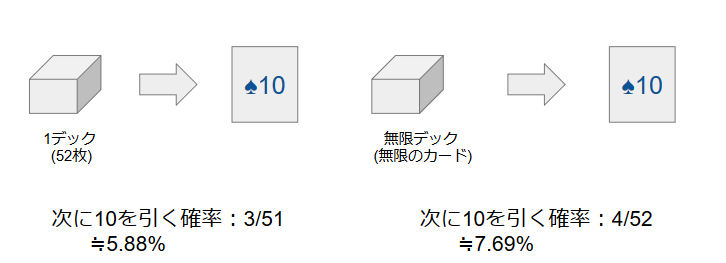
\includegraphics[width = 13cm]{./figure./DeckDiff.png}
%\caption{デック数による違い}
%\label{fig:deck}
%\end{center}
%\end{figure}

%\bunseki{※伊藤晋之介}

\section{戦略同士の比較}
Thorp(1962)によって提案されたベーシックストラテジーについて検証を行う。
ベーシックストラテジーの性能評価のために比較対象として6つの戦略を考えた。
比較対象となる戦略は次の通りである。

\begin{itemize}
  \item ベーシックストラテジー改変1
  \item ベーシックストラテジー改変2
  \item プレイヤーの合計値が15以上になるまでヒットする戦略
  \item プレイヤーの合計値が16以上になるまでヒットする戦略
  \item プレイヤーの合計値が17以上になるまでヒットする戦略
  \item プレイヤーの合計値が18以上になるまでヒットする戦略
\end{itemize}

以上の6つの戦略について、これから詳細に説明する。
\bunseki{※米村祥裕}

\subsection{ベーシックストラテジー改変1}
ベーシックストラテジーはブラックジャックにおける有効な戦略の一つである。しかし
戦略の表に注目すると、表の複雑性を考えたときに変更の余地があると考えた。
戦略表においてプレイヤーの合計値が12の行に注目する。ディーラーのアップカードが2、3の時は
Hとなっているが、その後アップカードが4、5、6の時はS、アップカードが7、8、9、10、Aの時はHとなっており、
Hに挟まれてSが存在している。表を覚えることを考えると、同じ行の中で変化が少ない方が複雑性が低いといえる。
そのため、ベーシックストラテジー改変1では表\ref{bschange1}に示すようにプレイヤーの合計値が12、ディーラーのアップカードが2、3の時の戦略をSに変更した。
\bunseki{※米村祥裕}

\begin{table}[htbp]
  \centering
  \caption{ベーシックストラテジー改変1\label{bschange1}}
  \begin{tabular}{|c|c|c|c|c|c|c|c|c|c|c|c|}
    \hline
    \multicolumn{2}{|c|}{} & \multicolumn{10}{|c|}{ディーラーのアップカード} \\ \hline
    \multicolumn{2}{|c|}{} & 2 & 3 & 4 & 5 & 6 & 7 & 8 & 9 & 10 & A \\ \hline
    手札の合計 & 19以上 & S & S & S & S & S & S & S & S & S & S \\ \cline{3-12}
              & 18 & S & S & S & S & S & S & S & S & S & S \\ \cline{3-12}
              & 17 & S & S & S & S & S & S & S & S & S & S \\ \cline{3-12}
              & 16 & S & S & S & S & S & H & H & H & H & H \\ \cline{3-12}
              & 15 & S & S & S & S & S & H & H & H & H & H \\ \cline{3-12}
              & 13~14 & S & S & S & S & S & H & H & H & H & H \\ \cline{3-12}
              & 12 & S & S & S & S & S & H & H & H & H & H \\ \cline{3-12}
              & 11以下 & H & H & H & H & H & H & H & H & H & H \\ \hline
  \end{tabular}
\end{table}

\subsection{ベーシックストラテジー改変2}
ベーシックストラテジー改変1と同様にベーシックストラテジーの戦略表を改変した。
変更点はベーシックストラテジー改変1と同様にプレイヤーの合計値が12の行である。改変1ではディーラーのアップカードが2、3の部分を
Sに変更したが、改変2では4、5、6をHに変更した。この変更によってプレイヤーの合計値が12の行はすべてHという表\ref{bschange2}ができた。
\bunseki{※米村祥裕}

\begin{table}[htbp]
  \centering
  \caption{ベーシックストラテジー改変2\label{bschange2}}
  \begin{tabular}{|c|c|c|c|c|c|c|c|c|c|c|c|}
    \hline
    \multicolumn{2}{|c|}{} & \multicolumn{10}{|c|}{ディーラーのアップカード} \\ \hline
    \multicolumn{2}{|c|}{} & 2 & 3 & 4 & 5 & 6 & 7 & 8 & 9 & 10 & A \\ \hline
    手札の合計 & 19以上 & S & S & S & S & S & S & S & S & S & S \\ \cline{3-12}
              & 18 & S & S & S & S & S & S & S & S & S & S \\ \cline{3-12}
              & 17 & S & S & S & S & S & S & S & S & S & S \\ \cline{3-12}
              & 16 & S & S & S & S & S & H & H & H & H & H \\ \cline{3-12}
              & 15 & S & S & S & S & S & H & H & H & H & H \\ \cline{3-12}
              & 13~14 & S & S & S & S & S & H & H & H & H & H \\ \cline{3-12}
              & 12 & H & H & H & H & H & H & H & H & H & H \\ \cline{3-12}
              & 11以下 & H & H & H & H & H & H & H & H & H & H \\ \hline
  \end{tabular}
\end{table}

\subsection{プレイヤーの合計値が一定以上になるまでヒットする戦略}
ディーラーがある程度有利な戦略を採用しているという仮定の下で、プレイヤーもディーラーと同じような行動を行う戦略を考えた。プレイヤーの手札の合計値が一定以上になるまでヒットするものとして、次の4つの戦略を用意した。
\begin{itemize}
  \item プレイヤーの合計値が15以上になるまでヒットする戦略
  \item プレイヤーの合計値が16以上になるまでヒットする戦略
  \item プレイヤーの合計値が17以上になるまでヒットする戦略
  \item プレイヤーの合計値が18以上になるまでヒットする戦略
\end{itemize}
\bunseki{※米村祥裕}

\begin{table}[H]
  \centering
  \caption{プレイヤーの合計値が15以上になるまでヒットする戦略\label{hitleq15}}
  \begin{tabular}{|c|c|c|c|c|c|c|c|c|c|c|c|}
    \hline
    \multicolumn{2}{|c|}{} & \multicolumn{10}{|c|}{ディーラーのアップカード} \\ \hline
    \multicolumn{2}{|c|}{} & 2 & 3 & 4 & 5 & 6 & 7 & 8 & 9 & 10 & A \\ \hline
    手札の合計 & 19以上 & S & S & S & S & S & S & S & S & S & S \\ \cline{3-12}
              & 18 & S & S & S & S & S & S & S & S & S & S \\ \cline{3-12}
              & 17 & S & S & S & S & S & S & S & S & S & S \\ \cline{3-12}
              & 16 & S & S & S & S & S & S & S & S & S & S \\ \cline{3-12}
              & 15 & S & S & S & S & S & S & S & S & S & S \\ \cline{3-12}
              & 13~14 & H & H & H & H & H & H & H & H & H & H \\ \cline{3-12}
              & 12 & H & H & H & H & H & H & H & H & H & H \\ \cline{3-12}
              & 11以下 & H & H & H & H & H & H & H & H & H & H \\ \hline
  \end{tabular}
\end{table}

\begin{table}[H]
  \centering
  \caption{プレイヤーの合計値が16以上になるまでヒットする戦略\label{hitleq16}}
  \begin{tabular}{|c|c|c|c|c|c|c|c|c|c|c|c|}
    \hline
    \multicolumn{2}{|c|}{} & \multicolumn{10}{|c|}{ディーラーのアップカード} \\ \hline
    \multicolumn{2}{|c|}{} & 2 & 3 & 4 & 5 & 6 & 7 & 8 & 9 & 10 & A \\ \hline
    手札の合計 & 19以上 & S & S & S & S & S & S & S & S & S & S \\ \cline{3-12}
              & 18 & S & S & S & S & S & S & S & S & S & S \\ \cline{3-12}
              & 17 & S & S & S & S & S & S & S & S & S & S \\ \cline{3-12}
              & 16 & S & S & S & S & S & S & S & S & S & S \\ \cline{3-12}
              & 15 & H & H & H & H & H & H & H & H & H & H \\ \cline{3-12}
              & 13~14 & H & H & H & H & H & H & H & H & H & H \\ \cline{3-12}
              & 12 & H & H & H & H & H & H & H & H & H & H \\ \cline{3-12}
              & 11以下 & H & H & H & H & H & H & H & H & H & H \\ \hline
  \end{tabular}
\end{table}

\begin{table}[H]
  \centering
  \caption{プレイヤーの合計値が17以上になるまでヒットする戦略\label{hitleq17}}
  \begin{tabular}{|c|c|c|c|c|c|c|c|c|c|c|c|}
    \hline
    \multicolumn{2}{|c|}{} & \multicolumn{10}{|c|}{ディーラーのアップカード} \\ \hline
    \multicolumn{2}{|c|}{} & 2 & 3 & 4 & 5 & 6 & 7 & 8 & 9 & 10 & A \\ \hline
    手札の合計 & 19以上 & S & S & S & S & S & S & S & S & S & S \\ \cline{3-12}
              & 18 & S & S & S & S & S & S & S & S & S & S \\ \cline{3-12}
              & 17 & S & S & S & S & S & S & S & S & S & S \\ \cline{3-12}
              & 16 & H & H & H & H & H & H & H & H & H & H \\ \cline{3-12}
              & 15 & H & H & H & H & H & H & H & H & H & H \\ \cline{3-12}
              & 13~14 & H & H & H & H & H & H & H & H & H & H \\ \cline{3-12}
              & 12 & H & H & H & H & H & H & H & H & H & H \\ \cline{3-12}
              & 11以下 & H & H & H & H & H & H & H & H & H & H \\ \hline
  \end{tabular}
\end{table}

\begin{table}[H]
  \centering
  \caption{プレイヤーの合計値が18以上になるまでヒットする戦略\label{hitleq18}}
  \begin{tabular}{|c|c|c|c|c|c|c|c|c|c|c|c|}
    \hline
    \multicolumn{2}{|c|}{} & \multicolumn{10}{|c|}{ディーラーのアップカード} \\ \hline
    \multicolumn{2}{|c|}{} & 2 & 3 & 4 & 5 & 6 & 7 & 8 & 9 & 10 & A \\ \hline
    手札の合計 & 19以上 & S & S & S & S & S & S & S & S & S & S \\ \cline{3-12}
              & 18 & S & S & S & S & S & S & S & S & S & S \\ \cline{3-12}
              & 17 & H & H & H & H & H & H & H & H & H & H \\ \cline{3-12}
              & 16 & H & H & H & H & H & H & H & H & H & H \\ \cline{3-12}
              & 15 & H & H & H & H & H & H & H & H & H & H \\ \cline{3-12}
              & 13~14 & H & H & H & H & H & H & H & H & H & H \\ \cline{3-12}
              & 12 & H & H & H & H & H & H & H & H & H & H \\ \cline{3-12}
              & 11以下 & H & H & H & H & H & H & H & H & H & H \\ \hline
  \end{tabular}
\end{table}

\subsection{複雑性の定義について}

プレイヤーに扱いやすい戦略とは何かについて戦略の複雑性を定義し、複雑性の低い戦略をプレイヤーに扱いやすい
戦略であるとした。戦略の複雑性はChaitin(1969)によって定義されたコルモゴロフ複雑性を参考に新たに定義した。
コルモゴロフ複雑性とは、ある文字列があったときに、その文字列を生成するためのプログラムの内、最小の命令長を
その文字列の複雑性であると定義したものである。

新たに定義した複雑性を算出するためには、まず戦略の表を文字列として文字列を圧縮する。
圧縮の方法としては、元の表を「連続する文字+連続して文字が出た回数」と変換することで文字列を圧縮した。
例として、「HHSSSHHHHH」という10文字からなる文字列を圧縮すると、「H2S3H5」となり、圧縮した後の文字列は6文字
となる。また「HHHHHHHHHH」という文字列を「H10」と圧縮したときのように、連続して同じ文字が出た回数が2桁の場合には
数字部分を1文字として数える。つまり「H10」の文字列長は2文字である。

圧縮した後の文字列長を元の表の大きさ(80)で割った数値を複雑性の定義とした。
\bunseki{※米村祥裕}

\subsection{各戦略の複雑性}

%用意した戦略は次のような8行の配列とし、それぞれの行に圧縮を行った。\\

%\begin{table}[H]
%\caption{ベーシックストラテジーの戦略表}
%\label{table:data_type}
%\begin{center}
%\begin{tabular}{|cc|c|c|c|c|c|c|c|c|c|c|}
%\hline
%                            &            & \multicolumn{10}{c|}{ディーラーのアップカード}     \\ \cline{3-12} 
%                            &            & 2 & 3 & 4 & 5 & 6 & 7 & 8 & 9 & 10 & A \\ \hline
%\multicolumn{1}{|l|}{手札の合計} & 19以上       & S & S & S & S & S & S & S & S & S  & S \\ \cline{2-12} 
%\multicolumn{1}{|l|}{}      & 18         & S & S & S & S & S & S & S & S & S  & S \\ \cline{2-12} 
%\multicolumn{1}{|l|}{}      & 17         & S & S & S & S & S & S & S & S & S  & S \\ \cline{2-12} 
%\multicolumn{1}{|l|}{}      & 16         & S & S & S & S & S & H & H & H & H  & H \\ \cline{2-12} 
%\multicolumn{1}{|l|}{}      & 15         & S & S & S & S & S & H & H & H & H  & H \\ \cline{2-12} 
%\multicolumn{1}{|l|}{}      & 13$\sim$14 & S & S & S & S & S & H & H & H & H  & H \\ \cline{2-12} 
%\multicolumn{1}{|l|}{}      & 12         & H & H & S & S & S & H & H & H & H  & H \\ \cline{2-12} 
%\multicolumn{1}{|l|}{}      & 11以下       & H & H & H & H & H & H & H & H & H  & H \\ \hline
%\end{tabular}
%\end{center}
%\end{table}

今回用意した戦略を、全て圧縮したのが表\ref{table:data_type}である。


%\begin{figure}[htbp]
%\begin{center}
%\includegraphics[width=15cm,bb=0 0 602 261]{2.png}
%\end{center}
%\caption{各戦略の圧縮した後の文字列と複雑性}
%\label{picture}
%\end{figure}

%\begin{table}[H]
%\caption{各戦略の圧縮した後の文字列と複雑性\label{table:data_type}}
%\begin{center}
%\begin{tabular}{|c|c|c|c|}
%\hline
%戦略           & 圧縮した後の文字列                                                                   & 文字列長 & 複雑性   \\ \hline
%ベーシックストラテジー         & \begin{tabular}[c]{@{}l@{}}S10S5H5S5H5S5H5S5H5S5H5H2S3H5H10\end{tabular} & 30   & 0.375 \\ \hline
%ベーシックストラテジー改変1      & S10S5H5S5H5S5H5S5H5S5H5S5H5H10                                              & 28   & 0.35  \\ \hline
%ベーシックストラテジー改変2      & S10S5H5S5H5S5H5S5H5S5H5H10H10                                               & 26   & 0.325 \\ \hline
%15以上になるまでヒットする戦略 & S10S10S10S10S10H10H10H10                                                    & 16   & 0.2   \\ \hline
%16以上になるまでヒットする戦略 & S10S10S10S10H10H10H10H10                                                    & 16   & 0.2   \\ \hline
%17以上になるまでヒットする戦略 & S10S10S10H10H10H10H10H10                                                    & 16   & 0.2   \\ \hline
%18以上になるまでヒットする戦略 & S10S10H10H10H10H10H10H10                                                    & 16   & 0.2   \\ \hline
%\end{tabular}
%\end{center}
%\end{table}

\begin{table}[H]
\caption{各戦略の圧縮した後の文字列と複雑性\label{table:data_type}}
\begin{center}
\begin{tabular}{|c|c|c|c|}
\hline
戦略           & 圧縮した後の文字列                                                                   & 文字列長 & 複雑性   \\ \hline
ベーシックストラテジー         & \begin{tabular}[c]{@{}l@{}}S10S10S10S5H5S5H5S5H5H2S3H5H10\end{tabular} & 26   & 0.325 \\ \hline
ベーシックストラテジー改変1      & S10S10S10S5H5S5H5S5H5S5H5H10                                              & 24   & 0.300  \\ \hline
ベーシックストラテジー改変2      & S10S10S10S5H5S5H5S5H5H10H10                                               & 22   & 0.275 \\ \hline
15以上になるまでヒットする戦略 & S10S10S10S10S10H10H10H10                                                    & 16   & 0.2   \\ \hline
16以上になるまでヒットする戦略 & S10S10S10S10H10H10H10H10                                                    & 16   & 0.2   \\ \hline
17以上になるまでヒットする戦略 & S10S10S10H10H10H10H10H10                                                    & 16   & 0.2   \\ \hline
18以上になるまでヒットする戦略 & S10S10H10H10H10H10H10H10                                                    & 16   & 0.2   \\ \hline
\end{tabular}
\end{center}
\end{table}

表\ref{table:data_type}を見ると、ベーシックストラテジーを改変した戦略の方が、複雑性が低く、プレイヤーにとって扱いやすいといえる。
また、手札の合計値が一定以上になるまでヒットする戦略は、複雑性がベーシックストラテジーの半分程度であり、プレイヤーに
とって扱いやすい戦略だといえる。
\bunseki{※渡邊凛}


\section{複雑性の検証実験}

\subsection{概要}

本プロジェクトの目標の要件を満たす戦略表を作成するには、人が扱いやすいということについて定量的に表し、既存、もしくは新たに作成した戦略表を評価しなければならない。そのため、前期ではコルモゴロフ複雑性を参考にし、連長圧縮を用いることで複雑性を定義し、これをある戦略表を記憶する難易度の評価指標として用いた。しかし、実際に人間がある戦略表を覚える時に感じる難易度と複雑性によって表した難易度は、異なっている可能性がある。そのため、後期では複雑性の検証実験として、いくつかの戦略表を用意し、記憶してもらうという実験を行うことで、複雑性が戦略表を記憶する難易度を正しく表しているかを確かめた。
\bunseki{※鳥谷航大}

\subsection{実験の目的}

本実験のもっとも重要な目的は、先述の通り、人が扱いやすい戦略表というのはどういう戦略表なのかを定量的に表すことである。そのため、本実験では、以下の2つを主な目的とした。
\begin{itemize}
    \item 目的1:本プロジェクトが定義した複雑性が戦略表を記憶する難易度を正しく表しているかを確認すること
    \item 目的2:目的1を達成出来なかった場合、可能な限り戦略表を記憶する難易度を正確に評価できる指標を見つけること
\end{itemize}
目的2について、具体的には、人のどのような能力がブラックジャックをプレイする能力と関連性を持つかや、個人の性格が実験に影響を及ぼすかなどの観点を中心に実験を行った。
\bunseki{※鳥谷航大}

\subsection{仮説}

私達は以下のような仮説を立て、実験を行った。
\begin{itemize}
    \item 仮説1:複雑性は人が戦略表を記憶する時に感じる難易度を正確に表すことが出来ない
    \item 仮説2:一般的な認知的判断能力と戦略表を扱う能力は同じ能力、もしくは深い関連性を持つ
    \item 仮説3:リスクを好む・好まない等の性格によって戦略表を記憶し扱う時に違いが生じる
\end{itemize}
それぞれの仮説に対して詳しく説明する。まず仮説1についてであるが、このような仮説を立てた背景として、前期でこの複雑性を用いて性能を評価した時、戦略表の勝率があまり良くない戦略表が高い性能と評価されてしまったことがある。このことから、他に戦略表を記憶する難易度を正確に表すことが出来る指標が存在するのではないか、と考えこのような仮説を立てた。そして、仮説2、仮説3は、先述の他の評価指標として考えられるものである。仮説2は、個人の一般的な認知判断能力が評価指標になるのではないかという仮説である。それに対して、仮説3は、個人のリスクに関する性格が評価指標になるのではないかという仮説である。
\bunseki{※鳥谷航大}

\subsection{実験準備}

今回の実験の目的や仮説に合わせ、実験に用いる戦略表や被験者、報酬などは以下のように準備を行った。
まず、今回の実験で用いた戦略表は以下の3つである。
% Please add the following required packages to your document preamble:

\begin{table}[H]
    \caption{戦略表A}
    \begin{center}
        \begin{tabular}{|c|c|c|c|c|c|c|c|c|c|c|c|}
        \hline
        \multicolumn{2}{|c|}{\multirow{2}{*}{}} & \multicolumn{10}{c|}{ディーラーのアップカード}     \\ \cline{3-12} 
        \multicolumn{2}{|c|}{}                  & 2 & 3 & 4 & 5 & 6 & 7 & 8 & 9 & 10 & A \\ \hline
        \multirow{10}{*}{手札の合計}      & 5〜8      & H & H & H & H & H & H & H & H & H  & H \\ \cline{2-12} 
                                    & 9        & H & H & H & H & H & H & H & H & H  & H \\ \cline{2-12} 
                                    & 10       & H & H & H & H & H & H & H & H & H  & H \\ \cline{2-12} 
                                    & 11       & H & H & H & H & H & H & H & H & H  & H \\ \cline{2-12} 
                                    & 12       & H & H & H & H & H & H & H & H & H  & H \\ \cline{2-12} 
                                    & 13       & H & H & H & H & H & H & H & H & H  & H \\ \cline{2-12} 
                                    & 14       & H & H & H & H & H & H & H & H & H  & H \\ \cline{2-12} 
                                    & 15       & H & H & H & H & H & H & H & H & H  & H \\ \cline{2-12} 
                                    & 16       & S & S & S & S & S & S & S & S & S  & S \\ \cline{2-12} 
                                    & 17以上     & S & S & S & S & S & S & S & S & S  & S \\ \hline
        \end{tabular}
    \end{center}
\end{table}

% Please add the following required packages to your document preamble:
% \usepackage{multirow}
\begin{table}[H]
    \begin{center}
    \caption{戦略表B}
    \begin{tabular}{|c|c|c|c|c|c|c|c|c|c|c|c|c|}
    \hline
    \multicolumn{3}{|c|}{\multirow{2}{*}{}}                     & \multicolumn{10}{c|}{ディーラーのアップカード}     \\ \cline{4-13} 
    \multicolumn{3}{|c|}{}                                      & 2 & 3 & 4 & 5 & 6 & 7 & 8 & 9 & 10 & A \\ \hline
    \multirow{28}{*}{手札の合計} & \multirow{9}{*}{ハードハンド}   & 9     & H & H & H & H & H & H & H & H & H  & H \\ \cline{3-13} 
                            &                           & 10    & H & D & D & D & D & H & H & H & H  & H \\ \cline{3-13} 
                            &                           & 11    & D & D & D & D & D & D & D & D & H  & H \\ \cline{3-13} 
                            &                           & 12    & D & D & D & D & D & D & D & D & D  & D \\ \cline{3-13} 
                            &                           & 13    & H & H & S & S & S & H & H & H & H  & H \\ \cline{3-13} 
                            &                           & 14    & S & S & S & S & S & H & H & H & H  & H \\ \cline{3-13} 
                            &                           & 15    & S & S & S & S & S & H & H & H & R  & H \\ \cline{3-13} 
                            &                           & 16    & S & S & S & S & S & H & H & R & R  & R \\ \cline{3-13} 
                            &                           & 17以上  & S & S & S & S & S & S & S & S & S  & S \\ \cline{2-13} 
                            & \multirow{9}{*}{ソフトハンド}   & A,2   & H & H & H & D & D & H & H & H & H  & H \\ \cline{3-13} 
                            &                           & A,3   & H & H & H & D & D & H & H & H & H  & H \\ \cline{3-13} 
                            &                           & A,4   & H & H & D & D & D & H & H & H & H  & H \\ \cline{3-13} 
                            &                           & A,5   & H & H & D & D & D & H & H & H & H  & H \\ \cline{3-13} 
                            &                           & A,6   & H & D & D & D & D & H & H & H & H  & H \\ \cline{3-13} 
                            &                           & A,7   & S & D & D & D & D & S & S & H & H  & H \\ \cline{3-13} 
                            &                           & A,8   & S & S & S & S & S & S & S & S & S  & S \\ \cline{3-13} 
                            &                           & A,9   & S & S & S & S & S & S & S & S & S  & S \\ \cline{3-13} 
                            &                           & A,10  & S & S & S & S & S & S & S & S & S  & S \\ \cline{2-13} 
                            & \multirow{10}{*}{スプリット可能} & A,A   & P & P & P & P & P & P & P & P & P  & P \\ \cline{3-13} 
                            &                           & 2,2   & P & P & P & P & P & P & H & H & H  & H \\ \cline{3-13} 
                            &                           & 3,3   & P & P & P & P & P & P & H & H & H  & H \\ \cline{3-13} 
                            &                           & 4,4   & H & H & H & P & P & H & H & H & H  & H \\ \cline{3-13} 
                            &                           & 5,5   & D & D & D & D & D & D & D & D & H  & H \\ \cline{3-13} 
                            &                           & 6,6   & P & P & P & P & P & H & H & H & H  & H \\ \cline{3-13} 
                            &                           & 7,7   & P & P & P & P & P & P & H & H & H  & H \\ \cline{3-13} 
                            &                           & 8,8   & P & P & P & P & P & P & P & P & P  & P \\ \cline{3-13} 
                            &                           & 9,9   & P & P & P & P & P & S & P & P & S  & S \\ \cline{3-13} 
                            &                           & 10,10 & S & S & S & S & S & S & S & S & S  & S \\ \hline
    \end{tabular}
    \end{center}
\end{table}

% Please add the following required packages to your document preamble:
% \usepackage{multirow}
\begin{table}[H]
    \begin{center}
    \caption{戦略表C}
    \begin{tabular}{|c|c|c|c|c|c|c|c|c|c|c|c|c|}
    \hline
    \multicolumn{3}{|c|}{\multirow{2}{*}{}}                     & \multicolumn{10}{c|}{ディーラーのアップカード}     \\ \cline{4-13} 
    \multicolumn{3}{|c|}{}                                      & 2 & 3 & 4 & 5 & 6 & 7 & 8 & 9 & 10 & A \\ \hline
    \multirow{28}{*}{手札の合計} & \multirow{9}{*}{ハードハンド}   & 9     & H & H & H & H & H & H & H & H & H  & H \\ \cline{3-13} 
                            &                           & 10    & H & D & D & D & D & H & H & H & H  & H \\ \cline{3-13} 
                            &                           & 11    & D & D & D & D & D & D & D & D & H  & H \\ \cline{3-13} 
                            &                           & 12    & D & D & D & D & D & D & D & D & D  & D \\ \cline{3-13} 
                            &                           & 13    & H & H & S & S & S & H & H & H & H  & H \\ \cline{3-13} 
                            &                           & 14    & S & S & S & S & S & H & H & H & H  & H \\ \cline{3-13} 
                            &                           & 15    & S & S & S & S & S & H & H & H & H  & H \\ \cline{3-13} 
                            &                           & 16    & S & S & S & S & S & H & H & H & H  & H \\ \cline{3-13} 
                            &                           & 17以上  & S & S & S & S & S & S & S & S & S  & S \\ \cline{2-13} 
                            & \multirow{9}{*}{ソフトハンド}   & A,2   & H & H & H & H & D & H & H & H & H  & H \\ \cline{3-13} 
                            &                           & A,3   & H & H & H & D & D & H & H & H & H  & H \\ \cline{3-13} 
                            &                           & A,4   & H & H & D & D & D & H & H & H & H  & H \\ \cline{3-13} 
                            &                           & A,5   & H & H & D & D & D & H & H & H & H  & H \\ \cline{3-13} 
                            &                           & A,6   & H & D & D & D & D & H & H & H & H  & H \\ \cline{3-13} 
                            &                           & A,7   & D & D & D & D & D & S & S & H & H  & H \\ \cline{3-13} 
                            &                           & A,8   & S & S & S & S & D & S & S & S & S  & S \\ \cline{3-13} 
                            &                           & A,9   & S & S & S & S & S & S & S & S & S  & S \\ \cline{3-13} 
                            &                           & A,10  & S & S & S & S & S & S & S & S & S  & S \\ \cline{2-13} 
                            & \multirow{10}{*}{スプリット可能} & A,A   & P & P & P & P & P & P & P & P & P  & P \\ \cline{3-13} 
                            &                           & 2,2   & H & H & P & P & P & P & H & H & H  & H \\ \cline{3-13} 
                            &                           & 3,3   & P & P & P & P & P & P & H & H & H  & H \\ \cline{3-13} 
                            &                           & 4,4   & H & H & H & P & P & H & H & H & H  & H \\ \cline{3-13} 
                            &                           & 5,5   & D & D & D & D & D & D & D & D & H  & H \\ \cline{3-13} 
                            &                           & 6,6   & P & P & P & P & P & H & H & H & H  & H \\ \cline{3-13} 
                            &                           & 7,7   & P & P & P & P & P & P & H & H & H  & H \\ \cline{3-13} 
                            &                           & 8,8   & P & P & P & P & P & P & P & P & P  & P \\ \cline{3-13} 
                            &                           & 9,9   & P & P & P & P & P & S & P & P & S  & S \\ \cline{3-13} 
                            &                           & 10,10 & S & S & S & S & S & S & S & S & S  & S \\ \hline
    \end{tabular}
    \end{center}
\end{table}
またこれらの戦略表の複雑性は以下の表のとおりである。
\begin{table}[H]
    \begin{center}
    \caption{各戦略表の複雑性}
    \begin{tabular}{|c|c|c|c|}
        \hline
            & 戦略表A & 戦略表B  & 戦略表B  \\ \hline
        複雑性 & 0.2  & 0.448 & 0.407 \\ \hline
    \end{tabular}   
    \end{center}
\end{table}

次に被験者についてである。被験者は本学の学生から募集をした。募集方法としては、ブラックジャックに関する実験であることや、戦略表を記憶するテストであるなどの実験の内容を事前に知らせずに募集した。募集の結果、男性15人、女性5人の計20人集めることが出来た。被験者の年齢は18〜21歳であった。

今回20人の被験者が集まったため実験時に2つのグループに分けて実験を行った。分けられたグループは記憶する戦略表が異なる。具体的な分け方は以下のとおりである。
\begin{itemize}
    \item グループX:戦略表A、Bを記憶するグループ
    \item グループY:戦略表A、Cを記憶するグループ
\end{itemize}
このようにグループ分けした理由としては、比較的複雑性の低い戦略表Aの成績を確認することで、戦略表Bと戦略表Cの成績の違いの要因が、戦略表の複雑性によってなのか個人差によってなのかを確認するためである。

最後に実験協力の報酬についてである。報酬は実験前に、実験結果の成績に応じて配られるという説明を行い、成績が高い被験者ほど多くの報酬が得られるように分配した。
\bunseki{※鳥谷航大}

\subsection{実験の手法・手順}

今回の実験は、異なる複雑性を持つ戦略表を3つ用意し、先述したグループごとに対応する戦略表を記憶してもらった後テストを行うというものである。その後、CRT(Cognitive Reflection Test)やリスク回避性のテストなどを行い、テストの成績との関連性を分析した。詳しい実験手順は以下のとおりである。
\begin{enumerate}
    \item ブラックジャックについての説明を行う
    \item 5〜10分程度の時間を用いて実際にプレイしゲームを理解してもらう
    \item 戦略表を配り10分間で記憶してもらう
    \item テストを配り7分間で回答してもらう
    \item 回答を配り被験者に採点をしてもらいテストを回収する
    \item 4〜6を戦略表を変更しもう一度繰り返す
    \item CRTとリスク回避性のテストについて回答してもらう。回答時間は両方合わせて10〜15分とした。
    \item 結果に応じた報酬を配り実験を終了する
\end{enumerate}
\bunseki{※鳥谷航大}

\subsection{実験結果}

今回の実験で得られた主な結果は以下の3つである。
\begin{itemize}
    \item 結果1:テストの成績と複雑性には強い負の相関があること
    \item 結果2:CRTの点数とテストの成績には相関がないこと
    \item 結果3:リスク回避性とテストの成績には相関がないこと
\end{itemize}
ここでは、私達が特に興味深く感じた結果1,2に関して詳しく説明していく。

以下はそれぞれのグループの成績である。また、戦略表のテストは満点が30点であり、CRTの満点は11点である。
\begin{table}[H]
    \begin{center}
    \caption{グループXの成績}
    \begin{tabular}{|c|c|c|c|}
    \hline
         & 戦略表A & 戦略表B  & CRT   \\ \hline
    平均   & 29.1 & 13.8  & 7.2   \\ \hline
    分散   & 2.29 & 12.96 & 3.96  \\ \hline
    標準偏差 & 1.51 & 3.6   & 2.098 \\ \hline
    \end{tabular}
    \end{center}
\end{table}

\begin{table}[H]
    \begin{center}
    \caption{グループYの成績}
    \begin{tabular}{|c|c|c|c|}
    \hline
         & 戦略表A & 戦略表C  & CRT   \\ \hline
    平均   & 29.8 & 17.5  & 8.8   \\ \hline
    分散   & 0.6  & 2.872 & 1.36  \\ \hline
    標準偏差 & 0.36 & 8.25  & 1.229 \\ \hline
    \end{tabular}
    \end{center}
\end{table}
両方のグループともに、戦略表Aは高い成績となった。そのため、成績とCRT正答率つまり、一般的な認知的判断能力の相関関係を見る時には、戦略表Aから戦略表BまたはCの点数を引いた差とCRT正答率との相関を考えた。以下がその散布図である。
\begin{figure}[H]   
    \begin{center}
        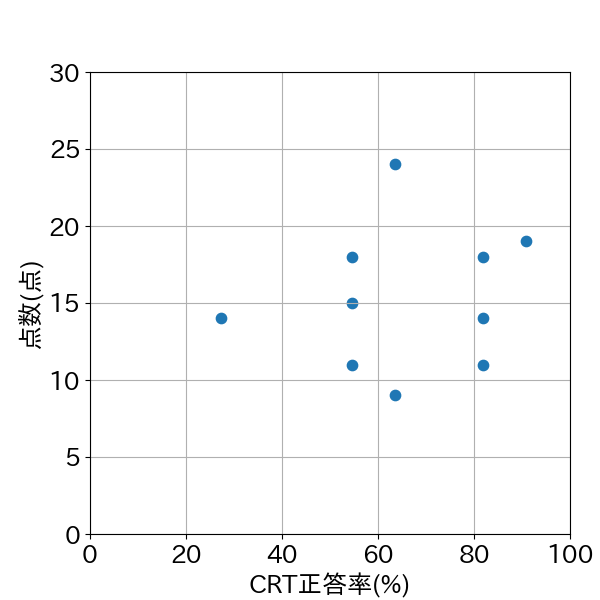
\includegraphics[width=10cm]{figure/groupX_crt_diffAB.png}
        \caption{CRT正答率と戦略表Aから戦略表Bの点数を引いた値との散布図}
    \end{center}
\end{figure}

\begin{figure}[H]
    \begin{center}
        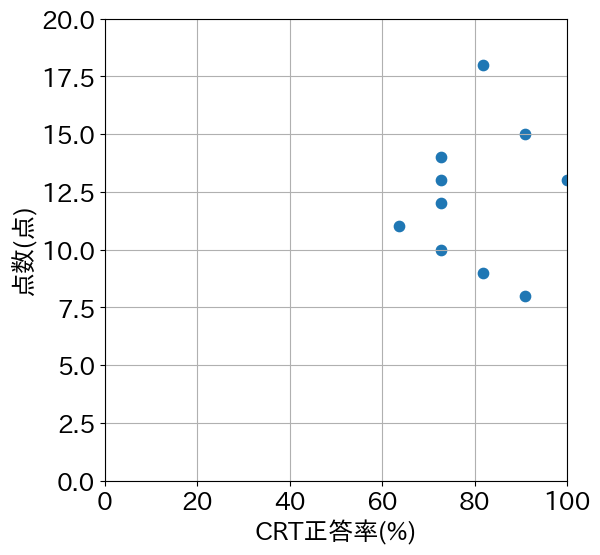
\includegraphics[width=10cm]{figure/groupY_crt_diffAC.png}
        \caption{CRT正答率と戦略表Aから戦略表Cの点数を引いた値との散布図}
    \end{center}
\end{figure}
また、この散布図より相関係数を求めたところ以下のようになった。
\begin{table}[H]
    \begin{center}
    \caption{それぞれのグループの相関係数}
    \begin{tabular}{|c|c|c|}
    \hline
                  & グループX & グループY \\ \hline
    CRTと点数の差の相関係数 & 0.145 & 0.079 \\ \hline
    \end{tabular}
    \end{center}
\end{table}
上の表の通り、相関係数は非常に小さいという結果になった。ただし、相関係数が小さくても相関がある可能性があるため、無相関検定を行った。無相関検定の検定条件などは後述の複雑性と成績の相関係数と合わせて詳しく後で述べる。無相関検定の結果、グループX、グループYともに相関が無いことがわかった。

次に、複雑性とテストの成績の関連性についてである。以下の表が各戦略表の複雑性とテストの平均点である。
\begin{table}[H]
    \begin{center}
        \caption{各戦略表の複雑性とテストの平均点}
    \begin{tabular}{|c|c|c|c|c|}
    \hline
            & 戦略表A(グループX) & 戦略表A(グループY) & 戦略表B  & 戦略表C  \\ \hline
    テストの平均点 & 29.1        & 29.8        & 13.8  & 17.5  \\ \hline
    複雑性     & 0.2         & 0.2         & 0.448 & 0.407 \\ \hline
    \end{tabular}
    \end{center}
\end{table}
さらに、実験で得られたデータを用いて成績と複雑性の相関係数を求めたところ$-0.942$となり、ほぼ$-1$に近い値となった。こちらも無相関検定を行ったところ、非常に強い負の相関があるという結果になった。
\bunseki{※鳥谷航大}

\subsection{実験結果の検定と分析}

ここでは、先程の無相関検定についての説明と各戦略表のテストの平均点に差があるかどうかを調べるために行った分散分析と多重比較について述べる。

まずは無相関検定についてである。以下がグループX・グループYの成績とそれぞれのCRTの正答率との相関を調べる無相関検定の検定条件の表である。
\begin{table}[H]
    \begin{center}
        \caption{無相関検定の検定条件}        
        \begin{tabular}{|c|c|c|}
        \hline
            & グループX          & グループY          \\ \hline
        帰無仮説 & \multicolumn{2}{c|}{相関係数が0}     \\ \hline
        対立仮説 & \multicolumn{2}{c|}{相関係数が0ではない} \\ \hline
        相関係数 & 0.145          & 0.079          \\ \hline
        自由度  & \multicolumn{2}{c|}{8}          \\ \hline
        T値   & 0.415          & 0.224          \\ \hline
        有意水準 & \multicolumn{2}{c|}{0.05}       \\ \hline
        P値   & 0.689          & 0.829          \\ \hline
        \end{tabular}
    \end{center}
\end{table}
以上より、先述の通り、グループX・グループYともに相関係数は0となり、CRTの正答率とテストの成績には相関がないことが確認された。

次に、複雑性とテストの成績に関する無相関検定である。同様に、以下が検定条件の表である。
\begin{table}[H]
    \begin{center}
        \caption{無相関検定の検定条件}
        \begin{tabular}{|c|c|}
        \hline
            & 複雑性と成績     \\ \hline
        帰無仮説 & 相関係数が0     \\ \hline
        対立仮説 & 相関係数が0ではない \\ \hline
        相関係数 & -0.942     \\ \hline
        自由度  & 18         \\ \hline
        T値   & 7.963      \\ \hline
        有意水準 & 0.05       \\ \hline
        P値   & 0.000      \\ \hline
        \end{tabular}
    \end{center}
\end{table}
以上より、こちらも先述の通り、複雑性とテストの成績には強い負の相関があることが確認された。

次に、多重比較と分散分析についてである。今回の実験では、戦略表Aの複雑性が0.2となっていたためか、他のテストの成績に比べとても高い成績となった。そのため、先述の相関係数が負の相関を表したことが戦略表Aの結果に強く影響を受けている可能性や、B,C間の成績に違いがない可能性があるため分散分析と多重比較を行った。以下が、その検定条件と結果である。
\begin{table}[H]
    \begin{center}
        \caption{分散分析と多重比較の検定条件}
        \begin{tabular}{|c|c|c|c|c|}
        \hline
            & 全ての戦略表間       & A-B間     & A-C間     & B-C間     \\ \hline
        帰無仮説 & 各戦略表の平均点に差がない & \multicolumn{3}{c|}{戦略表間に差がない} \\ \hline
        対立仮説 & 各戦略間に差がある     & \multicolumn{3}{c|}{戦略間に差がある}  \\ \hline
        有意水準 & \multicolumn{4}{c|}{0.05}                      \\ \hline
        P値   & 0.000         & 0.000    & 0.000    & 0.007    \\ \hline
        \end{tabular}
    \end{center}
\end{table}
以上より、全ての戦略表の成績に差があり、かつ全ての戦略表間の成績に差があるという結果になった。
\bunseki{※鳥谷航大}

\subsection{考察}

以上の結果を全てまとめると、以下のようになる。
\begin{itemize}
    \item 結果1:複雑性とテストの成績には強い負の相関がある
    \item 結果2:CRTの正答率とテストの成績には相関がない
    \item 結果3:リスク回避性とテストの成績には相関がない
\end{itemize}
以上の実験結果より、以下のようにまとめることが出来る。
\begin{itemize}
    \item 考察1:戦略表の複雑性が高いほどテストの成績は悪くなるため、複雑性は評価指標として適している
    \item 考察2:ブラックジャックの戦略を用いる能力は一般的な認知的判断能力とは異なる
    \item 考察3:個人のリスクを好むかどうかなどの正確はブラックジャックをプレイする上で大きな影響は与えない
\end{itemize}
以上より、本プロジェクトで定義した複雑性が適していることが確認されたため、実験は概ね成功だった。しかし、ブラックジャックをプレイするのに必要な能力が明確になっていないため、今後の実験で検証していきたい。
\bunseki{※鳥谷航大}

\chapter{遺伝的アルゴリズム}
\section{遺伝的アルゴリズム}
\subsection{概要}
本研究の目的は、ブラックジャックにおいてプレイヤーの利得を増加させ、かつ定義した
複雑性がより小さくなるような戦略を発見することである.そのために我々はプレイヤーの
勝率、戦略の複雑性の数値から性能1、性能2という2つの評価値を設定した。
戦略はプレイヤーの手札、ディーラーのアップカードを軸とする表で表される。評価値を
大きくするような戦略を見つけることは、一般的には最適化問題と分類される。
本研究で扱っているブラックジャックというゲームは、既に使用されたカードによって
後のプレイにおける、カードの出現確率が変動する。そのため単純な式でゲームの進行を表現するのは
現在のところ困難であり,プレイヤーの行動とゲームの結果のみを用いて戦略の最適化を
行う必要がある。

また、ブラックジャックの戦略は18行10列の表で表すことができる。単純にヒット、スタンドを行うという制限を
付けた場合でも、2の180乗通りの戦略表が考えられる。この通り数は膨大であり、単純に全探索を行うには非現実的な
時間を要する。

そのため本研究では入出力の関係から最適なパラメータを探索するアルゴリズムのなかで,生物の進化過程を模した、遺伝的アルゴリズム
という手法によって最適な戦略を発見することを試みた.遺伝的アルゴリズムは数ある探索対象の中から効率的に解を探索するため、
膨大な探索範囲を持つ戦略表に対して適していると考え使用した。
\bunseki{※米村祥裕}

\subsection{アルゴリズムの説明}
遺伝的アルゴリズムは生物の遺伝メカニズムをアイデアの中心として考案された最適化アルゴリズムの一つである。遺伝的アルゴリズムは次の工程からなる。
  \begin {enumerate}
    \item 初期個体群の生成
    \item 各個体の環境への適応度の評価
    \item 選択アルゴリズムによって次世代個体の親となる個体を抽出
    \item 交叉アルゴリズムによって親個体から次世代個体を生成
    \item 次世代個体に対して突然変異を適用
    \item 2から4を、次世代個体が必要数に達するまで繰り返し実行
    \item 2から5を、適応度が一定以上になるか最大世代になるまで繰り返し実行
  \end {enumerate}

本プロジェクトにおいて、個体とは戦略表に相当し、環境への適応度は、ブラックジャックをプレイした時の性能に相当する。

これから、遺伝的アルゴリズムにおいて個体がどのように表現されるのかについて遺伝子コーディングという項目で説明する。
また遺伝子コーディングの説明を使って、選択アルゴリズム、交叉アルゴリズム、突然変異について説明する。

\bunseki{※米村祥裕}

\subsection{遺伝子コーディング}
遺伝子コーディングとは探索対象となっている問題を遺伝子配列として扱うために対応させる作業である。生物の遺伝子には遺伝子型(genotype)と表現型(phenotype)とがある。
遺伝子型とは遺伝子の配列のことで、表現型とは遺伝子型によって現れる形質のことである。そのため遺伝子型として存在していても発現しない形質も当然存在する。遺伝子コーディングにおいては
探索対象においての一つの解パターンが表現型、解パターンを表現するための情報配列が遺伝子型に対応する。情報配列としては単純に0と1のいずれかの数値を要素としてもつバイナリ配列や
順序関係を番号で表した順序配列、または文字配列などがある。巡回セールスマン問題で遺伝的アルゴリズムを適用する場合には順序配列に巡回順序をそのまま記述するなど、情報配列がそのまま表現型になる場合もある。

本プロジェクトにおいて、遺伝的アルゴリズムを使用したシミュレーションでは、ヒットとスタンドからなる戦略についてのみ探索を行ったため、バイナリ配列を用い、表現型として現れる
戦略は、配列上の対応する位置の要素が0であればヒット、1であればスタンドであるという変換によって遺伝子コーディングを実装した。
\bunseki{※米村祥裕}

\subsection{選択アルゴリズム}
\subsubsection{ルーレット選択方式}
ルーレット選択方式とは、各個体が選ばれる確率を、適応度に比例する式で決定するアルゴリズムである。そのため適応度比例選択方式とも呼ばれる。
ルーレット選択方式において、各個体$i$の適応度を$f_i$として、個体$i$が親個体として選択される確率$P(i)$は次の式で定義される。
$$P(i) = \frac{f_i}{\sum_k f_k}$$
\subsubsection{エリート保存方式}
エリート保存方式とは現世代における、最大の適応度である個体を次世代個体に登録する方式である。ルーレット選択では、親個体の選択が確率的に行われることから、
次世代個体が現世代個体の性能を下回ることが十分に考えられる。そこで、最大の性能の個体を次世代でも作ることで性能の低下を防ぐことができる。
\bunseki{※米村祥裕}

\subsection{交叉アルゴリズム}
\subsubsection{一様交叉アルゴリズム}
一様交叉アルゴリズムでは、まず個体の遺伝子長と同じ大きさのバイナリ配列を生成する。この時バイナリ配列上には0と1が並ぶが、各要素が0と1のいずれに
なるかはランダムに決定する。こうしてできたバイナリ配列をビットマスクという。2つの親個体の対応する遺伝子を$K_1, K_2$として,それらの遺伝子に対応する
ビットマスク上の要素を$M$と表記する。$M$の値に応じて次のように交叉を適用し、次世代個体$k_1, k_2$を生成する。
  \begin{itemize}
    \item $M = 0$なら$k_1 \leftarrow K_2, k_2 \leftarrow \overline{K_1}$
    \item $M = 1$なら$k_1 \leftarrow K_1, k_2 \leftarrow K_1$
  \end{itemize}
遺伝子長と同じ長さのマスクを生成し、対応するマスクの値によって交叉を変化させるものであれば一様交叉と言われるため、上記のものとは異なる実装も考案されている。
\bunseki{※米村祥裕}

\subsection{突然変異アルゴリズム}
個体に変化が起きなくなると、新しい解を探索することができなくなるため、それを防ぐために個体の遺伝子情報をランダムに変化させるのが
突然変異アルゴリズムである。突然変異アルゴリズムでは、生成されたすべての次世代個体のすべての遺伝子配列上要素について、あらかじめ設定した
確率で次の変更を行う。
  \begin{itemize}
    \item 元の要素が0なら1にする
    \item 元の要素が1なら0にする
  \end{itemize}
\bunseki{※米村祥裕}

\subsection{実験条件}
遺伝的操作についてのパラメータは表に示すように設定した。

  \begin{table}[htb]
    \centering
    \label{geneticparameter}
    \caption{遺伝的操作のパラメータ}
    \begin{tabular}{|c|c|} \hline
      遺伝子長 & 180 \\ \hline
      個体数 & 200 \\ \hline
      適応度 & 勝率 $\div$ 複雑性 \\ \hline
      最大世代数 & 10000 \\ \hline
      交叉率 & 0.85 \\ \hline
      突然変異率 & 0.006 \\ \hline
    \end{tabular}
  \end{table}

個体数の設定については様々な方針が提案されているが、今回は遺伝子長よりも多い数の個体を用意するというものにした。
突然変異率については遺伝子長の逆数とするという方法が考案されていたため、採用した。今回の場合だと$1/180$となっている。

また、初期個体として、ベーシックストラテジーを行う個体を5個体、14以上でスタンドする個体を5個体、15以上でスタンドする個体を5個体、16以上でスタンドする個体を5個体それぞれ設定した。
これは、事前の実験で完全にランダムな初期個体のみだと上手く性能が向上しないということが明らかであったからである。

ブラックジャックのゲームを行うときの条件は次のように設定した。

\begin{itemize}
\item デック数は無限
\item ゲーム数は5万回
\end{itemize}

ベーシックストラテジーと比較するため、前提条件として無限デックである設定にしてゲームを行わせた。
\bunseki{※米村祥裕}

\subsection{実験結果}
遺伝的アルゴリズムによるシミュレーションを行った結果、図\ref{gaprocess}に示すような性能の推移となった。図\ref{gaprocess}中のmaxは最優秀性能の個体の適応度を
表している。minは最低性能の個体の適応度、meanは全個体の適応度の平均値、medianは全個体の適応度の中央値、top\_meanは上位10個体の適応度の平均値、
top\_medianは上位10個体の適応度の中央値を表している。

全個体の平均適応度、及び中央値はおおよそ同じように推移している。初期個体群に比べるとGAの進行によって適応度は上昇している。しかし、全体の世代で通して見ると
振動しているもののほぼ横ばいになっている。同様に上位10個体の適応度の平値、中央値も振動しているが横ばいになっている。また、上位10個体の適応度は初期個体群の場合と
比べて大きく低下しているが、これは初期個体として与えた優秀な戦略が遺伝的操作による変更で変化したことによるものである。
個体の適応度の停滞が起こっていることが全体として推察されるが、最優秀個体の適応度は順調な上昇をしているため、遺伝的操作自体は
ある程度成功していると考えられる。

  \begin{figure}[htbp]
    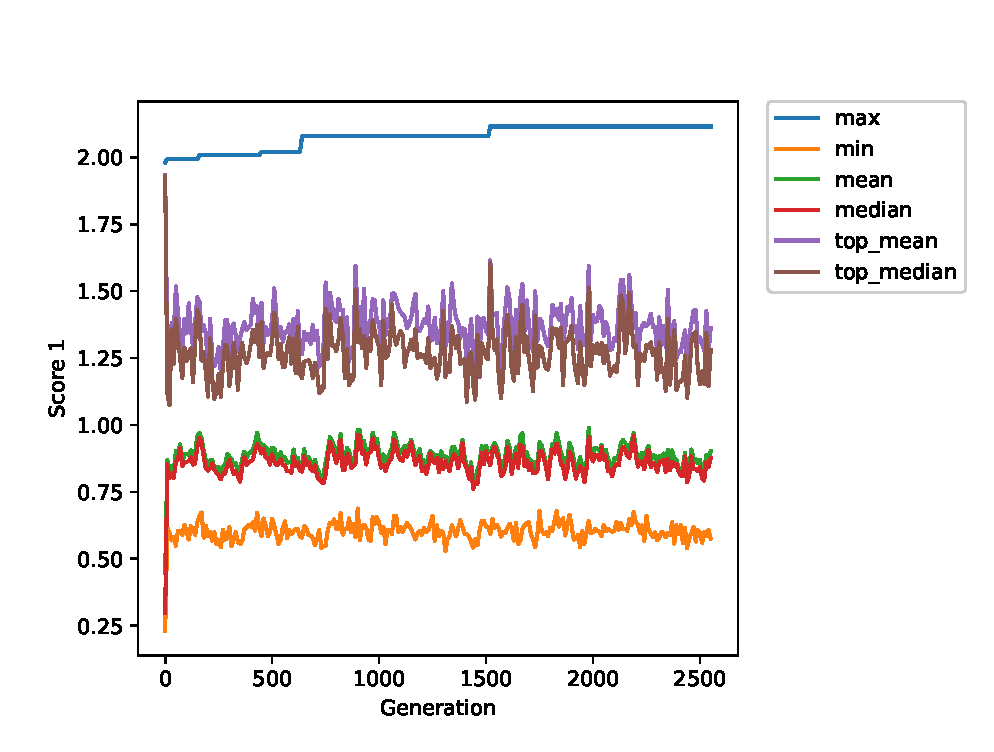
\includegraphics[width=14.0cm]{figure/gaprocess.eps}
    \caption{遺伝的アルゴリズムによるシミュレーションの進行}
    \label{gaprocess}
  \end{figure}

結果として得られた最優秀な個体の戦略が表\ref{gastrategyhard}、表\ref{gastrategysoft}である。
ハードハンドでは、13以下はすべてヒット、14以上でスタンドという戦略になっている。
ソフトハンドでは、ヒットとスタンドのみのベーシックストラテジーに対してプレイヤーの手札がA7でディーラーのアップカードが
9の時がヒットからスタンドに変わっており、プレイヤーの手札がA7でディーラーのアップカードがAの時がスタンドからヒットに変わっているという形になっている。

  \begin{table}[htbp]
    \centering
    \caption{GA戦略(ハードハンド)\label{gastrategyhard}}
    \begin{tabular}{|c|c|c|c|c|c|c|c|c|c|c|c|}
      \hline
      \multicolumn{2}{|c|}{} & \multicolumn{10}{|c|}{ディーラーのアップカード} \\ \hline
      \multicolumn{2}{|c|}{} & 2 & 3 & 4 & 5 & 6 & 7 & 8 & 9 & 10 & A \\ \hline
      手札の合計 & 19以上 & S & S & S & S & S & S & S & S & S & S \\ \cline{3-12}
                & 18 & S & S & S & S & S & S & S & S & S & S \\ \cline{3-12}
                & 17 & S & S & S & S & S & S & S & S & S & S \\ \cline{3-12}
                & 16 & S & S & S & S & S & S & S & S & S & S \\ \cline{3-12}
                & 15 & S & S & S & S & S & S & S & S & S & S \\ \cline{3-12}
                & 14 & S & S & S & S & S & S & S & S & S & S \\ \cline{3-12}
                & 13 & H & H & H & H & H & H & H & H & H & H \\ \cline{3-12}
                & 12 & H & H & H & H & H & H & H & H & H & H \\ \cline{3-12}
                & 11以下 & H & H & H & H & H & H & H & H & H & H \\ \hline
    \end{tabular}
  \end{table}

  \begin{table}[htbp]
    \centering
    \caption{GA戦略(ソフトハンド)\label{gastrategysoft}}
    \begin{tabular}{|c|c|c|c|c|c|c|c|c|c|c|c|}
      \hline
      \multicolumn{2}{|c|}{} & \multicolumn{10}{|c|}{ディーラーのアップカード} \\ \hline
      \multicolumn{2}{|c|}{} & 2 & 3 & 4 & 5 & 6 & 7 & 8 & 9 & 10 & A \\ \hline
      手札の合計 & AA & H & H & H & H & H & H & H & H & H & H \\ \cline{3-12}
                & A2 & H & H & H & H & H & H & H & H & H & H \\ \cline{3-12}
                & A3 & H & H & H & H & H & H & H & H & H & H \\ \cline{3-12}
                & A4 & H & H & H & H & H & H & H & H & H & H \\ \cline{3-12}
                & A5 & H & H & H & H & H & H & H & H & H & H \\ \cline{3-12}
                & A6 & H & H & H & H & H & H & H & H & H & H \\ \cline{3-12}
                & A7 & S & S & S & S & S & S & S & S & H & H \\ \cline{3-12}
                & A8 & S & S & S & S & S & S & S & S & S & S \\ \cline{3-12}
                & A9 & S & S & S & S & S & S & S & S & S & S \\ \hline
    \end{tabular}
  \end{table}

\bunseki{※米村祥裕}

\section{まとめ・手法の問題点}
\section{まとめ・手法の問題点
}
\subsection{SGAの概要と問題点}
この項では遺伝的アルゴリズムの問題点について説明していく。佐藤ら(1997)は代表的な遺伝的アルゴリズムでの世代交代モデルとしてSimple GA(以下SGAと表記する)を挙げ、そのモデルの問題点と改善案を示している。ただし、ここでは適応度をもとにした選択処理についての問題点と改善案を挙げており、交叉アルゴリズムや遺伝子のコード設計、各種パラメータの設定に関しては扱っていない。

世代交代のモデルには、次世代の個体を生成するための親を選択する複製選択と、全ての個体の中から次世代に残す個体を選択する生存選択の2種類の処理が存在する。SGAの場合この2つの選択処理は次のようになっている。

\begin{itemize}
\item{複製選択}\\
適応度に比例した選択確率を用いたルーレット選択方式によって、集団から個体を復元抽出する。
復元抽出とは一度選択された個体も次以降の選択対象に含める、つまり同じ個体が複数回選ばれることを許している選択方法である。
\item{生存選択}\\
無条件で親集団と生成された子集団のすべてを入れ替える。
\end{itemize}

佐藤ら(1997)によるとSGAには3つの問題点があることが指摘されている。
\begin{enumerate}
\item{高い選択圧下での早期収束}
\begin{itemize}
\item{SGAのように適応度を用いてルーレット選択を行っている場合、探索の初期に適応度が突出した個体が存在するとその個体が複製選択において選ばれる可能性が高くなりすぎてしまう。そうなった場合、探索の序盤からその個体に遺伝子全体が収束してしまう現象が起きてしまい、最適な解にたどりつきづらくなってしまう。この現象は初期収束と呼ばれている。}
\end{itemize}
\item{低い選択圧下での停滞}
\begin{itemize}
\item{遺伝的アルゴリズムの探索が進み、各世代の個体間の適応度に差が見られなくなってきた時に複製選択においてルーレット選択の効果が弱くなることがある。そうなると個体が最適な解に向かって進みづらくなってしまう現象が起こることがある。ここでは進化的停滞と呼んでいる。}
\end{itemize}
\item{優秀な遺伝子の破壊}
\begin{itemize}
\item{SGAでは親から子に世代が移る時は無条件で全ての遺伝子を入れ替えてしまう。そのため親個体に適応度の高い個体が存在する場合でもその個体は次の世代では失われてしまう。そのため集団から適応度の高い個体が失われてしまう可能性がある。}
\end{itemize}
\end{enumerate}
\bunseki{伊藤晋之介}

\subsection{SGAの改善案の紹介}
前項で挙げられたようにSGAの世代交代モデルには、初期収束、進化的停滞などの様々な問題点が存在している。これらの問題点を解決するため、佐藤ら(1997)ではSGAの複製選択アルゴリズムと、生存選択アルゴリズムを変更したいくつかの世代交代モデルが紹介されている。

\subsubsection{Iterated Genetic Search(IGS)}
\begin{itemize}
\item{複製選択}\\
適応度を無視して集団から個体をランダムに非復元抽出する。非復元抽出とは、同じ個体を1度しか選択しない選び方のこと。
\item{生存選択}\\
適応度の平均以下の個体をランダムに選び、生成された子個体のうち数体と入れ替える。
\end{itemize}
このモデルでは親個体の選択に適応度を用いず、ランダムに選択している。そのため上で挙げられた初期収束に陥る可能性を避けることができる。生存選択の時には適応度が平均以下の個体を子世代に混ぜることで、適応度が高い個体同士からは作り出せない新たな個体が生成されることを期待できる。そのため効率的に探索を行える可能性がある。

\subsubsection{Steady State(SS)}
\begin{itemize}
\item{複製選択}\\
ランキング選択法を用いて集団から個体を復元抽出する。
\item{生存選択}\\
親集団から最悪個体を選び、生成された子個体と入れ替える。
\end{itemize}
このモデルでは複製選択にランキング選択法を用いている。ランキング選択法とは親個体を選ぶ際に適応度が高い順に個体に順位をつけていく。そして順位に応じてその個体が選択される数を決める方法。ルーレット選択方式に比べ、極端に適応度が高い個体が存在する場合でもその個体以外の個体も確実に選ばれることを保証できる。そのため初期収束してしまう可能性を抑えることができる。生存選択ではIGSと同じように適応度の低い個体をいくつか混ぜることで、新たな個体が生成されることを期待できる。

\subsubsection{CHC}
\begin{itemize}
\item{複製選択}\\
適応度を無視して集団から個体をランダムに非復元抽出する。
\item{生存選択}\\
親集団と子集団を合わせた2世代の中から、適応度の高い順に集団サイズ分の個体を次世代に残す。
\end{itemize}
複製選択については個体をランダムに選択し初期収束を回避している。生存選択では親個体をすべて子個体と入れ替えるのではなく、親世代と子世代を合わせたものの中から適応度順に集団サイズ分だけ選んでいる。この処理を行うことで、親世代の個体が次世代以降も生き残る可能性が出てくる。そうすることで親個体に存在した優秀な個体が世代交代で失われるのを防ぐことができる。

\subsubsection{Elitist Recombination(ER)}
\begin{itemize}
\item{複製選択}\\
適応度を無視して集団から個体をランダムに非復元抽出する。
\item{生存選択}\\
各家族、すなわち親として選ばれた2個体とそこから生成された子の2個体の中から適応度の高い2個体を次世代に残す。
\end{itemize}
複製選択では初期収束を回避するため個体をランダムに選択している。生存選択では各家族間で適応度を比べ優秀なものが生き残るようになっている。そのため親世代の優秀な個体が失われることを防ぐことができる。またCHCとは異なり適応度の比較が家族間で行われることで、優秀な個体が急激に集団に広まることを防ぐ効果もある。
\bunseki{伊藤晋之介}

\subsection{今回設計したGAのまとめと改善案}
\subsubsection{まとめ}
今回我々が作成した遺伝的アルゴリズムでは、親世代で最も優秀な個体を次世代に残すエリート保存方式を採用している。そのため上記の問題点で挙げている優秀な遺伝子の破壊が起きる可能性は低いと考えられる。図\ref{gaprocess}からもわかる通り最優秀個体の適応度は減少してはいない。\\
問題点としては、初期個体にブラックジャックの基本戦略、14以上でスタンドする戦略、15以上でスタンドする戦略、16以上でスタンドする戦略をそれぞれ5個体ずつ設定したことが挙げられる。今回は遺伝的アルゴリズムの実行時間を短縮するため、また最適な解を早く発見するため、戦略として優秀な基本戦略とそれを改変した戦略を初期個体に混ぜた。そのため個体全体がそれらの戦略に初期収束してしまった可能性がある。これは遺伝的アルゴリズムから出力された戦略表からもわかる。遺伝的アルゴリズムから出力された戦略表はハードハンドでは14以上でスタンドする戦略がそのまま出力され、ソフトハンドでは基本戦略から1つの遺伝子を変化させたものになっている。

\subsubsection{改善案}
改善案としては、1つ目に初期個体に含める基本戦略などの数を減らし、初期値の補正を緩くすることが考えられる。しかし初期値に補正を加えない場合、各個体のHとSが完全にランダムになり、複雑性が高くなりすぎてしまう可能性が考えられる。そのため解の探索が上手くいかず、優秀な戦略が得られない危険性がある。

2つ目に、作成した遺伝的アルゴリズムの個体数を増やすことが考えられる。今回の探索では実行時間が短かったこと、コンピュータの性能などの理由から個体数を各世代200体に設定した。しかしこの個体数を増やすことで一度に探索できる数が増えより良い解を見つけられる可能性がある。
3つ目にエリート保存方式の調節が挙げられる。今回エリート保存方式で保存する個体の数は1体のみだった。保存する個体数を増やすことで優秀な遺伝子をより多く次世代に生き残らせることができ、探索を効率的に行える効果があると考えられる。
その他細かい改善点としては交叉確率、突然変異確率など各種パラメータの調整、選択アルゴリズムをルーレット方式からランキング方式に変更することなどが挙げられる。
\bunseki{伊藤晋之介}

\chapter{シミュレーション}
\section{仮説}
今回は仮説を以下のように設定した。
\begin{itemize}
\item 勝率に関して
    \begin{itemize}
        \item 仮説1.デック数が無限の時にはベーシックストラテジーの方が勝率が高い
        \item 仮説2.デック数が1の時にはベーシックストラテジー以外の勝率が高い
    \end{itemize}
\item 複雑性を考慮した場合
    \begin{itemize}
        \item 仮説3.プレイヤーの合計値が15,16,17,18以上になるまでヒットする戦略の方が性能が高い
    \end{itemize}
\item デック数を考慮した場合
    \begin{itemize}
        \item 仮説4.デック数1とデック数無限では勝率に有意な差が出る
    \end{itemize}
\end{itemize}
ベーシックストラテジーの表はデック数が無限であることを前提として導出されている。我々はこの点に着目し、デック数が有限になった際にはベーシックストラテジーよりも優れた戦略が存在するのではないか、あるいは、ベーシックストラテジーはデック数有限には対応しきれないのではないかと考えた。こうした考えから仮説1、仮説2のそれぞれを設定した。また、基準値以上になるまでヒットする戦略の方が複雑性が低くなり、性能の評価がよくなるのではないかという考えから仮説3を設定した。デック数1とデック数無限では,カードを引く確率が変化する事から、デック数が違えば勝率に有意な差が出るのではないかと考え、仮説4を設定した。
\bunseki{※尾崎拓海}

\section{検証手順}
設定した仮説を以下の手順で検証した。
\begin{enumerate}
\item ブラックジャックのシミュレータを作成
\item デック数が1の場合と無限の場合でシミュレーションを10万回実施
\item 勝った割合、負けた割合、引き分けた割合の3つを調べた
\item 得られた結果から基本戦略とその他の戦略との間の勝率に有意な差があるかどうかをカイ二乗検定を用いて調べた
\end{enumerate}
\bunseki{※尾崎拓海}

\section{完全版のブラックジャックシミュレータ}
今回はブラックジャックを行った際の資金の推移や勝率の推移と言ったものを調査するために前期に作成したシミュレーターを改変した。具体的にはシミュレーターに所持金の概念を適用したり、実際の人間のように戦略を間違えるという処理を追加し、ダブルダウンやスプリット、サレンダーといったプレイヤー側の選択肢を追加した。このシミュレータをもとに様々な実験を行った。ここではシミュレータ内部の詳細について記述していく。
\bunseki{※尾崎拓海}

\subsubsection{基本設計}
まず初めに、シミュレータの基本設計について説明する。今回作成したシミュレータではブラックジャックを行う際に必要となる要素をクラスとして表現した。具体的にはトランプのカードを表現するカードクラスとそれを一纏めにするデッククラス、ゲーム参加者を表すクラスとそれを継承したプレイヤークラスとディーラークラス、ゲームの勝敗を判定するマネージャークラスのそれぞれを定義した。これらのクラスを用いてブラックジャックのゲームを再現し、ベーシックストラテジーとその他の戦略を実行するプログラムを作成した。次に各クラスの詳細を記述していく。
\bunseki{※尾崎拓海}

\subsubsection{トランプのカードを表現するクラス}
このクラスでは実際のトランプのカードを表現するためにrankという変数にA~Kというトランプのランクを、suitという変数にスペード、ハート、ダイヤ、クラブのスートを定義した。また、J,Q,K,Aの絵札カードは10や11と数える必要があったので、ランクを数字に変換する処理もこのクラスに書き、valueという変数に入力した。
\bunseki{※尾崎拓海}

\subsubsection{デックを表現するクラス}
このクラスでは先程定義したカードクラスを利用してデックを定義した。具体的には先程のカードクラスの配列を作成し、その中にジョーカーを除く52種類のトランプカードを作成した。このクラスの初期化時に使用するデックの数を指定する。また、デックのシャッフルには独自に作成した関数を使用した。このシャッフル関数はPython3のrandom関数を用いて独自に設計したものであり、引数にシャッフルを行う回数を指定する。カードの配列の長さが仮に52だった場合には、1~26番目のカードからランダムに取り出したカードと、27~52番目のからランダムに取り出したカードを交換するという処理を(デック数×指定されたシャッフル回数)繰り返すという処理でシャッフル関数を作成した。
\bunseki{※尾崎拓海}

\subsubsection{ゲーム参加者を表すスーパークラス}
このクラスでは自身の手札とその手札の合計値、手札に含まれるAの枚数、バーストしているかどうかのフラグ、手札がブラックジャックとなっているかどうかのフラグのそれぞれを定義している。手札に含まれるAの枚数は自身の手札の合計値を計算する時と、ブラックジャックの条件を満たしているかどうかを判別する際に使用した。また手札の合計値を返す関数を定義し、その内側で自身がバーストしているかどうかの判定も行っている。
\bunseki{※尾崎拓海}

\subsubsection{プレイヤークラス}
このクラスは先のゲーム参加者を表すスーパークラスを継承しており、ゲームに参加しているプレイヤーを表現している。プレイヤークラスでは新たに自身の名前を表す変数と自身の勝利回数、敗北回数を記録する変数を定義した。またこのクラスでは新しく、カードを受け取る関数とヒットを行う関数、スタンドを行う関数、勝利回数と敗北回数を増加させる関数を作成した。また、ヒット、スタンド、ダブルダウン、サレンダーの処理を行う関数を作成した。
\bunseki{※尾崎拓海}

\subsubsection{ディーラークラス}
このクラスは先のゲーム参加者を表すスーパークラスを継承しており、ゲームのディーラーを表現しているクラスとなっている。ディーラークラスの中でデックをインスタンス化してディーラー側がデックを所持している事を表
現している。このクラスでは新しく、デックのシャッフル回数という変数を定義した。また、このクラスではカードを配る関数、ディーラーの手札合計が17を超えるまでカードを引き続ける関数を作成した。カードを配る関数についてはデック数有限の時とデック数無限の時とで処理を変更している。また、カウンティングを行う際に使用されたカードを数える必要があったので、使用されたカードに対応してカウントを増減させる処理をカウンティング手法ごとに記述した。
\bunseki{※尾崎拓海}

\subsubsection{ゲームマネージャークラス}
このクラスは主にゲームの勝敗判定に使用している。プレイヤーとディーラーの手札の合計値を比較し勝敗を判定する関数と、手札がブラックジャックになっているかどうかを判定する関数を作成した。また、プレイヤーの勝敗に応じて資金を移動させる処理を記述した。勝敗判定のタイミングでプレイヤーの勝利回数、敗北回数のそれぞれを記録している。
\bunseki{※尾崎拓海}

\subsubsection{メイン関数}
以上のクラスを用いてメイン関数にブラックジャックのゲームを記述した。以下にプログラムの実行手順を示す。
\begin{enumerate}
    \item ゲームに参加するプレイヤーを作成。今回はプレイヤーを一人のみ作成した。
    \item ディーラーを作成。
    \item カットカードを定義。カットカードを挟む位置はデックの半分の位置とした。
    \item ゲーム全体の実行回数を定義。今回は10万回とした。
    \item プレイヤーの戦略を配列形式で定義した。
    \item ゲームを繰り返すwhile文を作成し、ループ回数を10万回とした。
    \begin{enumerate}
        \item デックからカットカードが出てきたかを確認する。もし出てきていればデックをシャッフルする。
	  \item ディーラーが自身を含む各プレイヤーに初期カードを配る。
	  \item プレイヤーは自身の戦略に応じて掛け金を決定する。
	  \item プレイヤーは自身の戦略に沿った行動を選択する。
	  \item プレイヤーは戦略ごとに一定の確率で間違えた行動を選択する。
	  \item すべてのプレイヤーの行動が終了したことを確認後にディーラーが行動を開始する。
	  \item ディーラーの行動終了後に、勝敗判定を行う。
    \end{enumerate}
\end{enumerate}
\bunseki{※尾崎拓海}

\subsubsection{エラー時の行動}
戦略の複雑性に応じてエラーのしやすさを定義した。エラーした際の行動は以下のようになる。
\begin{itemize}
    \item ヒットとスタンドのみで構成された戦略の場合
  \begin{itemize}
        \item ヒットでエラー:スタンド
        \item スタンドでエラー:ヒット
    \end{itemize}
    \item ヒット、スタンド、ダブルダウン、スプリットで構成された戦略の場合
    \begin{itemize}
        \item ヒットでエラー:80%スタンド、20%ダブルダウン
        \item スタンドでエラー:80%ヒット、20%ダブルダウン
        \item ダブルダウンでエラー:50%ヒット、50%スタンド
        \item スプリットでエラー:スプリットを行わない
    \end{itemize}
\end{itemize}
\bunseki{※尾崎拓海}
\section{シミュレータの擬似乱数の検証}
今回シミュレータを作成するにあたり、擬似乱数を使用した。この擬似乱数が適切かどうかについて検証する。今回使用した擬似乱数生成方法はPython3のrandom関数である。Python Software Foundation(2018)によればrandomの擬似乱数を生成するアルゴリズムはメルセンヌツイスタを用いている。今回は周期と広井(2007)の等確率性の検定を行う。
\bunseki{※柿崎大輝}
\subsection{周期}
擬似乱数には周期が存在する。周期とは同じ数列が出てくるようになるまでの数字の出現回数のことを指す。周期が小さいとよく同じ数列が出てきてしまいランダム性が低い。つまり周期が大きいとランダム性が高いので、性能が良いということになる。松本(2013)ではメルセンヌツイスタの周期は$2^{19937}-1$である。これはほかの擬似乱数に比べ、かなり大きい周期である。そのため、メルセンヌツイスタを擬似乱数として使うのに十分であると考えられる。
\bunseki{※柿崎大輝}
\subsection{等確率性の検定}
等確率性とはどの値も等しい確率で出てくるかどうかである。カイ2乗検定を使い等確率性を検証する。random関数を使用して、0~1の範囲
の乱数を生成する。その後、その値を0~0.1、0.1~0.2、0.2~0.3、0.3~0.4、0.4~0.5、0.5~0.6、0.6~0.7、0.7~0.8、0.8~0.9、0.9~1.0の10通りに分類する。それをまとめると表\ref{table:randomresult}になる。
\begin{table}[H]
 \caption{random関数での結果}
 \label{table:randomresult}
 \begin{center}
  \begin{tabular}{|c|c|c|c|c|c|c|c|c|c|}
    \hline    0~0.1 &  0.1~0.2 & 0.2~0.3 & 0.3~0.4 &  0.4~0.5 & 0.5~0.6 & 0.6~0.7 & 0.7~0.8 & 0.8~0.9 & 0.9~1.0 \\
    \hline 95 & 85 & 100 & 102 & 91 & 114 & 87 & 108 & 115 & 103 \\
    \hline
  \end{tabular}
 \end{center}
\end{table}
完璧なランダムなのであれば、この結果はどれも100になることが予想できる。しかし、実際はすべてが100にはならないので、カイ2乗検定を行い検証する。先ほど出た度数を実現度数として使用し、100を理論度数としてカイ2乗検定を行う。この時、自由度は9で有意水準を5%とすると、棄却値は16.92となり、カイ2乗値がこれより小さいと擬似乱数が等しく出てきたといえる。実際に計算すると、カイ2乗値は9.98となった。この値は16.92より小さいので、擬似乱数によって出た値はすべて等しい確率で出てきたといえる。

以上のことから、メルセンヌツイスタは周期が大きいこととカイ2乗検定で値が全て等しい確率で出ていることから十分に使えると判断することができるため、今回のシミュレータにおいて使用した。
\bunseki{※柿崎大輝}
\chapter{検証結果}
\section{シミュレーション結果}
シミュレータを用いて、10万回ブラックジャックを行った結果を表\ref{bstable}と表\ref{ratebstable}に示す。
\begin{table}[H]
 \caption{デック数と各戦略での勝利、負け、引き分け\label{bstable}}
 \begin{center}
  \begin{tabular}{|c|c|c|c|c|c|c|}
    \hline & \multicolumn{3}{c|}{デック数無限} & \multicolumn{3}{c|}{デック数1} \\
    \cline{2-7} & 勝ち & 負け & 引き分け & 勝ち & 負け & 引き分け \\
    \hline ベーシックストラテジー & 42746 & 48635 & 8619 & 43111 & 48654 & 8235 \\
    \hline ベーシックストラテジー改変1 & 42583 & 48782 & 8635 & 42923 & 48909 & 8168 \\
    \hline ベーシックストラテジー改変2 & 42223 & 49079 & 8698 & 42955 & 48689 & 8356 \\
    \hline 15以上になるまでヒットする戦略 & 42392 & 49458 & 8150 & 42063 & 50027 & 7910 \\
    \hline 16以上になるまでヒットする戦略 & 41410 & 49506 & 9084 & 41580 & 49672 & 8748 \\
    \hline 17以上になるまでヒットする戦略 & 40870 & 49400 & 9730 & 40974 & 49630 & 9396 \\
    \hline 18以上になるまでヒットする戦略 & 39291 & 52587 & 8122 & 42071 & 49872 & 8057 \\
    \hline
  \end{tabular}
 \end{center}
\end{table}
\begin{table}[H]
 \caption{デック数と各戦略での勝利、負け、引き分けの比率\label{ratebstable}}
 \begin{center}
 \scalebox{0.9}{
  \begin{tabular}{|c|c|c|c|c|c|c|}
    \hline & \multicolumn{3}{c|}{デック数無限} & \multicolumn{3}{c|}{デック数1} \\
    \cline{2-7} & 勝ち(\%) & 負け(\%) & 引き分け(\%) & 勝ち(\%) & 負け(\%) & 引き分け(\%) \\
    \hline ベーシックストラテジー & 42.7 & 48.6 & 8.6 & 43.1 & 48.7 & 8.2 \\
    \hline ベーシックストラテジー改変1 & 42.6 & 48.8 & 8.6 & 42.9 & 48.9 & 8.2 \\
    \hline ベーシックストラテジー改変2 & 42.2 & 49.1 & 8.7 & 43.0 & 48.7 & 8.4 \\
    \hline 15以上になるまでヒットする戦略 & 42.4 & 49.5 & 8.2 & 42.1 & 50.0 & 7.9 \\
    \hline 16以上になるまでヒットする戦略 & 41.4 & 49.5 & 9.1 & 41.6 & 49.7 & 8.7 \\
    \hline 17以上になるまでヒットする戦略 & 40.9 & 49.4 & 9.7 & 41.0 & 49.6 & 9.4 \\
    \hline 18以上になるまでヒットする戦略 & 39.3 & 52.6 & 8.1 & 42.1 & 49.9 & 8.1 \\
    \hline
  \end{tabular}
}
 \end{center}
\end{table}
今回はシミュレータで各戦略を10万回実行した。その結果を勝ち、負け、引き分けの3種類に分けて、表\ref{bstable}と表\ref{ratebstable}にまとめた。表\ref{bstable}は度数で表し、表\ref{ratebstable}では比率で表したものになっている。縦軸はデックの数とそれに対応する勝敗とし、横軸は戦略ごとに分けている。例えば、表\ref{ratebstable}ベーシックストラテジーでデック数1の場合を見ると勝ちが43.1\%で負けが48.7\%で引き分けが8.2\%となっている。\\
全体として勝ちの数は4万回前後に収まっており、負けの数は5万回前後に収まっている。基本的に負けの数のほうが多いことが分かる。デック数で比べると、ほとんどの戦略でデック数1の場合のほうが勝ちの数が多いということが発見される。また、デック数に関係なく、勝ちの数はベーシックストラテジーが一番多い事が分かる。
\bunseki{薩田凱斗}

\section{検定}
先ほどのシミュレーションを行った結果から、ベーシックストラテジーが各戦略の中で最も勝率が高いという事を明らかにする。そのために、各戦略の間の勝率にそれぞれ有意な差があるかどうかを確かめたい。また、デック数によって勝率が変化するということも明らかにする。そのためデック数の違いによって各戦略の勝率にそれぞれ有意な差があるかどうかを確かめるために検定を行う。そこで、それらの推測が実際に正しいかどうかを確かめるために、カイ2乗検定を用いて検証を行った。
\bunseki{薩田凱斗}

\subsection{カイ2乗検定による独立性の検定}
勝率に有意な差があるかどうかを確かめるためカイ2乗検定の独立性の検定を使用する。カイ2乗検定ではカイ2乗値を用いて検定を行う。カイ2乗値は式\ref{kai}で算出する。
\begin{equation} カイ2乗値 = \sum{ \frac{(実現度数 - 理論度数)^2}{理論度数}} \label{kai}\end{equation}
実現度数とは実際に出た度数のことで、理論度数は理想としてでる度数のことである。実現度数はシミュレータの結果から参照し、理論度数はシミュレータの結果から算出する。
理論度数は式\ref{theory}で計算される。
\begin{equation} 理論度数 =  行の合計 ×\frac{列の合計}{すべての合計} \label{theory}\end{equation}
\bunseki{柿崎大輝}

\subsubsection{戦略間の勝率}
カイ2乗検定を行うためにシミュレータの結果の表\ref{kaiinf}を変形する。
\begin{table}[H]
 \caption{デック数無限の場合\label{kaiinf}}
 \begin{center}
  \begin{tabular}{|c|c|c|c|}
    \hline  & 勝ち & 勝ち以外(負けと引き分け) & 合計 \\
    \hline ベーシックストラテジー (実現度数)& 42746 & 57254 & 100000 \\
             ベーシックストラテジー (理論度数)& 41645 & 58355 &  \\
    \hline ベーシックストラテジー改変1 (実現度数)& 42583 & 57417 & 100000 \\
             ベーシックストラテジー改変1 (理論度数)& 41645 & 58355 &  \\
    \hline ベーシックストラテジー改変2 (実現度数)& 42223 & 57777 & 100000 \\
              ベーシックストラテジー改変2 (理論度数)& 41645 & 58355 &  \\
    \hline 15以上になるまでヒットする戦略 (実現度数)& 42392 & 57608 & 100000 \\
             15以上になるまでヒットする戦略 (理論度数)& 41645 & 58355 &  \\
    \hline 16以上になるまでヒットする戦略 (実現度数)& 41410 & 58590 & 100000 \\
             16以上になるまでヒットする戦略 (理論度数)& 41645 & 58355 &  \\
    \hline 17以上になるまでヒットする戦略 (実現度数)& 40870 & 59130 & 100000 \\
             17以上になるまでヒットする戦略 (理論度数)& 41645 & 58355 &  \\
    \hline 18以上になるまでヒットする戦略 (実現度数)& 39291 & 60709 & 100000 \\
             18以上になるまでヒットする戦略 (理論度数)& 41645 & 58355 &  \\
    \hline  合計 & 291515 & 408485 & 700000 \\
    \hline
  \end{tabular}
 \end{center}
\end{table}
\begin{table}[H]
 \caption{デック数1の場合\label{kai1}}
 \begin{center}
  \begin{tabular}{|c|c|c|c|}
    \hline  & 勝ち & 勝ち以外(負けと引き分け) & 合計 \\
    \hline ベーシックストラテジー (実現度数)& 43111 & 56889 & 100000 \\
             ベーシックストラテジー (理論度数)& 42240 & 57760 &  \\
    \hline ベーシックストラテジー改変1 (実現度数)& 42923 & 57077 & 100000 \\
             ベーシックストラテジー改変1 (理論度数)& 42240 & 57760 &  \\
    \hline ベーシックストラテジー改変2 (実現度数)& 42955 & 57045 & 100000 \\
              ベーシックストラテジー改変2 (理論度数)& 42240 & 57760 &  \\
    \hline 15以上になるまでヒットする戦略 (実現度数)& 42063 & 57937 & 100000 \\
             15以上になるまでヒットする戦略 (理論度数)& 42240 & 57760 &  \\
    \hline 16以上になるまでヒットする戦略 (実現度数)& 41580 & 58420 & 100000 \\
             16以上になるまでヒットする戦略 (理論度数)& 42240 & 57760 &  \\
    \hline 17以上になるまでヒットする戦略 (実現度数)& 40974 & 59026 & 100000 \\
             17以上になるまでヒットする戦略 (理論度数)& 42240 & 57760 &  \\
    \hline 18以上になるまでヒットする戦略 (実現度数)& 42071 & 57045 & 100000 \\
             18以上になるまでヒットする戦略 (理論度数)& 42240 & 57760 &  \\
    \hline  合計 & 295677 & 404323 & 700000 \\
    \hline
  \end{tabular}
 \end{center}
\end{table}
表\ref{kaiinf}と表\ref{kai1}は表\ref{bstable}を調整したもので、負けと引き分けとを1つにまとめ名前を勝ち以外とし、縦軸と横軸の合計から理論度数を計算し、付け加えたものである。\\
カイ2乗検定を行う前に必要な条件を表\ref{hypothesis1}でまとめる。
\begin{table}[H]
 \caption{条件まとめ\label{hypothesis1}}
 \begin{center}
  \begin{tabular}{|c|c|}
  \hline 帰無仮説 & 全戦略間の勝率に有意な差がない \\
  \hline 対立仮説 & 全戦略間の勝率に有意な差がある \\
  \hline 有意水準 & 5\% \\
  \hline 自由度 & 6 \\
  \hline 棄却値 & 12.59 \\
  \hline 
  \end{tabular}
 \end{center}
\end{table}
棄却値は12.59である。この棄却値よりもカイ2乗値が大きい場合、帰無仮説を棄却して対立仮説が採択される。\\
カイ2乗値を表\ref{value1}に示す。
\begin{table}[H]
 \caption{カイ2乗値\label{value1}}
 \begin{center}
  \begin{tabular}{|c|c|}
   \hline デック数無限のカイ2乗値 & 377.801 \\
 \hline デック数1のカイ2乗値 & 127.881 \\
 \hline 
  \end{tabular}
 \end{center}
\end{table}
デック数無限の場合、カイ2乗値は377.801となり、カイ2乗値が12.96より大きくなるため、帰無仮説を棄却する。つまり、デック数無限の場合、勝率に有意な差が存在する。\\
 デック数1の場合、カイ2乗値は127.881となり、カイ2乗値が12.96より大きくなるため、帰無仮説を棄却する。つまり、デック数1の場合、勝率に有意な差が存在する。
\bunseki{柿崎大輝}
\subsubsection{デック数による勝率}
カイ2乗検定を行うための表を作成する。まずはベーシックストラテジーで表\ref{deckbs}を作成した。
\begin{table}[H]
 \caption{デック数ごとのベーシックストラテジー\label{deckbs}}
 \begin{center}
  \begin{tabular}{|c|c|c|c|}
    \hline
      & 勝ち & 勝ち以外(負けと引き分け) & 合計 \\
    \hline デック数無限のベーシックストラテジー (実現度数)& 42798 & 57202 & 100000 \\
            デック数無限のベーシックストラテジー (理論度数)& 42955 & 57046 &  \\
    \hline デック数1のベーシックストラテジー (実現度数)& 43111 & 56889 & 100000 \\
            デック数1のベーシックストラテジー (理論度数)& 42955 & 57046 &  \\
    \hline  合計 & 85909 & 114991 & 200000 \\
    \hline
  \end{tabular}
 \end{center}
\end{table}
ベーシックストラテジーを対象にして、デック数無限とデック数1の場合の勝ちと勝ち以外の2つを載せ、それに合計と理論度数を付け足した表である。縦軸は勝敗で横軸はデック数での戦略である。シミュレータの結果から同様に他の6つの戦略についても表を作成した。

カイ2乗検定を行う前に必要な条件を表\label{hypothesis2}にまとめる。
\begin{table}[H]
 \caption{条件まとめ\label{hypothesis2}}
 \begin{center}
  \begin{tabular}{|c|c|}
  \hline 帰無仮説 & デック数1とデック数無限の勝率との間に有意な差がない \\
  \hline 対立仮説 & デック数1とデック数無限の勝率との間に有意な差がある \\
  \hline 有意水準 & 5\% \\
  \hline 自由度 & 1 \\
  \hline 棄却値 & 3.84 \\
  \hline 
  \end{tabular}
 \end{center}
\end{table}
棄却値は3.84となる。この棄却値よりもカイ2乗値が大きい場合、帰無仮説を棄却して対立仮説が採択される。
ベーシックストラテジーの場合、カイ2乗値は1.067となり、カイ2乗値が3.84より小さくなるため、帰無仮説を棄却しない。つまり、ベーシックストラテジーでデック数が1と無限では勝率に有意な差はない。
これをそれぞれベーシックストラテジー改変1、ベーシックストラテジー改変2、15以上になるまでヒットする戦略、16以上になるまでヒットする戦略、17以上になるまでヒットする戦略、18以上になるまでヒットする戦略について同様に行う。

ベーシックストラテジー改変1から順にカイ2乗値は4.611,3.075,2.216,0.595,0.224,160.131となった。この中で棄却値3.84を超えたのはベーシックストラテジー改変1と18以上の場合である。ベーシックストラテジー改変2、15以上、16以上と17以上の場合、デック数が1と無限では勝率に有意な差はない、ベーシックストラテジー改変1と18以上の場合、デック数が1と無限では勝率に有意な差はあるという結果である。
\bunseki{柿崎大輝}

\subsection{残差分析}
カイ2乗検定によって各戦略間の勝率に有意な差が存在することが判明した。しかし、どこに有意な差が存在するのかが分からない。そのためさらに検定を行いどの戦略に有意な差が存在するのかを探す。有意な差がどこに存在するのかを発見するため残差分析を行う。残差分析では調整済み標準化残差を算出し、調整済み標準化残差が1.96より大きい場合と-1.96より小さい場合に有意な差があると分かる。調整済み標準化残差は式\ref{residue_su}で計算される。
\begin{equation} 調整済み標準化残差 =  \frac{\frac{実現度数 - 理論度数}{\sqrt{理論度数}}}{(1-行比率)(1-列比率)} \label{residue_su}\end{equation}
残差分析の手法に関しては全人類がわかる統計学(2017)を参考に行った。\\
調整済み標準化残差をそれぞれ出したものを表\ref{residue}でまとめる。
\begin{table}[H]
 \caption{調整済み標準化残差\label{residue}}
 \begin{center}
  \begin{tabular}{|c|c|c|c|c|}
    \hline
     & \multicolumn{2}{c|}{デック数無限} & \multicolumn{2}{c|}{デック数1} \\
    \cline{2-5} & 勝ち & 勝ち以外 & 勝ち & 勝ち以外 \\
    \hline ベーシックストラテジー & 7.63 & -7.63 & 6.02 & -6.02  \\
    \hline ベーシックストラテジー改変1 & 6.50 & -6.50 & 4.73 & -4.73  \\
    \hline ベーシックストラテジー改変2 & 4.00 & -4.00 & 4.95 & -4.95  \\
    \hline 15以上になるまでヒットする戦略 & 5.18 & -5.18 & -1.22 & 1.22  \\
    \hline 16以上になるまでヒットする戦略 & -1.63 & 1.63 & -4.56 & 4.56  \\
    \hline 17以上になるまでヒットする戦略 & -5.37 & 5.37 & -8.75 & 8.75  \\
    \hline 18以上になるまでヒットする戦略 & -16.31 & 16.31 & -1.17 & 1.17  \\
    \hline
  \end{tabular}
 \end{center}
\end{table}
表\ref{residue}ではそれぞれの戦略でのデック数無限と1の場合の勝ちと勝ち以外の調整済み標準化残差を示している。縦軸がデック数とデック数に対応した勝ちと勝ち以外の項目で、横軸がそれぞれの戦略に分かれている。表\ref{residue}の1.92以上と-1.92以下の項目が有意な差とある判断できる。例えば、デック数無限の場合、ベーシックストラテジーの勝ちの項目を見ると値が7.63になっており、1.92以上なのでベーシックストラテジーの勝ちの数はほかの戦略の勝ちより有意に多かったということが分かる。

デック数無限を見ると、ベーシックストラテジーやベーシックストラテジー改変1、ベーシックストラテジー改変2、15以上になるまでヒットする戦略での勝ちの項目が1.96を超えておりほかの戦略より有意に多いことが分かる。逆に17以上になるまでヒットする戦略と18以上になるまでヒットする戦略は勝ちの項目が-1.96を下回ったのでほかの戦略より有意に少ない。

デック数1を見ると、ベーシックストラテジーやベーシックストラテジー改変1、ベーシックストラテジー改変2の勝ちの項目が1.96を超えておりほかの戦略より有意に多いことが分かる。逆に16以上になるまでヒットする戦略と17以上になるまでヒットする戦略は勝ちの項目が-1.96を下回ったのでほかの戦略より有意に少ない。

ベーシックストラテジー、ベーシックストラテジー改変1、ベーシックストラテジー改変2の3つはデック数に関係なく勝ちが有意に多いことが分かる。逆に、17以上になるまでヒットする戦略はデック数にかかわりなく勝ちが有意に少ないことが分かる。
\bunseki{柿崎大輝}

\subsection{多重比較}
残差分析によって全戦略のどこに有意な差があるかが分かった。しかし、戦略と戦略の間に有意な差があるかはわからない。そのため、多重比較を行い、戦略間に有意な差があるかどうかを確認する。

多重比較を行う際、統計ソフトのRを使用した。Rを使用する際、青木(2010)のpaiwise.prop2.testを使用した。fisherの正確確率検定を用いて、戦略間のp値をすべて算出し、p値をholm法で調整を施す。p値が0.05以下の場合、有意な差がある。p値が0.05より大きい場合、有意な差がないとする。それを表\ref{comparison1}と表\ref{comparison2}にまとめた。
\begin{table}[H]
 \caption{デック数無限の多重比較\label{comparison1}}
 \begin{center}
 \small
 \scalebox{0.6}[1.0]{
  \begin{tabular}{|c|c|c|c|c|c|c|}
    \hline & ベーシックストラテジー & \begin{tabular}{c}ベーシックストラテジー\\改変1\end{tabular} & \begin{tabular}{c}ベーシックストラテジー\\改変2\end{tabular} & \begin{tabular}{c}15以上になるまで\\ヒットする戦略\end{tabular} & \begin{tabular}{c}16以上になるまで\\ヒットする戦略\end{tabular} & \begin{tabular}{c}17以上になるまで\\ヒットする戦略\end{tabular} \\
    \hline ベーシックストラテジー改変1 勝率差 & 0.1 &  &  &  &  &   \\
    ベーシックストラテジー改変1 (p値) & 1.000 &  &  &  &  &    \\
    \hline ベーシックストラテジー改変2 勝率差 & 0.5 & 0.4 & & & &  \\
    ベーシックストラテジー改変2 (p値) & 0.109 & 0.522 & & & &   \\
    \hline 15以上になるまでヒットする戦略 勝率差 & 0.3 & 0.2 & -0.2 & & &   \\
    15以上になるまでヒットする戦略 (p値) & 0.522 & 1.000 & 1.000 & & &  \\
    \hline 16以上になるまでヒットする戦略 勝率差 & 1.3 & 1.2 & 0.8 & 1.0 & &  \\
    16以上になるまでヒットする戦略 (p値) & 0 & 0 & 0.002 & 0 & &  \\
    \hline 17以上になるまでヒットする戦略 勝率差 & 1.8 & 1.8 & 1.3 & 1.5 & 0.5 &  \\
    17以上になるまでヒットする戦略 (p値) & 0 & 0 & 0 & 0 & 0 & \\
    \hline 18以上になるまでヒットする戦略 勝率差 & 3.4 & 3.3 & 2.9 & 3.1 & 2.1 & 1.6  \\
    18以上になるまでヒットする戦略 (p値) & 0 & 0 & 0 & 0 & 0 & 0  \\
    \hline
  \end{tabular}
 }
 \end{center}
\end{table}
\begin{table}[H]
 \caption{デック数1の多重比較\label{comparison2}}
 \begin{center}
 \small
 \scalebox{0.6}[1.0]{
  \begin{tabular}{|c|c|c|c|c|c|c|}
    \hline & ベーシックストラテジー & \begin{tabular}{c}ベーシックストラテジー\\改変1\end{tabular} & \begin{tabular}{c}ベーシックストラテジー\\改変2\end{tabular} & \begin{tabular}{c}15以上になるまで\\ヒットする戦略\end{tabular} & \begin{tabular}{c}16以上になるまで\\ヒットする戦略\end{tabular} & \begin{tabular}{c}17以上になるまで\\ヒットする戦略\end{tabular} \\
    \hline ベーシックストラテジー改変1 勝率差 & 0.2 &  &  &  &  &   \\
    ベーシックストラテジー改変1 (p値) & 1.000 &  &  &  &  &    \\
    \hline ベーシックストラテジー改変2 勝率差 & 0.1 & -0.1 & & & &  \\
    ベーシックストラテジー改変2 (p値) & 1.000 & 1.000 & & & &   \\
    \hline 15以上になるまでヒットする戦略 勝率差 & 1.0 & 0.8 & 0.9 & & &   \\
    15以上になるまでヒットする戦略 (p値) & 0 & 1.001 & 0.001 & & &  \\
    \hline 16以上になるまでヒットする戦略 勝率差 & 1.5 & 1.3 & 1.4 & 0.5 & &  \\
    16以上になるまでヒットする戦略 (p値) & 0 & 0 & 0 & 0.158 & &  \\
    \hline 17以上になるまでヒットする戦略 勝率差 & 2.1 & 2.1 & 2.0 & 1.1 & 0.6 &  \\
    17以上になるまでヒットする戦略 (p値) & 0 & 0 & 0 & 0 & 0.042 & \\
    \hline 18以上になるまでヒットする戦略 勝率差 & 1.0 & 1.0 & 0.9 & 0 & -0.5 & -1.1 \\
    18以上になるまでヒットする戦略 (p値) & 0 & 0.001 & 0.001 & 1.000 & 0.158 & 0  \\
    \hline
  \end{tabular}
 }
 \end{center}
\end{table}
表\ref{comparison1}と表\ref{comparison2}はそれぞれの戦略を比較した場合の勝率差とp値との2つの項目で構成されており、勝率差がプラスの場合、縦軸の戦略のほう勝率が良いことになる。例えば、縦軸がベーシックストラテジー、横軸が15以上になるまでヒットする戦略の部分を見ると、勝率が1.0でp値が0となっている。p値が0.05より小さいためベーシックストラテジーと15以上になるまでヒットする戦略の間の勝率に有意な差が存在することになり、ベーシックストラテジーのほうが勝率が1.0高いということになる。

デック数無限の場合、ベーシックストラテジー、ベーシックストラテジー改変1、ベーシックストラテジー改変2と15以上になるまでヒットする戦略の4つで勝率に有意な差がない。16以上になるまでヒットする戦略と17以上になるまでヒットする戦略とでは勝率に有意な差はない。それ以外には勝率に有意な差が存在した。これらを勝率の高い順に戦略を並べると、ベーシックストラテジーなどの戦略、16と17以上になるまでヒットする戦略、18以上になるまでヒットする戦略となる。これを図\ref{rate1}で示す。

\begin{figure}[H]
 \begin{center} 
  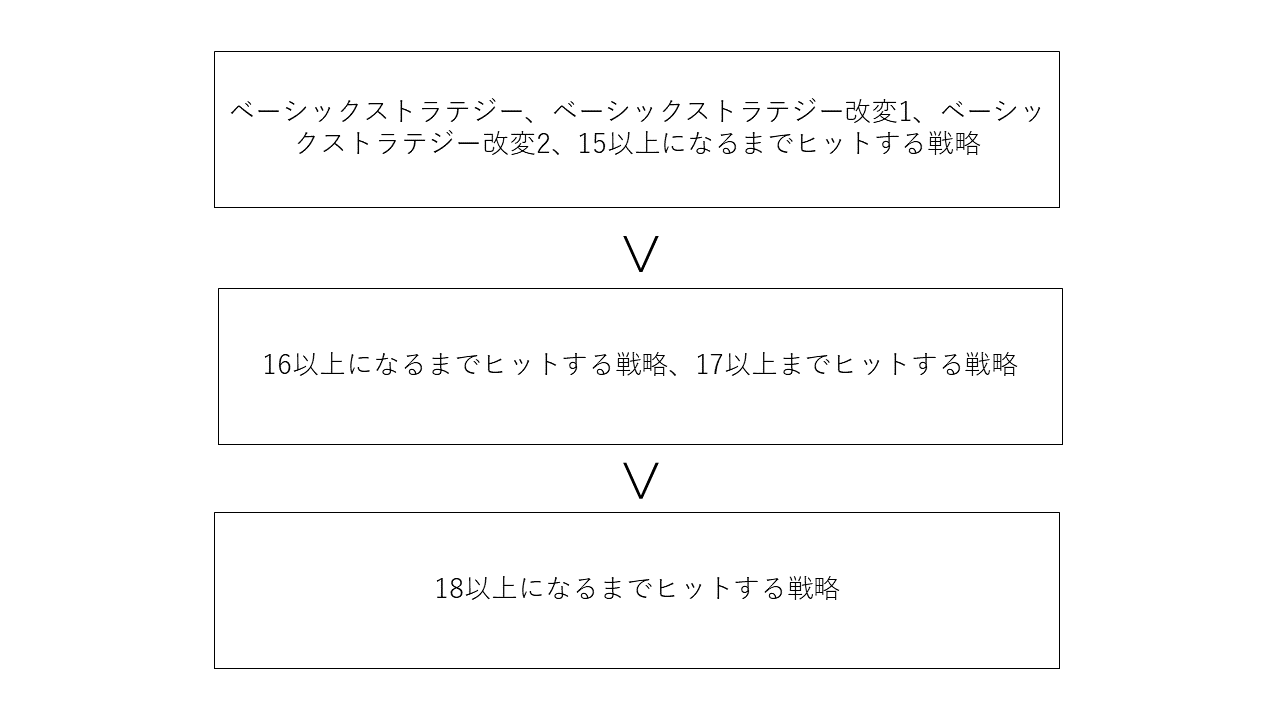
\includegraphics[width=0.7\linewidth]{./figure/statistics-rate1}
  \caption{デック数無限の勝率順\label{rate1}}
 \end{center}
\end{figure}

デック数1の場合、ベーシックストラテジー、ベーシックストラテジー改変1とベーシックストラテジー改変2の3つに勝率に有意な差が存在しない。15以上になるまでヒットする戦略、16以上になるまでヒットする戦略と18以上になるまでヒットする戦略の3つに有意な差が存在しない。これらを勝率の高い順に戦略を並べると、ベーシックストラテジーとベーシックストラテジー改変1ベーシックストラテジー改変2の戦略、15と16と18以上になるまでヒットする戦略、17以上になるまでヒットする戦略となる。これを図\ref{rate2}で示す。

\begin{figure}[H]
 \begin{center} 
  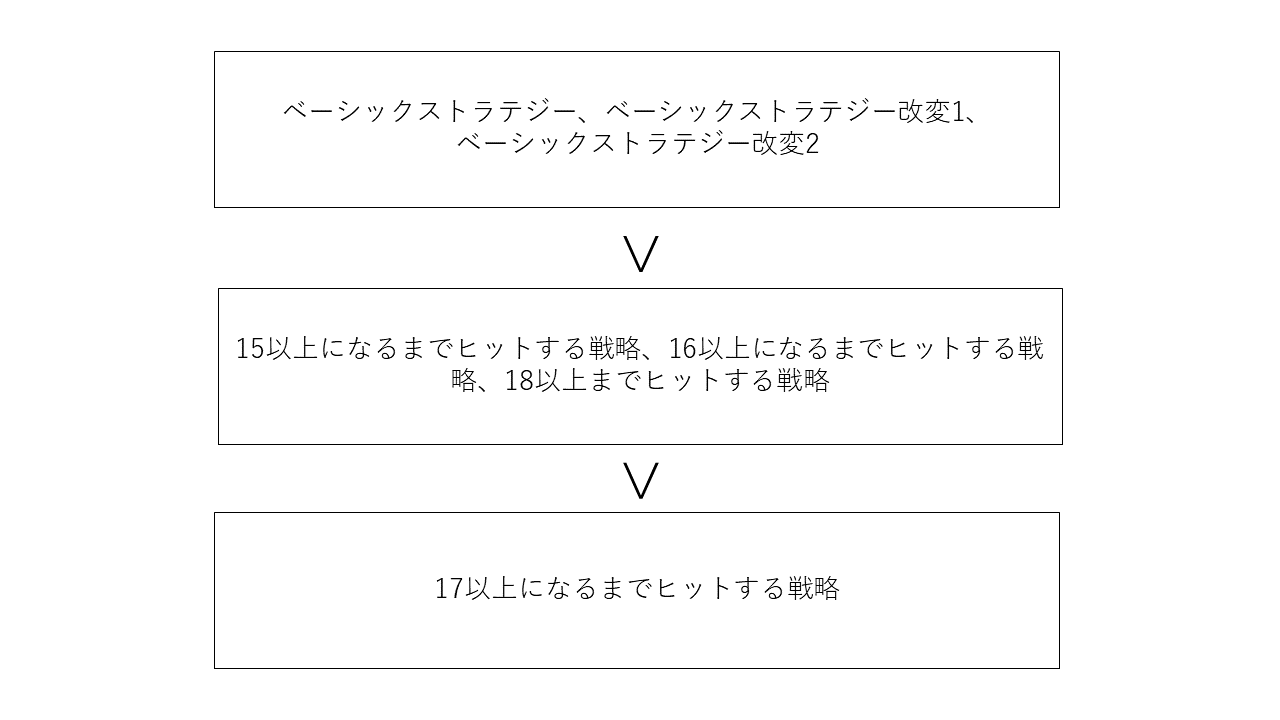
\includegraphics[width=0.7\linewidth]{./figure/statistics-rate2}
  \caption{デック数1の勝率順\label{rate2}}
 \end{center}
\end{figure}

\bunseki{柿崎大輝}

\section{複雑性を考慮した性能比較とその結果}

\subsection{各戦略の性能評価}

今回はシミュレーションから得た各戦略の勝率と定義した複雑性を用いて、各戦略の性能比較を行った。
性能の基準は以下の二通りを用意した。\\
~~ 性能1. (勝率) ÷ (複雑性)\\
~~ 性能2. (勝率) - (複雑性)\\
この評価基準に従って、デック数1の時の性能を表\ref{table:data_type4}、デック数無限の時の性能を表\ref{table:data_type5}にまとめた。

%\begin{table}[H]
%\caption{デック数1の時の各戦略の性能}
%\label{table:data_type4}
%\begin{center}
%\begin{tabular}{|c|c|c|c|c|c|}
%\hline
%戦略           & 圧縮長 & 勝率    & 複雑性   & 性能1  & 性能2   \\ \hline
%ベーシックストラテジー         & 30  & 0.431 & 0.375 & 1.14 & 0.052 \\ \hline
%ベーシックストラテジー改変1      & 28  & 0.429 & 0.35  & 1.22 & 0.076 \\ \hline
%ベーシックストラテジー改変2      & 26  & 0.430 & 0.325 & 1.21 & 0.072 \\ \hline
%15以上になるまでヒットする戦略 & 16  & 0.421 & 0.200 & 2.12 & 0.224 \\ \hline
%16以上になるまでヒットする戦略 & 16  & 0.416 & 0.200 & 2.07 & 0.214 \\ \hline
%17以上になるまでヒットする戦略 & 16  & 0.410 & 0.200 & 2.05 & 0.209 \\ \hline
%18以上になるまでヒットする戦略 & 16  & 0.421 & 0.200 & 1.97 & 0.193 \\ \hline
%\end{tabular}
%\end{center}
%\end{table}

%\begin{table}[H]
%\caption{デック数無限の時の各戦略の性能}
%\label{table:data_type5}
%\begin{center}
%\begin{tabular}{|c|c|c|c|c|c|}
%\hline
%戦略           & 圧縮長 & 勝率    & 複雑性   & 性能1  & 性能2   \\ \hline
%ベーシックストラテジー         & 30  & 0.427 & 0.375 & 1.14 & 0.052 \\ \hline
%ベーシックストラテジー改変1      & 28  & 0.424 & 0.35  & 2.12 & 0.224 \\ \hline
%ベーシックストラテジー改変2      & 26  & 0.414 & 0.325 & 1.07 & 0.214 \\ \hline
%15以上になるまでヒットする戦略 & 16  & 0.424 & 0.200 & 2.05 & 0.209 \\ \hline
%16以上になるまでヒットする戦略 & 16  & 0.414 & 0.200 & 1.97 & 0.193 \\ \hline
%17以上になるまでヒットする戦略 & 16  & 0.409 & 0.200 & 1.21 & 0.076 \\ \hline
%18以上になるまでヒットする戦略 & 16  & 0.393 & 0.200 & 1.21 & 0.072 \\ \hline
%\end{tabular}
%\end{center}
%\end{table}

\begin{table}[H]
\caption{デック数1の時の各戦略の性能}
\label{table:data_type4}
\begin{center}
\begin{tabular}{|c|c|c|c|c|c|}
\hline
戦略           & 圧縮長 & 勝率    & 複雑性   & 性能1  & 性能2   \\ \hline
ベーシックストラテジー         & 26  & 0.431 & 0.325 & 1.33 & 0.106 \\ \hline
ベーシックストラテジー改変1      & 24  & 0.429 & 0.300  & 1.43 & 0.129 \\ \hline
ベーシックストラテジー改変2      & 22  & 0.430 & 0.275 & 1.56 & 0.155 \\ \hline
15以上になるまでヒットする戦略 & 16  & 0.421 & 0.200 & 2.11 & 0.221 \\ \hline
16以上になるまでヒットする戦略 & 16  & 0.416 & 0.200 & 2.08 & 0.216 \\ \hline
17以上になるまでヒットする戦略 & 16  & 0.410 & 0.200 & 2.05 & 0.210 \\ \hline
18以上になるまでヒットする戦略 & 16  & 0.421 & 0.200 & 2.11 & 0.221 \\ \hline
\end{tabular}
\end{center}
\end{table}

\begin{table}[H]
\caption{デック数無限の時の各戦略の性能}
\label{table:data_type5}
\begin{center}
\begin{tabular}{|c|c|c|c|c|c|}
\hline
戦略           & 圧縮長 & 勝率    & 複雑性   & 性能1  & 性能2   \\ \hline
ベーシックストラテジー         & 26  & 0.427 & 0.325 & 1.31 & 0.102 \\ \hline
ベーシックストラテジー改変1      & 24  & 0.424 & 0.300  & 1.41 & 0.124 \\ \hline
ベーシックストラテジー改変2      & 22  & 0.414 & 0.275 & 1.51 & 0.139 \\ \hline
15以上になるまでヒットする戦略 & 16  & 0.424 & 0.200 & 2.12 & 0.224 \\ \hline
16以上になるまでヒットする戦略 & 16  & 0.414 & 0.200 & 2.07 & 0.214 \\ \hline
17以上になるまでヒットする戦略 & 16  & 0.409 & 0.200 & 2.05 & 0.209 \\ \hline
18以上になるまでヒットする戦略 & 16  & 0.393 & 0.200 & 1.97 & 0.193 \\ \hline
\end{tabular}
\end{center}
\end{table}

各戦略を比較し、次のような結果を得た。
勝率のみを考慮した場合、一定の数字以上になるまでヒットする戦略よりも、ベーシックストラテジーとそれを改変した戦略の方が有意に高い勝率だった。
ベーシックストラテジーと改変1、改変2のそれぞれの戦略間には有意な差が見られなかった。
複雑性を考慮して性能を評価した場合、デック数1の時は15以上になるまでヒットする戦略と、18以上になるまでヒットする戦略が最も性能が良かった。デック数無限の時は、15以上になるまでヒットする戦略が最も性能が良かった。


\bunseki{渡邊凛}

\section{検証結果のまとめ}
これまで行った検証や性能評価による結果をまとめる。

勝率のみを考慮した場合
\begin{itemize}
\item 結果1:一定の数字以上になるまでヒットする戦略よりも、ベーシックストラテジーとベーシックストラテジー改変1、ベーシックストラテジー改変2のほうが有意に高い勝率だった
\item 結果2:ベーシックストラテジーとベーシックストラテジー改変1、ベーシックストラテジー改変2のそれぞれの戦略間に有意な差はみられなかった
\item 結果3:ベーシックストラテジー改変1と18以上までヒットする戦略にはデック数無限とデック数1で勝率に有意な差があった
\end{itemize}

勝率を考慮すると、ベーシックストラテジーとベーシックストラテジー改変1、ベーシックストラテジー改変2の3つが勝率が高く、優秀な戦略であることが分かった。ただ、ベーシックストラテジー改変1はデック数の違いによって勝率に差がある。

複雑性を考慮して性能を評価した場合
\begin{itemize}
\item 結果4:15以上になるまでヒットする戦略が1番優秀であることが判明した
\end{itemize}

複雑性を考慮すると、ベーシックストラテジーには改善の余地があることが判明した。
\bunseki{柿崎大輝}
\section{賭け金の導入}
ここまでのシミュレーションでは主に勝率について考えてきた。しかし、ブラックジャックで重要なのは勝率ではなく、勝ってお金を増やすことが最も重要である。そのため、ここからのシミュレーションではお金を賭けて勝負を行い、お金がどのように増減するのかに注目していく。
\bunseki{※柿崎大輝}
\subsection{一定ベット}
まずは、賭け金を常に一定として、所持金がどのように変化するのかをシミュレーションで調べる。このシミュレーションでは最初の所持金を1000とし、常に10賭け、勝負を連続で40回行う。これを50000セット行う。また戦略はダブルダウンやスプリットなどが入ったベーシックストラテジー(BS)とヒットとスタンドのみのベーシックストラテジー(BS-HS)、GAで作成した戦略(GA戦略)の3つを使用する。シミュレーション結果を図\ref{betdife}と表\ref{bet}で示す。
\begin{figure}[H]
 \begin{center} 
  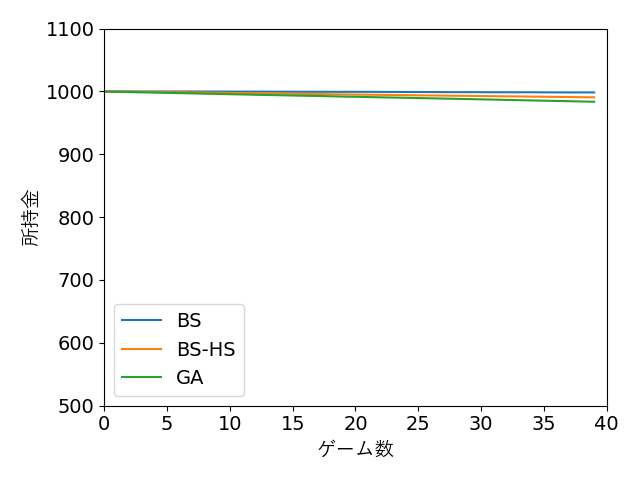
\includegraphics[width=0.7\linewidth]{./figure/bet-defineite-ver5}
  \caption{一定ベット\label{betdife}}
 \end{center}
\end{figure}

\begin{table}[H]
 \caption{一定ベットの所持金\label{bet}}
 \begin{center}
  \begin{tabular}{|c|c|c|}
  \hline  & 40回目の平均所持金 & 標準偏差 \\
  \hline BS & 998.328 & 73.538\\
  \hline BS-HS & 990.499 & 62.013 \\
  \hline GA戦略 & 983.470 & 62.401\\
  \hline
  \end{tabular}
 \end{center}
\end{table}

図\ref{betdife}では所持金は勝負を重ねるたびに少しずつ少なくなっていて、最後の40回目では最初の所持金である1000より少し少なくなっているように見える。そこで表\ref{bet}を見ると40回目のそれぞれの所持金が分かるが、ベーシックストラテジー、ヒットスタンドのみのベーシックストラテジー、GA戦略の順で多いことが分かる。どの戦略でも最初の所持金である1000を超えることはないことが分かった。\\
 賭け金が一定では最初の所持金を超えることができなかった。そのため賭け金を変動させることが必要だと考えた。まず、この勝負40回の中で勝率が変動するところがないかを確認した。勝負のどこかで勝率が高くなれば賭け金をあげ、低くなれば賭け金を下げることで所持金を増やそうと考えたためである。また、カウンティングという手法を用いてみるという2つの手法を考えた。
\bunseki{※柿崎大輝}

\subsection{勝率の推移}
ブラックジャックを連続で行った場合で勝率は変化するのかを調べる。ブラックジャックは連続で40回行い、その40回すべての勝率を調べる。使用した戦略はヒットスタンドのみのベーシックストラテジーを使用した。デック数は6とした。この条件で5万回行った。シミュレーション結果を図\ref{win}で示す。
\begin{figure}[H]
 \begin{center} 
  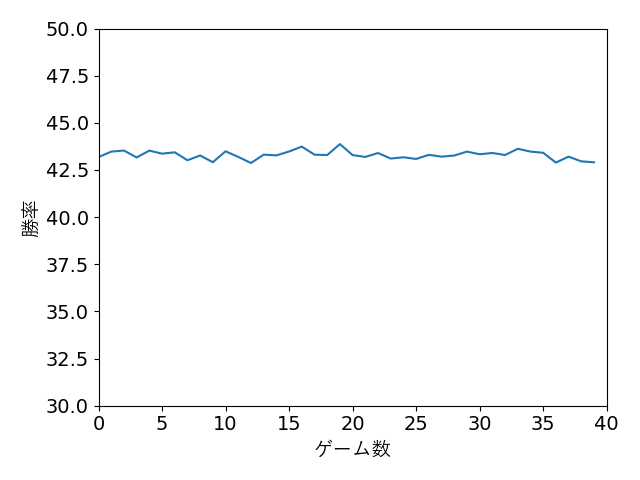
\includegraphics[width=0.7\linewidth]{./figure/win}
  \caption{カウンティングKO法\label{win}}
 \end{center}
\end{figure}
図\ref{win}を見ると勝率は42\%~44\%の間で増減を繰り返しており、だいたい43\%の部分に集中していると分かる。勝率は特に目立った規則性は見られず、ランダムに増減を繰り返しているように見られる。勝率は最高で43.87\%で最低は42.868\%であった。
 シミュレーション結果から勝率は勝負40回の中であまり変化しないと考えられる。また、勝率の変動に規則性は見つからなかった。そのため、勝負のどこかで賭け金を増やすという戦略はできないということが分かった。
\bunseki{※柿崎大輝}

\subsubsection{カイ2乗検定}
個々の勝負での勝率での差は小さいものであった。しかし、本当にその差には意味がないのか、小さくても本当は意味がある差なのではないか。それを確かめるために、カイ2乗検定を行い、勝率の差が有意な差であるかどうかを確かめる。
 帰無仮説は勝率の差に有意な差はない。対立仮説は勝率の差に有意な差があるとし、有意水準5\%で行った。表\ref{win-x}でこの条件についてまとめた。
\begin{table}[H]
 \caption{勝率の差のカイ2乗検定条件\label{win-x}}
 \begin{center}
  \begin{tabular}{|c|c|}
  \hline 帰無仮説 & 勝率の差に有意な差がない \\
  \hline 対立仮説 & 勝率の差に有意な差がある \\
  \hline 有意水準 & 5\% \\
  \hline
  \end{tabular}
 \end{center}
\end{table}
カイ2乗検定を行うとカイ2乗値は40.207となった。この値をp値に変換すると54.57。p値が0.05以上となったので帰無仮説を採択する。よって勝率の差には有意な差がないという結果になった。つまり、勝負40回で勝率の変化はないという結果となる。
\bunseki{※柿崎大輝}

\subsection{カウンティング}
カウンティングで賭け金を変動させ、所持金を調べる。カウンティングはKO法とHigh-Low法の2種類を用いる。そのほかの条件は一定ベットの時のシミュレーションと同じとした。シミュレーション結果を図\ref{KO}と図\ref{Hi-Lo}と表\ref{countting}で示す。
\begin{figure}[H]
 \begin{center} 
  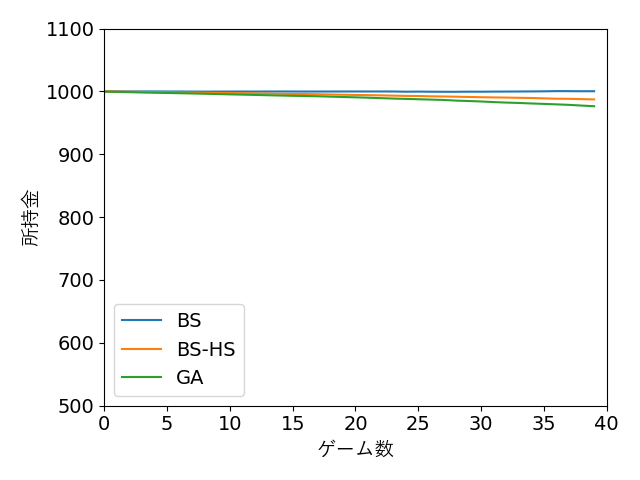
\includegraphics[width=0.7\linewidth]{./figure/KO}
  \caption{カウンティングKO法\label{KO}}
 \end{center}
\end{figure}

\begin{figure}[H]
 \begin{center} 
  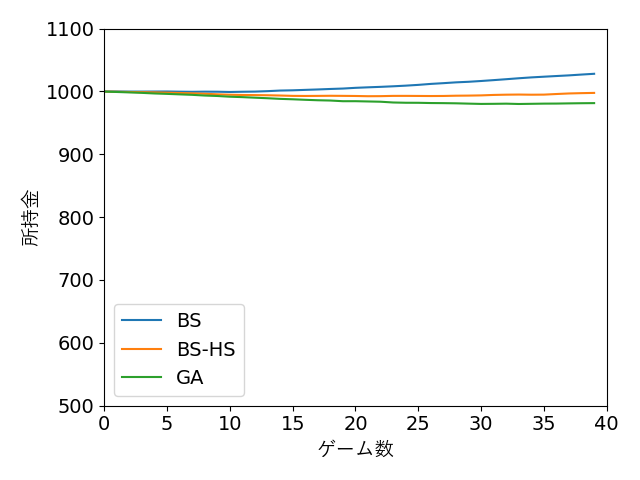
\includegraphics[width=0.7\linewidth]{./figure/Hi-Lo}
  \caption{カウンティングHigh-Low法\label{Hi-Lo}}
 \end{center}
\end{figure}

\begin{table}[H]
 \caption{カウンティングの所持金\label{countting}}
 \begin{center}
  \begin{tabular}{|c|c|c|}
  \hline  & 40回目の平均所持金 & 標準偏差 \\
  \hline KO法BS & 1000.237 & 172.770\\
  \hline KO法BS-HS & 987.207 & 148.615 \\
  \hline KO法GA戦略 & 976.380 & 145.821\\
  \hline High-Low法BS & 1027.961 & 298.197\\
  \hline High-Low法BS-HS  & 997.561 & 262.546\\
  \hline High-Low法GA戦略 & 981.315 & 263.162\\
  \hline
  \end{tabular}
 \end{center}
\end{table}

図\ref{KO}でKO法を見ると一定ベットの時とあまり変化がないように見えるが、表\ref{countting}で見るとベーシックストラテジーの所持金が増加していることが分かる。図\ref{Hi-Lo}のHigh-Low法ではで増えていることがはっきりと分かる。表\ref{countting}で見てもすべての戦略で一定ベットの時よりも増えていることが分かる。しかし、標準偏差が一定ベットやKO法の2つより大きく、安定していないことが分かる。カウンティングを使うことでベーシックストラテジーでは1000を超えることができた。ただ、ヒットスタンドのみのベーシックストラテジーやGA戦略では1000を超すことはできなかった。\\
 ここで注目するのはGA戦略である。一定ベットやカウンティングを使用しても所持金がすべての戦略で一番少なかった。GA戦略は遺伝子アルゴリズムで探索し、発見した戦略であるのになぜ他の戦略より悪い結果となったのか。それは複雑性ということを考慮していないからではないかと考えた。GA戦略は勝率と複雑性からなる性能で探索したもので、行ったシミュレーションでは複雑性を考慮する部分がなく、その結果一番悪い結果となったと考えた。そこで複雑性を確かめる実験の結果を用いて、"エラー率"という指標を作成し、シミュレーションに導入して行うこととした。
\bunseki{※柿崎大輝}

\subsection{エラー率}
エラー率を導入して、シミュレーションを行う。エラー率は戦略に従って行動するときにミスをする確率で、ミスをすると戦略表とは異なる行動を実行するようにした。それ以外の部分は前のシミュレーションと同じ条件とした。表\ref{err}が戦略ごとのエラー率で、図\ref{errKO}と図\ref{errHi-Lo}、表\ref{money-err}がシミュレーション結果である。
\begin{table}[H]
 \caption{戦略ごとのエラー率\label{err}}
 \begin{center}
  \begin{tabular}{|c|c|}
  \hline 戦略 & エラー率(\%) \\
  \hline BS & 16.2\\
  \hline BS-HS & 4.8 \\
  \hline GA戦略 & 0.5\\
  \hline
  \end{tabular}
 \end{center}
\end{table}

\begin{figure}[H]
 \begin{center} 
  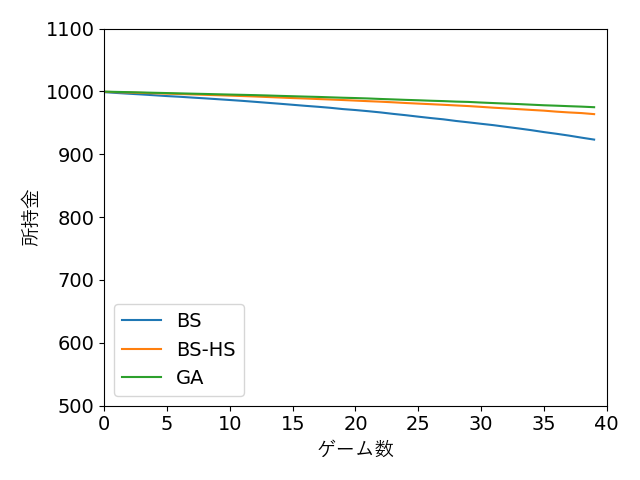
\includegraphics[width=0.7\linewidth]{./figure/errKO}
  \caption{エラー率ありのKO法\label{errKO}}
 \end{center}
\end{figure}

\begin{figure}[H]
 \begin{center} 
  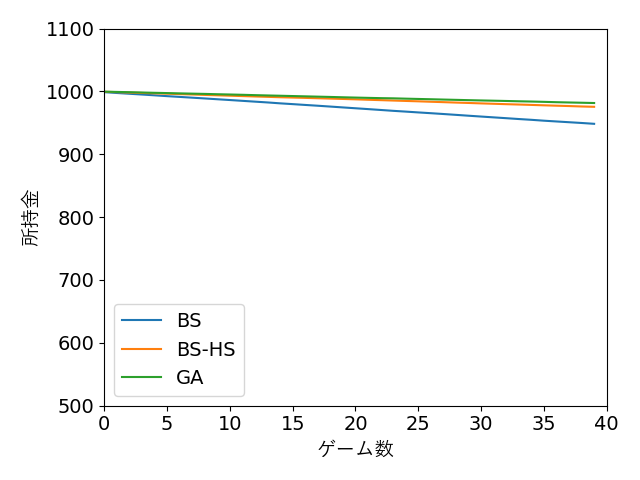
\includegraphics[width=0.7\linewidth]{./figure/errHi-Lo}
  \caption{エラー率ありのHigh-Low法\label{errHi-Lo}}
 \end{center}
\end{figure}

\begin{table}[H]
 \caption{エラー率を使用した際の所持金\label{money-err}}
 \begin{center}
  \begin{tabular}{|c|c|c|}
  \hline  & 40回目の平均所持金 & 標準偏差 \\
  \hline KO法BS & 923.303 & 174.255\\
  \hline KO法BS-HS & 963.799 & 150.135 \\
  \hline KO法GA戦略 & 974.817 & 144.821\\
  \hline High-Low法BS & 948.394 & 79.764\\
  \hline High-Low法BS-HS  & 975.440 & 67.263\\
  \hline High-Low法GA戦略 & 981.474 & 67.747\\
  \hline
  \end{tabular}
 \end{center}
\end{table}
エラー率を導入した結果ではGA戦略、ヒットスタンドのみのベーシックストラテジー、ベーシックストラテジーの順となり、所持金が1番多かったベーシックストラテジーと1番少なかったGA戦略が入れ替わった。特にベーシックストラテジーはエラー率を導入することで大きく所持金が少なくなった。またエラー率を導入したシミュレーションでは1000を超える戦略はないことが分かった\\
 エラー率を導入した場合、GA戦略が1番優れていることが分かった。しかし、GA戦略では1000を超えることができないことも分かった。この点にGA戦略は改善がする必要があると考えられる。
\bunseki{※柿崎大輝}

\subsubsection{分散分析}
エラー率を導入したシミュレーションの時、3つの戦略間で40回目の平均所持金に有意な差があるかどうかを調べる。まず、3つの戦略において有意な差があるかどうかを調べるため、分散分析を行った。優位水準は5\%、KO法とHigh-Low法の2種類で行った。表\ref{conditions-b}で分散分析の条件をまとめた。
\begin{table}[H]
 \caption{分散分析の条件\label{conditions-b}}
 \begin{center}
  \begin{tabular}{|c|c|}
  \hline 帰無仮説 & 3つの戦略で平均所持金に有意な差はない \\
  \hline 対立仮説 & 3つの戦略で平均所持金に有意な差はある \\
  \hline 有意水準 & 5\% \\
  \hline
  \end{tabular}
 \end{center}
\end{table}
分散分析を行うと、KO法、High-Low法のp値がとても小さくなり、0.05以下となる。よって帰無仮説を棄却し、対立仮説を採択する。つまり、3つの戦略で有な差が存在することが確認できた。次は3つの戦略のどこに有意な差が存在するのかを調べるためにここから多重比較を行う。
\bunseki{※柿崎大輝}

\subsubsection{多重比較}
それぞれの戦略で有意な差があるかを調べため、多重比較を行った。有意水準を5\%として行った。結果は表\ref{multiKO}と表\ref{multiHigh-Low}に示す。
\begin{table}[H]
 \caption{KO法での多重比較\label{multiKO}}
 \begin{center}
  \begin{tabular}{|c|c|c|}
  \hline  & BS & BS-HS  \\
  \hline  BS-HS 所持金の差 & 40.496 & \\
	               p値 & 0 & \\
  \hline GA 所持金の差 & 51.515 & 11.019\\
                p値 & 0 & 0\\
  \hline
  \end{tabular}
 \end{center}
\end{table}
\begin{table}[H]
 \caption{KO法での多重比較\label{multiHigh-Low}}
 \begin{center}
  \begin{tabular}{|c|c|c|}
  \hline  & BS & BS-HS  \\
  \hline  BS-HS 所持金の差 & 27.046 & \\
	               p値 & 0 & \\
  \hline GA 所持金の差 & 33.080 & 6.034\\
                p値 & 0 & 0\\
  \hline
  \end{tabular}
 \end{center}
\end{table}
 KO法ではすべての戦略間でp値が0.05以下となり、すべての戦略間で有意な差が存在することが分かった。High-Low法でもすべての戦略間でp値が0.05以下となり、すべての戦略間で有意な差が存在することが分かった。これでKO法High-Low法の両方ですべて戦略間で有意な差が存在する。
\bunseki{※柿崎大輝}
\chapter{前期活動}
本プロジェクトで題材としているブラックジャックというゲームを
実際のプレイも交えて学習した。前章までで説明したベーシックストラテジーを
試すということもその中で行ったが、実際に使用してみると表を覚え、かつ
素早いゲームの進行に合わせながら実行するのは容易ではないという実感が得られた.
もちろんディーラー側に戦略の実行をさとられないようにするためには、ゲームの進行を
止めるなど違和感を持たせるような行動はできるだけ無くす必要がある。以上のことから、
戦略の単純化の必要性を再確認した。

シミュレータはPython3で作成を行った。前期までで得られたブラックジャックの戦略比較に用いた
数値はこのシミュレータによって得られた。また開発の効率化のためにバージョン管理システムである
Gitを導入し、Gitによるバージョン管理について学習した。

シミュレータの正しさ、シミュレーション結果の分析のために統計学を学習した。

本プロジェクトにおいて、戦略の複雑性を評価することはとても重要な事項である。
複雑性の定義付けのためにChaitin(1969)によって定義されたコルモゴロフ複雑性の定義を参考にし、コルモゴロフ複雑性の定義と使われ方について調査し学習した。

本プロジェクトでは最適な戦略の探索を行うための技術の一つとしてニューラルネットワークを挙げ、斎藤(2016) の書籍を教科書とし、勉強会を行った。

\bunseki{米村祥裕}


%\chapter{後期目標}
%後期の目標としては次が挙げられる。

\begin{itemize}
\item ディーラー側の行動の検証
\item デックが有限個の場合での戦略
\item 賭け金の概念の導入
\item より扱いやすい戦略の検証
\end{itemize}

ディーラー側の行動の検証については、ニューラルネットワークを用いて、プレイヤーがどのような戦略を取っているのかを検知するプログラムを作成することを目標にしている。例えば、プレイヤーがカウンティング戦略を使用している際にそれを見抜く事ができるようなプログラムを作成し、そうして作成したプログラムを用いて、ディーラー側に検知されにくい戦略の生成に活用しようと考えている。

デックが有限個の場合での戦略については、実際の対戦に従って、デック数が有限でシャッフルを一定ゲーム数まで行わず、連続でゲームを行う場合の最適な戦略を検証することを目標にしている。前述したとおりベーシックストラテジーはデック数が無限であるという前提のもと成立している戦略であるが、実際のゲームにおいてはデック数は有限であり、シャッフルを一定ゲーム数まで行わない。この事から、ゲームの進行状況により、最適とされる戦略が変わる可能性がある。そのため、デック数が有限で連続してゲームを行うと設定した状態での最適な戦略について検証することを考えている。

賭け金の概念の導入では実際のブラックジャックのゲームに則って賭け金を設定し、利得をどの様にプラスにしていくか、そのための最適な行動を考える。前期の活動では賭け金の概念は考えず、戦略の勝率のみに着目していた。しかし、実際のブラックジャックのゲームにおいては戦略の勝率が低かったとしても賭け金の賭け方によっては利得をプラスにすることが可能である。この事から、戦略の勝率のみに着目するのではなく、賭け金の賭け方にも着目し、最終的な利得をプラスにしていく戦略を検証することを考えている。

より扱いやすい戦略の検証について、今回は複雑性の設定を手動で行い、検証する時間もあまり取らなかったため、評価基準が正確ではない可能性がある。今後、この評価基準をどのように調整するかも検討しようと考えている。

\bunseki{※渡邊凛}
\chapter{後期活動}
後期は、まず主に3つの課題を設定し、それぞれの課題解決に向かってグループを作成し活動した。

1つ目の課題は、遺伝的アルゴリズムを使用して新しいブラックジャックの戦略を探索することである。以下、この課題解決を行ったグループ名を、GA班とする。

2つ目の課題は、前期活動で設定した複雑性という要素が、人間が戦略表を記憶する能力と一致しているのかを、実験を通して検証することである。以下、この課題解決を行ったグループ名を、複雑性班とする。

3つ目の課題は、最適な戦略の探索に、賭け金の概念を導入し、それに伴いカウンティングについても既存のものを学習し、賭け方に考慮することである。以下、この課題解決を行ったグループ名を、カウンティング班とする。

以下に、それぞれのグループの活動のあらましを述べる。

\begin{itemize}
\item GA班
\end{itemize}

まずはじめに、遺伝的アルゴリズムを用いて戦略を探索するプログラムを作成した。遺伝的アルゴリズムを使用した背景には、ブラックジャックの戦略の組み合わせは膨大であり、遺伝的アルゴリズムを使用するのが最適であると判断したという理由がある。使用した言語はPythonである。探索は、研究費で購入した計算用PCを使用し、また学内から接続できるようにネットワーク設定も行った。

そのようにして得られた戦略を用いて勝率を導出したが、予想されていたほどの結果は出なかった。そこで原因を解明したところ、交叉手法や突然変異確率、初期個体値の見直しが必要であると判明した。それらを見直したうえで最終的にGA戦略という新たな戦略を導出した。

\begin{itemize}
\item 複雑性班
\end{itemize}

まずはじめに、コルモゴロフ複雑性を参考にし、複雑性とカウンティングなどの戦略の組み合わせで利得が最大になるような戦略の評価方法を考えた。

その結果、戦略の評価方法を知るには実際に人間に戦略表を記憶させる実験を行うことが必要だと判明したため、実験の計画をたてた。実験には認知的判断能力も知る必要があったため、知能テストの作成も行った。

実験から得られた結果をもとに、前期に作成した複雑性との相関を検定した。その結果、2つの間には非常に強い負の相関がみられた。つまり、複雑性が高くなるにつれ、戦略表を間違えて覚えやすいということであり、我々が導出した複雑性は評価指標として適していることが明らかになった。

また、同時に行った認知的判断能力テストの結果から、ブラックジャックの戦略を記憶するうえで一般的な認知能力は関係がないという新しい結果も得られた。

\begin{itemize}
\item カウンティング班
\end{itemize}

まずはじめに、前期に作成したシミュレータを改変し、ダブルダウン、スプリット、サレンダーが行えるようにした。それに伴い、それらのルールを織り込んだカウンティングとベッティングシステムについて調査した。ベッティングシステムについては、それぞれの比較が必要であったため、比較方法の手法の検討も行った。

これらの研究から、ある戦略を使用した際、膨大な数のゲーム数を行った場合の最終的な利得を、カウンティング手法を変更した時でも導出できるシミュレータの開発に成功した。そしてこのシミュレータを使用して、GA班が導出した戦略について検証した。

ところがGA班から導出された戦略を用いた戦略では、基本戦略を超えた結果が出ることはなかった。これについて検討したところ、戦略を間違えて覚える確率(以下、エラー率とする)について考えていなかったためそのような結果になったと考えられた。そこで、複雑性班が行った実験の結果を基にエラー率を導出し、シミュレーションに組み込んだ。その結果、当初の予想の通り、GA班が導出した戦略が一番優秀であるという結果が得られた。

\begin{itemize}
\item 共通して行った事
\end{itemize}

函館市の高校生が参加する見学会があったため、そのためのスライド作成などを行った。
12月には、一年の活動の総まとめとして成果発表会に参加した。

\bunseki{菱田美紗紀}

\chapter{中間発表の評価}
 本章では中間発表で記入してもらった評価シートの集計結果とコメントを参考にして今後の改善点を記述する。
 評価シートの評価項目は「発表技術」と「発表内容」の2つと「発表内容」の細部に「ブラックジャックのルール説明の評価」、「検証の評価」の2つ合わせて計4つ用意した。そして、それぞれについて1(非常に悪い)から10(非常に優秀)までの間で評価点を付け、それぞれについてのコメント(評価理由)やアドバイスを記入する欄を用意した。
\bunseki{葛西隼人}
\section{中間発表}
\subsection{評価点数の集計}
中間発表で記入してもらった評価シートは計42枚だった。シートを記入した人の所属の分布の表\ref{tab:dist} のようになった。

\begin{table}[htb]
  \begin{center}
    \caption{評価人数集計}
    \begin{tabular}{|c|c|c|} \hline 
      所属 & 学年 & 人数  \\ \hline \hline
      教員 &  & 6  \\
      一般 &  & 0 \\
      学生 & 院2年 & 0 \\
     学生 & 院1年 & 0 \\
             & 学部4年 & 1 \\
       & 学部3年 & 34 \\
             & 学部2年 & 1 \\
             & 学部1年 & 0 \\ \hline \hline
      合計 &  & 42 \\ \hline
    \end{tabular}
    \label{tab:dist}
  \end{center}
\end{table}

評価人数の構成としては学部3年が大半を占めていた。その他には教員、学部4年と学部1年から1
人ずつであった。次はそれぞれの評価項目についての平均点を表\ref{tab:point}に記す。

\begin{table}[H]
\begin{center}
\caption{評価点数集計}
\begin{tabular}{|c|c|c|c|c|c|} \hline
  所属 & 学年 & 発表技術 & 発表内容 & ルール説明 & 検証説明  \\ \hline \hline
  教員 &        & 8 & 7.5 & 7.83 & 7.67 \\
  学生 &        & 6.47 & 7.03 & 7.56 & 6.22 \\
         & 学部2,4年 & 6 & 7 & 5.5 & 7 \\
         & 学部3年 & 6.38 & 7.01 & 7.68 & 6.18 \\ \hline \hline
  全体 &        & 6.69 & 7.1 & 7.6 & 6.43 \\ \hline
\end{tabular}
\label{tab:point}
\end{center}
\end{table}

全体の平均は「発表技術」については6.69、「発表内容」については7.1、「ルール説明」については7.6、「検証説明」については6.43となった。それぞれの項目について高く評価したのは「教員」だった。
次に、それぞれの結果を図\ref{evaluation-gizyutu}、図\ref{evaluation-naiyou}、図\ref{evaluation-ru-ru}、図\ref{evaluation-kensyou}に示す。

\begin{figure}[h]
 \begin{tabular}{cc}
  \begin{minipage}[h]{0.45\hsize}
  \centering
 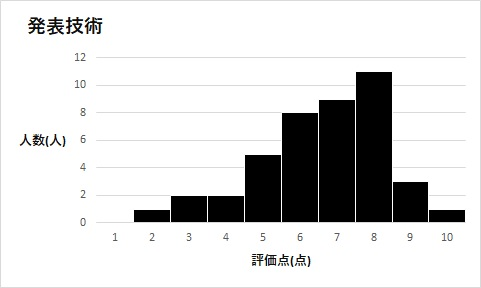
\includegraphics[width=0.7\linewidth]{./figure/evaluation-gizyutu.jpg}
\caption{発表技術の評価グラフ}
\label{evaluation-gizyutu}
 \end{minipage} &

\begin{minipage}[h]{0.45\hsize}
  \centering
 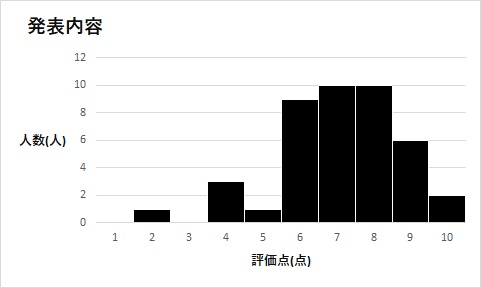
\includegraphics[width=0.7\linewidth]{./figure/evaluation-naiyou.jpg}
 \caption{発表内容の評価グラフ}
\label{evaluation-naiyou}
\end{minipage} 
\end{tabular}
\end{figure}

\begin{figure}[h]
 \begin{tabular}{cc}
  \begin{minipage}[h]{0.45\hsize}
  \centering
 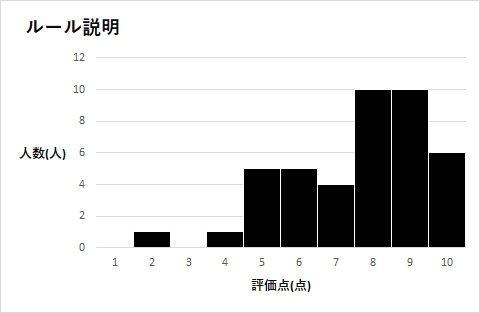
\includegraphics[width=0.7\linewidth]{./figure/evaluation-ru-ru.jpg}
\caption{ルール説明の評価グラフ}
\label{evaluation-ru-ru}
 \end{minipage} &

\begin{minipage}[h]{0.45\hsize}
  \centering
 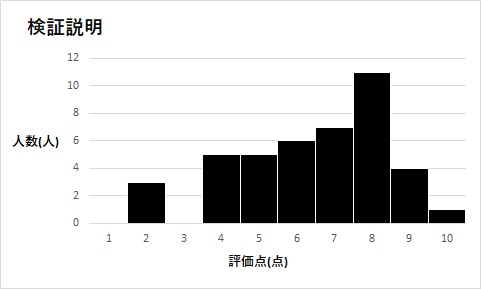
\includegraphics[width=0.7\linewidth]{./figure/kensyou.jpg}
 \caption{検証説明の評価グラフ}
\label{evaluation-kensyou}
\end{minipage} 
\end{tabular}
\end{figure}

「発表技術」と「発表内容」については評価点が共に7、8点と高い評価点が多かった。ルール説明についても同様に高い評価点が多かった、一方で検証説明については4、5点が多い結果となった。

また、「発表技術」と「発表内容」の評点の相関係数は0.71となった。これは2つの評価項目がかなり関連してると言える数値である。次にコメントについて解析する。
\bunseki{葛西隼人}

\subsection{コメント解析と改善点}
まず、「発表技術」について、肯定的なコメントと否定的なコメントに分けて並べる。

肯定的なコメント
\begin{itemize}
\item 複雑な内容をうまく説明してくれた
\item スライド内で図を多用されていて分かりやすかった
\end{itemize}

否定的なコメント
\begin{itemize}
\item 前を見て話してもらえないと聞き取りにくい
\item 説明が少し早い
\item プレゼンの内容が構造的でないために、全体に対して今どの部分を話しているのかわかりにくい
\end{itemize}

今回はスライドの分量が多く、どうしても早口になってしまったのでこのような意見が多かった。そしてスライドの完成が遅かったために構成までについて詳しく話し合うことができなかった。また発表の練習時間が取れなかったために技術面で足りない点もいくつかコメントで述べられていた。
次に、「発表内容」についても同様に、コメントを肯定的なコメントと否定的なコメントに分けて並べる。
肯定的なコメント
\begin{itemize}
\item 活動内容が明確でよかった
\item 実験・検証が多く、説得力をもたせている
\item 評価基準や比較対象が明確で理解しやすかった
\end{itemize}

否定的なコメント
\begin{itemize}
\item 用語についてより詳しく説明すべき
\item 聞く人の知識が必要になるのでもう少しわかりやすく
\item 検証結果のみせ方にもう少し工夫があると良かった。(専門的な知識がない人にもわかりやすく)
\end{itemize}

「発表内容」に関しては、ブラックジャックのルール説明はわかりやすいとのコメントが多かった。しかし検証の説明はあまり理解出来ないとのコメントも見受けられた。最後に「発表内容」と「発表技術」の2つのコメント欄から重要なアドバイスがいくつかあったため、これらについても述べていく。 
\begin{itemize}
\item なぜあのような式を利用することで性能が表されているかの説明がもう少し欲しかった
\item 文字数を減らし簡潔な内容の方がいいと思う
\item スライドに色を使って見やすくしたほうが良い
\item 基本的に文字がたくさんのスライドで、太字や下線などもなかったので、どこに注目してよいかわからなかった。後期の発表ではもっとスライドを効果的に見せてほしい
\end{itemize}
これらの意見に関しても、後期の活動に反映することとする。
以上より中間発表の評価コメントは賛否両論であり、とても参考になった。
\bunseki{葛西隼人}
\chapter{最終成果発表の評価}
 本章では最終成果発表で記入してもらった評価シートの集計結果とコメントを参考にして今後の改善点を記述する。
 評価シートの評価項目は「発表技術」と「発表内容」の2つと「発表内容」の細部に「複雑性についての説明の評価」、「カウンティングについての説明の評価」の2つ合わせて計4つ用意した。そして、それぞれについて1(非常に悪い)から10(非常に優秀)までの間で評価点を記入する欄、それぞれについてのコメント(評価理由)やアドバイスを記入する欄をそれぞれ用意した。
\bunseki{葛西隼人}
\section{最終成果発表}
\subsection{評価点数の集計}
最終成果発表で記入してもらった評価シートは計50枚だった。シートを記入した人の所属の分布は表\ref{tab:dist2} のようになった。

\begin{table}[htb]
  \begin{center}
    \caption{評価人数集計}
    \begin{tabular}{|c|c|c|} \hline 
      所属 & 学年 & 人数  \\ \hline \hline
      教員 &  & 7  \\
      一般 &  & 8 \\
      学生 & 院2年 & 0 \\
     学生 & 院1年 & 0 \\
             & 学部4年 & 0 \\
       & 学部3年 & 31 \\
             & 学部2年 & 2 \\
             & 学部1年 & 2 \\ \hline \hline
      合計 &  & 50 \\ \hline
    \end{tabular}
    \label{tab:dist2}
  \end{center}
\end{table}

中間発表では一般の評価人数が0人だったが、今回は函館市内の高校生が来ていたため一般の評価人数は増えて8人だった。学生と教員に関しては学部4年が0人となった代わりに、学部1年が0人となっていた点以外は中間発表とほとんど差異のない構成人数であった。次はそれぞれの評価項目についての平均点を表\ref{tab:point2}に記す。
\begin{table}[H]
\begin{center}
\caption{評価点数集計}
\begin{tabular}{|c|c|c|c|c|c|} \hline
  所属 & 学年 & 発表技術 & 発表内容 & 複雑性説明 & カウンティング説明  \\ \hline \hline
  教員 &        & 7.42 & 7.14 & 7.14 & 6.71 \\ 
  一般 &        & 7.38 & 7 & 6.12 & 6.75 \\
  学生 &        & 7 & 7.2 & 6.66 & 7.02 \\
         & 学部1,2年 & 6.5 & 6.25 & 6.5 & 6.5 \\
         & 学部3年 & 6.87 & 7.39 & 6.7 & 7.26 \\ \hline \hline
  全体 &        & 7 & 7.2 & 6.66 & 7.02 \\ \hline
\end{tabular}
\label{tab:point2}
\end{center}
\end{table}

全体の平均は「発表技術」については7点、「発表内容」については7.2点、「複雑性説明」については6.66点、「カウンティング説明」については7.02点となった。中間発表と最終成果発表で「発表技術」のみ比較を行う。中間発表では6.69点、最終成果発表では7点となった。点数のみの比較でも0.31点高くなっている。これは中間発表からの技術改善が見られていると考えられる。「発表内容」については中間発表と異なるので比較は行わない。次に、それぞれの結果を図\ref{evaluation_final-gizyutu2}、図\ref{evaluation_final-naiyou2}、図\ref{evaluation_final-hukuzatusei}、図\ref{evaluation_final-counting}に示す。

\begin{figure}[h]
 \begin{tabular}{cc}
  \begin{minipage}[h]{0.45\hsize}
  \centering
 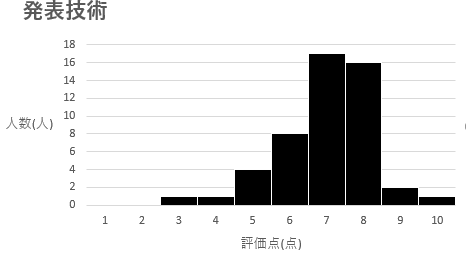
\includegraphics[width=0.7\linewidth]{./figure/evaluation_final-gizyutu2.jpg}
\caption{発表技術の評価グラフ}
\label{evaluation_final-gizyutu2}
 \end{minipage} &

\begin{minipage}[h]{0.45\hsize}
  \centering
 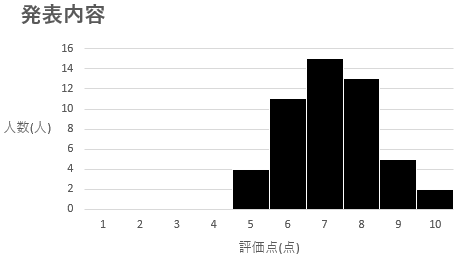
\includegraphics[width=0.7\linewidth]{./figure/evaluation_final-naiyou2.jpg}
 \caption{発表内容の評価グラフ}
\label{evaluation_final-naiyou2}
\end{minipage} 
\end{tabular}
\end{figure}

\begin{figure}[h]
 \begin{tabular}{cc}
  \begin{minipage}[h]{0.45\hsize}
  \centering
 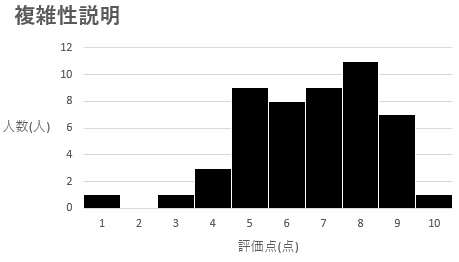
\includegraphics[width=0.7\linewidth]{./figure/evaluation_final-hukuzatusei.jpg}
\caption{複雑性説明の評価グラフ}
\label{evaluation_final-hukuzatusei}
 \end{minipage} &

\begin{minipage}[h]{0.45\hsize}
  \centering
 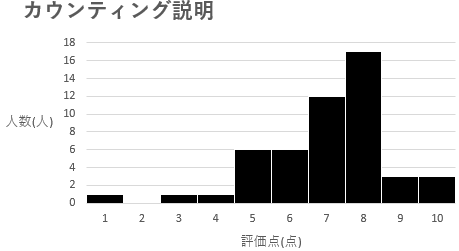
\includegraphics[width=0.7\linewidth]{./figure/evaluation_final-counting.jpg}
 \caption{カウンティング説明の評価グラフ}
\label{evaluation_final-counting}
\end{minipage} 
\end{tabular}
\end{figure}

「発表技術」と「発表内容」については評価点が共に7、8点と高い評価点が多かった。そして、「発表内容」に関しては最も低くても5点と全体的には評価はまとまっていたが、他のグラフは1,3
点など低い点数があり全体的な評価は散らばっていた結果となった。「複雑性説明」では5~8点の間にヒストグラムが集中していて理解度に差あることがわかった。

また、「発表技術」と「発表内容」の評価点数の相関係数は0.73となった。これは強い正の相関があり、2つの評価項目がかなり関連してると言える数値である。次にコメントについて解析する。
\bunseki{葛西隼人}

\subsection{コメント解析と改善点}
まず、「発表技術」について、肯定的なコメントと否定的なコメントに分けて並べる。

肯定的なコメント
\begin{itemize}
\item アニメーションがついてて見やすいスライドだと思った
\item アジェンダがあり、長いプレゼンがわかりやすかった
\item スライドの内容はよく整理されておりわかりやすかったです
\end{itemize}

否定的なコメント
\begin{itemize}
\item 発表場所が悪かったのもあり声がきこえないところがあった
\item 発表者が原稿を読んでいる感じがしたのが残念だった
\item 発表が単調で何が大事なポイントが分かりづらかった
\end{itemize}

スライド構成については評価するコメントはあったが、声が小さい、スライドの文字ばかり見ているとの発表者の技術面についての否定的な意見が多かった。そして発表の時間配分が他のプロジェクトと異なっていたため発表を全て聞けなかった人が少しいた。次に、「発表内容」についても同様に、肯定的なコメントと否定的なコメントに分けて並べる。

肯定的なコメント
\begin{itemize}
\item 仮説・実験・検証が適切に行われていた
\item 実験・検証が多く、説得力をもたせている
\item プロジェクト目標の設定が明確であった
\item 人間が使うことも含めた戦略の考察が面白いと思った
\end{itemize}

否定的なコメント
\begin{itemize}
\item エラー率は単純に複雑性から出すのではなく、似た状況がある時エラーするほうが正確なデータが出そうだと思った。
\item ポスターにもスライドにもチームとしてどう取り組んだのか全く示されていないのは、プロジェクト学習の発表として不十分に思えます
\end{itemize}

そして要望としてのあったコメントをいくつかあったので記述する。
\begin{itemize}
\item 勝率を100パーセントにしてほしい
\item 他のプロジェクトの発表もあるので、時間配分は考えてほしい
\end{itemize}

中間発表では、用語の説明が足りないというコメントが多く見受けられたが、最終成果発表ではカウンティングと複雑性の両方でわかりやすいというコメントがあった。今回の発表を通して得られた発表での留意点を以下に記述する。
\begin{itemize}
\item スライドは色を用いて見やすくする
\item 太線や下線などの重要な箇所を視覚的に理解できるようにする
\item 発表者は声は大きく、はっきり聞き取りやすく来ている人に目を向ける
\item 用語の説明を入れる、構成はアジェンダを用いてわかりやすくする
\end{itemize}

本プロジェクトでの中間発表と最終成果発表は今後の研究活動にも参考になる点が数多くあり非常に有益なものであった。
\bunseki{葛西隼人}
\chapter{今後の課題}
我々が一年を通して活動した結果、今後の課題は以下の2点であると判断した。

\begin{itemize}
\item 利得をプラスにできる戦略の探索
\item ブラックジャックをプレイする際に重要な能力の調査
\end{itemize}

このプロジェクトで最終的に一番優秀と判断された戦略を用いてシミュレーションをしたところ、最終的なプレイヤーの利得はマイナスであった。また、賭け金の賭け方からアプローチするため、High-Low法とKO法というカウンティング手法を、基本戦略、ヒットとスタンドのみの基本戦略、今回導出されたGA戦略の3つの戦略を用いて賭け金のシミュレーションを行ったが、いずれも利得がプラスになることはなかった。

我々のプロジェクトの目的は、ディーラーをやっつける、すなわちカジノ側から利益を得ることが大本の目的であるため、まだ目的を達成したとは言えない。

なぜこのような結果となったのか、我々の予想としては、今回の遺伝的アルゴリズムのシミュレーションにはエラー率という概念が導入されていないためと思われる。

複雑性は単にその戦略の複雑さを数値にしただけであるが、エラー率はそれに加え、人間がどれだけ戦略を間違えやすいかという要素が含まれている。

戦略の勝率を導出するために作成したシミュレータには、エラー率の概念が導入されているが、その戦略を探索する遺伝的アルゴリズムのプログラムには導入されていなかった。つまり、戦略を作成する段階と、その戦略を評価する段階で、評価指標が異なるものであったのである。そのため、作成段階では優秀とされた戦略が、評価するにあたって性能が良くないと判断されてしまったのである。

以上のことより、利得をプラスにするためには、勝率が50%以上の戦略を見つけだしゲームを行うか、カウンティングの手法を改変して利益を出すようにしなければならない。

そこで今後の課題として、遺伝的アルゴリズムにエラー率の概念を導入し、より勝率の高い戦略を見つけ出すことと、カウンティングの手法の中で優秀なものを、今回使用した遺伝的アルゴリズム、もしくは他の方法を用いて探索する事が挙げられた。

また、今回の複雑性の検証実験により、ブラックジャックをプレイする際、戦略表を記憶する上で、一般的な認知的判断能力は関係がないことがわかった。
つまり、別の指標を用いて、戦略表を記憶する能力を測ることができる可能性があるということである。
その能力とは何であるのかを調査することが2つ目の課題として挙げられた。

\bunseki{菱田美紗紀}


\begin{thebibliography}{20}
  \bibitem{blakjack2} Baldwin,R. and W. Cantey and H. Maisel and J. McDermott(1956) "The Optimum Strategy in Blackjack", {\it{Journal of the American Statistical Association}},vol.51, no.275, 419-439.
  \bibitem{complexity} Chaitin,G.J. (1969)"On the Simplicity and Speed of Programs for Computing Infinite Sets of Natural Numbers", {\it{Journal of the Association for Computing Machinery}}, vol.16, no.3, 407-422.
  \bibitem{strategiestable} Jensen, K. (2014)"The Expected Value of an Advantage Blackjack player" {\it{All Graduate Plan B and other Reports}}, 524.
  \bibitem{kelly} Kelly,J,L. (1956) "A New Interpretation of Infotnation Rate", {\it{THE BELL SYSTEM TECHNICAL JOURNAL}},vol35 , no.4, 917-926
  \bibitem{pythonDocument} Python Software Foundation(2018), "Python 3.6.5 ドキュメント", \verb|<|https://docs.python.jp/3/index.html\verb|>| 2018年7月1日アクセス.
  \bibitem{pythonrandom} Python Software Foundation(2018) "9.6. random - 擬似乱数の生成" \verb|<|https://docs.python.jp/3/ library/random.html\verb|>| 2018年6月20日アクセス
  \bibitem{basicstrategy} Thorp,E.(1962) {\it{Beat The Dealer:A Winning Strategy for the Game of Twenty One}},Vintage (宮崎三瑛(2006)『ディーラーをやっつけろ!』,パンローリング)
  \bibitem{KO} Vancura,O. and Fuchs,K.(1998) {\it{KNOCK-OUT BLACKJACK, HUNTINGTON PRESS}} (ライアン・モリス, 谷崎涼子(2012) 『カードカウンティング入門 - カジノでたのしむブラックジャックテクニック』, パンローリング)
  \bibitem{pairwise} 青木繁伸(2010) "比率の差の多重比較(pairwise.prop.test の拡張)" \verb|<|http://aoki2.si.gunma-u.ac.jp/R/p\_multi\_comp2.html\verb|>| 2018年7月21日アクセス
  \bibitem{ga} 北野宏明(1993)『遺伝的アルゴリズム』産業図書
  \bibitem{neuro2} 斎藤康毅 (2016) 『ゼロから作るDeep Learning Pythonで学ぶディープラーニングの理論と実装』森北出版株式会社
  \bibitem{blackjack1} 斎藤隆浩 (1999) 『新訂ブラックジャック必勝法』株式会社データハウス
 \bibitem{gaimprove} 佐藤浩,小野功,小林重信(1997) 『遺伝的アルゴリズムにおける世代交代モデルの提案と評価』,人工知能学会誌,12,5,pp.734-744
  \bibitem{zansa} 全人類がわかる統計学(2017) "カイ二乗検定を残差分析で評価する方法" \verb|<|https://to-kei.net/hypothesis-testing/chi2-test-residual-analysis/\verb|>| 2018年7月6日アクセス
  \bibitem{rway} 竹澤邦夫(2012) "19. 行列の作成" \verb|<|http://cse.naro.affrc.go.jp/takezawa/r-tips/r/19.html\verb|>| 2018年6月20日アクセス
  \bibitem{neuro1} 萩原将文 (1994) 『ニューロ・ファジィ・遺伝的アルゴリズム』産業図書株式会社
  \bibitem{random}広井誠(2007)"Algorithms with Python - 番外編:擬似乱数の検定" \verb|<|http://www.geocities.jp/m\_hiroi/light/pystat04.html\verb|>| 2018年6月20日アクセス
  \bibitem{mersenne} 松本眞(2013) "Mersenne Twister Home Page" \verb|<|http://www.math.sci.hiroshima-u.ac.jp/~m-mat/MT/what-is-mt.html\verb|>| 2018年6月20日アクセス
  \bibitem{statistics1} 山内光哉(1987) 『心理・教育のための統計法』株式会社サイエンス社
\end{thebibliography}


\chapter{付録}
\begin{itemize}
\item{シミュレータに使われるクラス}
\begin{itemize}
\item トランプのカードを表現するクラス
\begin{lstlisting}
class Card:
    RANKS = ('A', '2', '3', '4', '5', '6', '7', '8', '9', '10', 'J', 'Q', 'K')
    SUITS = ('Spade', 'Heart', 'Diamond', 'Club')

    # 初期化
    def __init__(self, rank, suit):
        self.rank = rank
        self.suit = suit
        self.value = int(self.getvalue())

    # ランクを数字に変換する
    def getvalue(self):
        if self.rank == 'A':
            return 11
        elif self.rank == 'J' or self.rank == 'Q' or self.rank == 'K':
            return 10
        else:
            return self.rank
\end{lstlisting}
\end{itemize}
\newpage
\newpage
\begin{itemize}
\item デックを表現するクラス
\begin{lstlisting}
class Deck:
    CARDS = [Card(rank, suit) for suit in Card.SUITS for rank in Card.RANKS]
    Cards = []
    BaseDeck = []
    for rank in Card.RANKS:
        for suit in Card.SUITS:
            # オブジェクト共有を回避するための基本となる一デッキ
            BaseDeck.append(Card(rank, suit))  

    # 初期化
    # decNum の数だけデッキを使用する
    def __init__(self, decNum):
        basedec = []
        while (decNum > 0):
            basedec += self.BaseDeck
            decNum -= 1
        self.Cards = basedec
        self.current = 0

    # シャッフルをする関数
    # 引数に入れる数字によりシャッフルの回数を制御
    def shuffle(self, shuffleNum):
        self.current = 0
        while shuffleNum > 0:
            cut1 = random.randrange(0, len(self.Cards) / 2)
            cut2 = random.randrange(len(self.Cards) / 2, len(self.Cards))
            temp = self.Cards[cut1]
            self.Cards[cut1] = self.Cards[cut2]
            self.Cards[cut2] = temp
            shuffleNum -= 1
\end{lstlisting}
\end{itemize}
\newpage
\newpage
\begin{itemize}
\item ディーラーを表現するクラス
\begin{lstlisting}
class Dealer(GamePlayer):
    # ディーラーの初期化
    def __init__(self, deckNum):
        self.deck = Deck(deckNum)
        self.totaldealerhandlist = [0] * 6
        # ディーラーがシャッフルする回数。今回は10000回シャッフルする。
        self.shufflenum = 10000
        self.deck.shuffle(deckNum * self.shufflenum)
        # ランニングカウント
        self.IRC = 0
        super().__init__()

    # カードを配る関数
    def dealcard(self):

        # 無限デック想定の場合
        card = Card(Card.RANKS[random.randrange(13)], "spade")
        return card
        """
        # 有限デック想定の場合
        # HiLow
        card = self.deck.Cards[self.deck.current]
        if 2 <= card.value <= 6:
            self.IRC = self.IRC + 1
        elif 10 <= card.value <= 11:
            self.IRC = self.IRC - 1

        self.deck.current += 1
        if self.deck.current == len(self.deck.Cards):
            self.deck.current = 0
        return card
        """


    # 一番最初にカードを配る際の関数
    def firstdeal(self, player):
        super().__init__()
        for x in player:
            x.initialize()
        firstdeal = 2
        while firstdeal > 0:
            self.cards.append(self.dealcard())
            for x in player:
                x.cards.append(self.dealcard())
            firstdeal -= 1

    # 合計が17を超えるまで続ける処理
    def continuehit(self):
        self.totalvalue()
        while (self.total < 17):
            self.cards.append(self.dealcard())
            self.totalvalue()


\end{lstlisting}
\end{itemize}
\newpage
\newpage
\begin{itemize}
\item ゲームの勝敗や掛け金の受け渡しを管理するクラス
\begin{lstlisting}
class GameManager:
    def __init__(self, players, dealer):
        self.players = players
        self.dealer = dealer
        self.checkdeal = True

    # 各プレイヤーとディーラーとの間で勝敗を決める
    def judge(self):
        for x in self.players:
            self.checkblackjack(x)
        self.checkblackjack(self.dealer)
        for player in self.players:
            if not player.surrendeflg:
                # プレイヤーがバーストした場合
                if player.burst == True:
                    if player.tag == "clone":
                        for i, x in enumerate(self.players):
                            if x.name == player.name:
                                self.players[i].addtotallose(player.betMoney)
                                break
                    player.addtotallose(player.betMoney)

                # プレイヤーがバーストせずにディーラーがバーストした場合
                elif player.burst == False and self.dealer.burst == True:
                    # スプリットしているかどうかのフラグ
                    spflg = False
                    for x in self.players:
                        if x.tag == "clone":
                            spflg = True

                    if player.tag == "clone":
                        for i, x in enumerate(self.players):
                            if x.name == player.name:
                                if player.naturalbj and not spflg:
                                    self.players[i].addtotalwin(player.betMoney*1.5)
                                    break
                                else:
                                    self.players[i].addtotalwin(player.betMoney)
                                    break
                    if player.naturalbj and not spflg:
                        player.addtotalwin(player.betMoney*1.5)
                    else:
                        player.addtotalwin(player.betMoney)

                # プレイヤーのトータルがディーラーのトータルよりも多い場合
                elif player.total > self.dealer.total:
                    spflg = False
                    for x in self.players:
                        if player.tag=="clone":
                            spflg = True

                    if player.tag == "clone":
                        for i, x in enumerate(self.players):
                            if x.name == player.name:
                                if player.naturalbj and not spflg:
                                    self.players[i].addtotalwin(player.betMoney*1.5)
                                    break
                                else:
                                    self.players[i].addtotalwin(player.betMoney)
                                    break
                    if player.naturalbj and not spflg:
                        player.addtotalwin(player.betMoney*1.5)
                    else:
                        player.addtotalwin(player.betMoney)

                # プレイヤーのトータルがディーラーのトータルよりも少ない場合
                elif player.total < self.dealer.total:
                    if player.tag == "clone":
                        for i, x in enumerate(self.players):
                            if x.name == player.name:
                                self.players[i].addtotallose(player.betMoney)
                                break
                    player.addtotallose(player.betMoney)

                # プレイヤーのトータルとディーラーのトータルが同じ場合
                elif player.total == self.dealer.total:
                    # プレイヤーがナチュラルブラックジャックかつディーラーがナチュラルブラックジャック
                    if player.naturalbj and self.dealer.naturalbj:
                        if player.tag == "clone":
                            for i, x in enumerate(self.players):
                                if x.name == player.name:
                                    self.players[i].addtotaldraw()
                                    break
                        player.addtotaldraw()
                    # プレイヤーがナチュラルブラックジャックかつディーラーがノーマルブラックジャック
                    elif player.naturalbj and self.dealer.normalbj:
                        if player.tag == "clone":
                            for i, x in enumerate(self.players):
                                if x.name == player.name:
                                    self.players[i].addtotalwin(player.betMoney * 1.5)
                                    break
                        player.addtotalwin(player.betMoney * 1.5)
                    # プレイヤーがノーマルブラックジャックかつディーラーがナチュラルブラックジャック
                    elif player.normalbj and self.dealer.naturalbj:
                        if player.tag == "clone":
                            for i, x in enumerate(self.players):
                                if x.name == player.name:
                                    self.players[i].addtotallose(player.betMoney)
                                    break
                        player.addtotallose(player.betMoney)
                    # プレイヤーがノーマルブラックジャックかつディーラーがノーマルブラックジャック
                    elif player.normalbj and self.dealer.normalbj:
                        if player.tag == "clone":
                            for i, x in enumerate(self.players):
                                if x.name == player.name:
                                    self.players[i].addtotaldraw()
                                    break
                        player.addtotaldraw()
                    else:
                        if player.tag == "clone":
                            for i, x in enumerate(self.players):
                                if x.name == player.name:
                                    self.players[i].addtotaldraw()
                                    break
                        player.addtotaldraw()

    # ナチュラルブラックジャックとノーマルブラックジャックを判別する関数
    # 入力にプレイヤー個人またはディーラ-個人を与える
    def checkblackjack(self, player):
        if player.total == 21:
            if len(player.cards) == 2:
                player.naturalbj = True
            else:
                player.normalbj = True

\end{lstlisting}
\end{itemize}
\newpage
\newpage
\begin{itemize}
\item ゲーム参加者を表すスーパークラス
\begin{lstlisting}
class GamePlayer:

    # 初期化関数
    def __init__(self):
        # 参加者の手札
        self.cards = []  
        # 参加者の手札の合計値
        self.total = 0  
        # 参加者の手札に含まれるAの枚数
        self.acetotal = 0  
        # 1として数えたAの枚数
        self.usedace = 0  
        # バーストしているかどうか
        self.burst = False  
        # ナチュラルブラックジャックを満たしているかどうか
        self.naturalbj = False 
        # 手札の合計値が21 になっているかどうか
        self.normalbj = False  

    # 子オブジェクトから呼び出せる初期化関数
    def initialize(self):
        self.cards = []
        self.total = 0
        self.acetotal = 0
        self.usedace = 0
        self.burst = False
        self.naturalbj = False
        self.normalbj = False

    # ゲームプレイヤーの手札の合計値を返す関数
    def totalvalue(self):
        i = 0
        self.total = 0
        self.acetotal = 0
        cardnum = len(self.cards)

        while i < cardnum:
            if (self.cards[i].rank == 'A'):
                self.acetotal += 1
            self.total += self.cards[i].value
            i += 1
        self.total -= 10 * self.usedace

        # プレイヤーのバースト判定の処理
        if (self.total > 21):
            if (self.acetotal - self.usedace > 0):
                self.total -= 10
                self.usedace += 1
                if (self.total > 21):
                    self.burst = True
            else:
                self.burst = True

\end{lstlisting}
\end{itemize}

\begin{itemize}
\item プレイヤークラス
\begin{lstlisting}
class Player(GamePlayer):
    # プレイヤーの初期化
    def __init__(self, name):
        self.name = name  # プレイヤーの名前
        self.totalwin = 0  # プレイヤーの勝利回数
        self.totallose = 0  # プレイヤーの敗北回数
        super().__init__()

    # プレイヤーがカードを受け取る時に使用する関数
    def dealedcard(self, card):
        self.cards.append(card)

    # プレイヤー側のヒットの処理
    def hit(self, dealer):
        self.dealedcard(dealer.dealcard())
        self.showhands()

    # プレイヤー側のスタンドの処理
    def stand(self):
        pass

    # プレイヤーの勝利回数を増やす
    def addtotalwin(self):
        self.totalwin += 1

    # プレイヤーの敗北回数を増やす
    def addtotallose(self):
        self.totallose += 1

\end{lstlisting}
\end{itemize}

\begin{itemize}
\item ディーラークラス(デック数有限)
\begin{lstlisting}
class Dealer(GamePlayer):
    # ディーラーの初期化
    def __init__(self, deckNum):
        self.deck = Deck(deckNum)
        # ディーラーがシャッフルする回数。今回は一万回シャッフルする。
        self.shufflenum = 10000
        self.deck.shuffle(deckNum * self.shufflenum)
        super().__init__()

    # カードを配る関数
    def dealcard(self):
        ''' デック数有限の際はこちらのコメントアウトを解除する '''
        card = self.deck.Cards[self.deck.current]
        self.deck.current += 1
        
        ''' デック数無限の際にはこちらのコメントアウトを解除する '''
        # randomcard = random.randrange(13);
        # card = Card(Card.RANKS[randomcard], Card.SUITS[0])
        # return card

    # 一番最初にカードを配る際の関数
    def firstdeal(self, player):
        super().__init__()
        for x in player:
            x.initialize()
        firstdeal = 2
        while firstdeal > 0:
            self.cards.append(self.dealcard())
            for x in player:
                x.cards.append(self.dealcard())
            firstdeal -= 1

    # 合計が17 を超えるまで引き続ける処理
    def continuehit(self):
        self.totalvalue()
        while (self.total < 17):
            self.cards.append(self.dealcard())
            self.totalvalue()

\end{lstlisting}
\end{itemize}

\begin{itemize}
\item ゲームマネージャークラス
\begin{lstlisting}
class GameManager:
    def __init__(self, players, dealer):
        self.players = players
        self.dealer = dealer
        self.checkdeal = True

    # 各プレイヤーとディーラーとの間で勝敗を決める
    def judge(self):
        for x in self.players:
            self.checkblackjack(x)
        self.checkblackjack(self.dealer)
        for player in self.players:
            if player.burst == True:
                player.addtotallose()
            elif player.burst == False and self.dealer.burst == True:
                player.addtotalwin()
            elif player.total > self.dealer.total:
                player.addtotalwin()
            elif player.total < self.dealer.total:
                player.addtotallose()
            elif player.total == self.dealer.total:
                if player.naturalbj and self.dealer.naturalbj:
                elif player.naturalbj and self.dealer.normalbj:
                    player.addtotalwin()
                elif player.normalbj and self.dealer.naturalbj:
                    player.addtotallose()
                elif player.normalbj and self.dealer.normalbj:
                    pass
                else:
                    pass
\end{lstlisting}
\end{itemize}
\newpage
\begin{itemize}
\item プレイヤーを表現するクラス
\begin{lstlisting}
class Player(GamePlayer):
    # プレイヤーの初期化
    def __init__(self, name, money=0, betMoney=0, tag="player"):
        # プレイヤー名
        self.name = name
        # 所持金
        self.money = money
        # ベット額(クローンに値を渡す際に使用する)
        self.betMoney = betMoney
        # 累計勝利回数、敗北回数、引き分け回数
        self.totalwin = 0
        self.totallose = 0
        self.totaldraw = 0
        self.totalsplit = 0
        self.totalsurrender = 0
        self.totalplayerhandlist = [0] * 12
        # 勝利したか負けたかの確認
        self.winlose = ""
        # プレイヤーとクローンを見分ける
        self.tag = tag
        self.debagtxt = ""
        super().__init__()

    # プレイヤーにカードを配るときに使用する関数
    def dealedcard(self, card):
        self.cards.append(card)
        self.totalvalue()

    # プレイヤー側のヒットの処理
    def hit(self, dealer):
        self.dealedcard(dealer.dealcard())
        self.debagtxt += "H"

    # プレイヤー側のスタンドの処理
    def stand(self):
        self.debagtxt += "S"
        pass

    # プレイヤ-側のダブルダウンの処理
    def doubledown(self, dealer):
        self.debagtxt += "D("
        self.betMoney *= 2
        self.hit(dealer)
        self.stand()
        self.debagtxt += ")"

    # サレンダーの処理
    def surrender(self):
        self.debagtxt += "R"
        self.totalsurrender += 1
        # self.surrenderflg = True
        self.money -= self.betMoney/2

    # プレイヤー側のベットの処理
    def bet(self, betMoney):
        self.betMoney = betMoney

    # プレイヤーのインシュランスの処理
    def insurance(self, dealer):
        if dealer.cards[0] + dealer.cards[1] == 21:
            self.money += self.betMoney
        else:
            self.money -= self.betMoney/2

    # 自身の手札を表示するUI
    def showhands(self):
        for x in self.cards:
             print('/', x.suit, x.rank)
        print("---total---: ", self.total, "\n")

    # プレイヤーの勝利回数を増やす
    def addtotalwin(self, money):
        self.money += money
        self.totalwin += 1
        self.winlose = "win"

    # プレイヤーの敗北回数を増やす
    def addtotallose(self, money):
        self.money -= money
        self.totallose += 1
        self.winlose = "lose"

    # プレイヤーの引き分け回数を増やす
    def addtotaldraw(self):
        self.totaldraw += 1
        self.winlose = "draw"

\end{lstlisting}
\end{itemize}
\newpage
\newpage
\input{appendix/crass_main_program.tex}
\end{itemize}

%\begin{itemize}
\item トランプのカードを表現するクラス
\begin{lstlisting}
class Card:
    RANKS = ('A', '2', '3', '4', '5', '6', '7', '8', '9', '10', 'J', 'Q', 'K')
    SUITS = ('Spade', 'Heart', 'Diamond', 'Club')

    # 初期化
    def __init__(self, rank, suit):
        self.rank = rank
        self.suit = suit
        self.value = int(self.getvalue())

    # ランクを数字に変換する
    def getvalue(self):
        if self.rank == 'A':
            return 11
        elif self.rank == 'J' or self.rank == 'Q' or self.rank == 'K':
            return 10
        else:
            return self.rank
\end{lstlisting}
\end{itemize}
\newpage
%\begin{itemize}
\item デックを表現するクラス
\begin{lstlisting}
class Deck:
    CARDS = [Card(rank, suit) for suit in Card.SUITS for rank in Card.RANKS]
    Cards = []
    BaseDeck = []
    for rank in Card.RANKS:
        for suit in Card.SUITS:
            # オブジェクト共有を回避するための基本となる一デッキ
            BaseDeck.append(Card(rank, suit))  

    # 初期化
    # decNum の数だけデッキを使用する
    def __init__(self, decNum):
        basedec = []
        while (decNum > 0):
            basedec += self.BaseDeck
            decNum -= 1
        self.Cards = basedec
        self.current = 0

    # シャッフルをする関数
    # 引数に入れる数字によりシャッフルの回数を制御
    def shuffle(self, shuffleNum):
        self.current = 0
        while shuffleNum > 0:
            cut1 = random.randrange(0, len(self.Cards) / 2)
            cut2 = random.randrange(len(self.Cards) / 2, len(self.Cards))
            temp = self.Cards[cut1]
            self.Cards[cut1] = self.Cards[cut2]
            self.Cards[cut2] = temp
            shuffleNum -= 1
\end{lstlisting}
\end{itemize}
\newpage
%\begin{itemize}
\item ゲーム参加者を表すスーパークラス
\begin{lstlisting}
class GamePlayer:

    # 初期化関数
    def __init__(self):
        # 参加者の手札
        self.cards = []  
        # 参加者の手札の合計値
        self.total = 0  
        # 参加者の手札に含まれるAの枚数
        self.acetotal = 0  
        # 1として数えたAの枚数
        self.usedace = 0  
        # バーストしているかどうか
        self.burst = False  
        # ナチュラルブラックジャックを満たしているかどうか
        self.naturalbj = False 
        # 手札の合計値が21 になっているかどうか
        self.normalbj = False  

    # 子オブジェクトから呼び出せる初期化関数
    def initialize(self):
        self.cards = []
        self.total = 0
        self.acetotal = 0
        self.usedace = 0
        self.burst = False
        self.naturalbj = False
        self.normalbj = False

    # ゲームプレイヤーの手札の合計値を返す関数
    def totalvalue(self):
        i = 0
        self.total = 0
        self.acetotal = 0
        cardnum = len(self.cards)

        while i < cardnum:
            if (self.cards[i].rank == 'A'):
                self.acetotal += 1
            self.total += self.cards[i].value
            i += 1
        self.total -= 10 * self.usedace

        # プレイヤーのバースト判定の処理
        if (self.total > 21):
            if (self.acetotal - self.usedace > 0):
                self.total -= 10
                self.usedace += 1
                if (self.total > 21):
                    self.burst = True
            else:
                self.burst = True

\end{lstlisting}
\end{itemize}

\begin{itemize}
\item プレイヤークラス
\begin{lstlisting}
class Player(GamePlayer):
    # プレイヤーの初期化
    def __init__(self, name):
        self.name = name  # プレイヤーの名前
        self.totalwin = 0  # プレイヤーの勝利回数
        self.totallose = 0  # プレイヤーの敗北回数
        super().__init__()

    # プレイヤーがカードを受け取る時に使用する関数
    def dealedcard(self, card):
        self.cards.append(card)

    # プレイヤー側のヒットの処理
    def hit(self, dealer):
        self.dealedcard(dealer.dealcard())
        self.showhands()

    # プレイヤー側のスタンドの処理
    def stand(self):
        pass

    # プレイヤーの勝利回数を増やす
    def addtotalwin(self):
        self.totalwin += 1

    # プレイヤーの敗北回数を増やす
    def addtotallose(self):
        self.totallose += 1

\end{lstlisting}
\end{itemize}

\begin{itemize}
\item ディーラークラス(デック数有限)
\begin{lstlisting}
class Dealer(GamePlayer):
    # ディーラーの初期化
    def __init__(self, deckNum):
        self.deck = Deck(deckNum)
        # ディーラーがシャッフルする回数。今回は一万回シャッフルする。
        self.shufflenum = 10000
        self.deck.shuffle(deckNum * self.shufflenum)
        super().__init__()

    # カードを配る関数
    def dealcard(self):
        ''' デック数有限の際はこちらのコメントアウトを解除する '''
        card = self.deck.Cards[self.deck.current]
        self.deck.current += 1
        
        ''' デック数無限の際にはこちらのコメントアウトを解除する '''
        # randomcard = random.randrange(13);
        # card = Card(Card.RANKS[randomcard], Card.SUITS[0])
        # return card

    # 一番最初にカードを配る際の関数
    def firstdeal(self, player):
        super().__init__()
        for x in player:
            x.initialize()
        firstdeal = 2
        while firstdeal > 0:
            self.cards.append(self.dealcard())
            for x in player:
                x.cards.append(self.dealcard())
            firstdeal -= 1

    # 合計が17 を超えるまで引き続ける処理
    def continuehit(self):
        self.totalvalue()
        while (self.total < 17):
            self.cards.append(self.dealcard())
            self.totalvalue()

\end{lstlisting}
\end{itemize}

\begin{itemize}
\item ゲームマネージャークラス
\begin{lstlisting}
class GameManager:
    def __init__(self, players, dealer):
        self.players = players
        self.dealer = dealer
        self.checkdeal = True

    # 各プレイヤーとディーラーとの間で勝敗を決める
    def judge(self):
        for x in self.players:
            self.checkblackjack(x)
        self.checkblackjack(self.dealer)
        for player in self.players:
            if player.burst == True:
                player.addtotallose()
            elif player.burst == False and self.dealer.burst == True:
                player.addtotalwin()
            elif player.total > self.dealer.total:
                player.addtotalwin()
            elif player.total < self.dealer.total:
                player.addtotallose()
            elif player.total == self.dealer.total:
                if player.naturalbj and self.dealer.naturalbj:
                elif player.naturalbj and self.dealer.normalbj:
                    player.addtotalwin()
                elif player.normalbj and self.dealer.naturalbj:
                    player.addtotallose()
                elif player.normalbj and self.dealer.normalbj:
                    pass
                else:
                    pass
\end{lstlisting}
\end{itemize}

\end{document}
